\documentclass[12pt,a4paper]{report}

% Packages (template + diagram, table and code support)
\usepackage{times}
\usepackage{microtype}
\usepackage{setspace}
\usepackage[a4paper, left=1.5in, right=1in, top=1in, bottom=1in, headheight=15pt]{geometry}
\usepackage{titlesec}
\titlespacing*{\chapter}{0pt}{-1cm}{1cm}
\usepackage{fancyhdr}
\usepackage{graphicx}
\usepackage[hypertexnames=false]{hyperref}
\usepackage{tocloft}
\usepackage{etoolbox}
\usepackage{amsmath,amssymb}
\usepackage{cite}
\usepackage{booktabs}
\usepackage{longtable}
\usepackage{tabularx}
\usepackage{array}
\usepackage{float}
\usepackage{caption}
\usepackage{listings}
\usepackage{xcolor}
\usepackage{tikz}
\usetikzlibrary{arrows.meta,positioning,shapes.geometric,shapes.misc,shapes.multipart,fit,calc,backgrounds,patterns}
\usepackage{pgfplots}
\pgfplotsset{compat=1.17}
\usepgfplotslibrary{groupplots}
\usepackage{algorithm}
\usepackage{algpseudocode}
\algrenewcommand\algorithmicrequire{\textbf{Input:}}
\algrenewcommand\algorithmicensure{\textbf{Output:}}

\lstset{
  basicstyle=\ttfamily\small,
  breaklines=true,
  frame=single,
  columns=fullflexible,
  keepspaces=true,
  showstringspaces=false,
  float=htbp
}

% Ragged-right paragraph columns in tables (no stretched word spacing)
\renewcommand{\tabularxcolumn}[1]{>{\raggedright\arraybackslash}p{#1}}
\newcolumntype{P}[1]{>{\raggedright\arraybackslash}p{#1}}

% Floats: allow a figure or table to fill most of a page before text resumes
\renewcommand{\topfraction}{0.85}
\renewcommand{\bottomfraction}{0.6}
\renewcommand{\textfraction}{0.12}
\renewcommand{\floatpagefraction}{0.75}
\setlength{\textfloatsep}{16pt plus 4pt minus 4pt}
\setlength{\floatsep}{14pt plus 4pt minus 4pt}
\setlength{\intextsep}{14pt plus 4pt minus 4pt}
\setcounter{topnumber}{3}
\setcounter{totalnumber}{5}

% Bar charts: legend swatches drawn as filled boxes
\pgfplotsset{every axis legend/.append style={/tikz/every even column/.append style={column sep=0.4cm}}}

% Line spacing
\onehalfspacing
\setlength{\emergencystretch}{1.5em}% lets TeX avoid lines that stick into the margin

% Title formatting
\titleformat{\chapter}[hang]{\bfseries\centering\LARGE}{Chapter \thechapter}{1em}{}
\titleformat{\section}[hang]{\bfseries\Large}{\thesection}{1em}{}

\newcommand{\projecttitle}{Self-Healing Trust-Aware Predictive Maintenance System}

% Screenshot or photograph from figures/; a labelled frame stands in until the file is added.
% Usage: \screenshot{file name}{width as a fraction of \textwidth}{caption}{label}
\newcommand{\screenshot}[4]{%
  \begin{figure}[htbp]
  \centering
  \IfFileExists{figures/#1}%
    {\includegraphics[width=#2\textwidth]{figures/#1}}%
    {\fbox{\parbox[c][0.4\textwidth][c]{#2\textwidth}{\centering\small\ttfamily figures/\detokenize{#1}}}}%
  \caption{#3}
  \label{#4}
  \end{figure}}

% Fancy Header/Footer
\fancyhf{}
\lhead{\textit{\projecttitle}}
\lfoot{\textit{Dept. of CSE(ICB), BMSCE}}
\rfoot{\textit{Page \thepage}}
\renewcommand{\headrulewidth}{0.4pt}
\renewcommand{\footrulewidth}{0.4pt}

\begin{document}

% ---------- FRONT MATTER: ROMAN NUMBERS ----------
\pagenumbering{roman}
\setcounter{page}{1}

% ----- Title Page -----
\begin{titlepage}
  \thispagestyle{empty}
  \centering

  {\Huge \textbf{\projecttitle}}\\[1.0cm]
  
\includegraphics[width=0.18\linewidth]{VTU-Logojpg.jpg}\\[0.7cm]
  {\Large \textbf{MAJOR PROJECT PHASE-2 (23IC7PWPP2)}}
  \\[0.15cm]
  {\Large \textbf{REPORT}}\\[0.2cm]
  {\large \textit{Submitted by}}\\[0.5cm]
  {\large Durgashree R (1BM23IC023)}\\
  {\large Keerthi S (1BM23IC033)}\\
  {\large Yeshwanth L B (1BM23IC070)}\\[0.7cm]
  {\itshape in partial fulfillment for the award of the degree of}\\[0.15cm]
  {\Large \textbf{BACHELOR OF ENGINEERING}}\\[0.2cm]
  {\large in}\\[0.2cm]
  {\large \textbf{COMPUTER SCIENCE AND ENGINEERING}}\\
  [0.15cm]
  {\large \textbf{(IoT \& CYBERSECURITY INCLUDING BLOCKCHAIN)}}\\[0.9cm]
  {\large Under the Guidance of}\\
  {\large \textbf{Prof. Tejashwini A G}}\\
  {\large Assistant Professor, Department of CSE(ICB), BMSCE}
  \vfill
  
\includegraphics[width=0.18\linewidth]{bmscelogo.jpg}\\[0.5cm]
  {\Large \textbf{B.M.S. COLLEGE OF ENGINEERING}}\\
  {\large (Autonomous Institution under VTU)}\\
  {\large BENGALURU - 560019}\\
  {\large Academic Year: 2026--2027}

\end{titlepage}

% ----- Certificate -----
\clearpage
\begingroup
  \let\cleardoublepage\relax
  \thispagestyle{empty}
  \vspace*{-1.8cm}
  \begin{center}
    \makebox[\textwidth]{\textbf{\large DEPARTMENT OF COMPUTER SCIENCE AND ENGINEERING}}
    \\
    \makebox[\textwidth]{\textbf{\large (IoT \& CYBERSECURITY INCLUDING BLOCKCHAIN)}}
    \\
    {\textbf {\large B.M.S. COLLEGE OF ENGINEERING}}\\
    {\textbf{\large Bull Temple Road, Basavanagudi, Bangalore-560019}}\\
    {(Autonomous Institute, Affiliated to VTU, Belagavi)}\\
    \vspace{1.0cm}
  
\includegraphics[width=0.18\linewidth]{bmscelogo.jpg}\\[0.5cm]
    {\Large\bfseries Certificate\par}
  \end{center}
  \vspace{2cm}

  This is to certify that the project report entitled \textbf{``\projecttitle''} is a bonafide work carried out by \textbf{Durgashree R (USN: 1BM23IC023)}, \textbf{Keerthi S (USN: 1BM23IC033)} and \textbf{Yeshwanth L B (USN: 1BM23IC070)} in partial fulfillment of the requirements for the award of the degree of \textbf{Bachelor of Engineering} in \textbf{Computer Science and Engineering (IoT \& Cybersecurity including Blockchain)}, under my supervision during the academic year 2026--2027.

  \vspace{2cm}
\begin{flushleft}
Guide Signature\hspace{30mm} HoD Signature \hspace{25mm} Principal Signature\\
(Prof. Tejashwini A G) \hspace{14mm} Dr. Prasad G R \hspace{23mm} Dr. Bheemsha Arya
\end{flushleft}
\vspace{2cm}
\begin{flushleft}
Name and Signature of Examiners along with date \\
\vspace {1cm}
Examiner 1 \\
\vspace {1cm}
Examiner 2 \\
\end{flushleft}
\endgroup
\clearpage

%-------------Declaration ----------
\begingroup
  \let\cleardoublepage\relax
  \thispagestyle{empty}
  \vspace*{-1.8cm}
  \begin{center}
    \makebox[\textwidth]{\textbf{\large DEPARTMENT OF COMPUTER SCIENCE AND ENGINEERING}}
    \\
    \makebox[\textwidth]{\textbf{\large (IoT \& CYBERSECURITY INCLUDING BLOCKCHAIN)}}
    \\
    {\textbf {\large B.M.S. COLLEGE OF ENGINEERING}}\\
    {\textbf{\large Bull Temple Road, Basavanagudi, Bangalore-560019}}\\
    {(Autonomous Institute, Affiliated to VTU, Belagavi)}\\
    \vspace{1.0cm}
  
\includegraphics[width=0.18\linewidth]{bmscelogo.jpg}\\[0.5cm]
    {\Large\bfseries Declaration\par}
  \end{center}
  \vspace{2cm}

We, hereby declare that the Major Project Phase-2 (23IC7PWPP2) work entitled ``\projecttitle'' is a bonafide work and has been carried out by us under the guidance of Prof. Tejashwini A G, Assistant Professor, Department of Computer Science and Engineering (IoT \& Cybersecurity including Blockchain), B.M.S. College of Engineering, Bengaluru, in partial fulfillment of the requirements of the degree of Bachelor of Engineering in Computer Science and Engineering (IoT \& Cybersecurity including Blockchain) of Visvesvaraya Technological University, Belagavi.
We further declare that, to the best of our knowledge and belief, this project has not been submitted either in part or in full to any other university for the award of any degree.
\vspace{0.3cm}
\begin{flushleft}
Candidate details:
\end{flushleft}
\vspace{0.1cm}
\begin{center}
\begin{tabular}{|c|l|c|c|}
\hline
\textbf{SL. NO.} & \textbf{Student Name} & \textbf{USN} & \textbf{Student's Signature} \\
\hline
1 & Durgashree R & 1BM23IC023 & \\
\hline
2 & Keerthi S & 1BM23IC033 & \\
\hline
3 & Yeshwanth L B & 1BM23IC070 & \\
\hline
\end{tabular}
\end{center}
\begin{flushleft}
Place: Bengaluru \\
Date: \\
\end{flushleft}
\endgroup
\clearpage

% ----- Acknowledgment -----
\begingroup
  \let\cleardoublepage\relax
  \thispagestyle{empty}
  \vspace*{-1.5cm}
  \begin{center}
    {\Large\bfseries Acknowledgement\par}
  \end{center}
  \vspace{1cm}

  \noindent
  The satisfaction and joy of successfully completing any task would be incomplete without acknowledging the people whose unwavering support, guidance, and encouragement made it possible and turned our efforts into success.

  \vspace{0.6cm}
  \noindent
  We are grateful to our institution, \textbf{B.M.S. College of Engineering}, with its ideals and inspirations for having provided us with the facilities, which has made this project work a success.

  \vspace{0.6cm}
  \noindent
  We earnestly thank \textbf{Dr. Bheemsha Arya, Principal, B.M.S.C.E}, for facilitating academic excellence in the college and providing us with the congenial environment to work in, which helped us in completing this project.

  \vspace{0.6cm}
  \noindent
  We wish to extend our profound thanks to \textbf{Dr. Prasad G R, Prof. \& Head, Department of CSE (IoT \& Cybersecurity including Blockchain), B.M.S.C.E}, for giving us the consent to carry out this project.

  \vspace{0.6cm}
  \noindent
  We would like to express our sincere thanks to our internal guide \textbf{Prof. Tejashwini A G, Assistant Professor, Department of CSE (IoT \& Cybersecurity including Blockchain), B.M.S.C.E}, for her able guidance and valuable advice at every stage, which helped us in the successful completion of Project Phase II.

  \vspace{0.6cm}
  \noindent
  We owe our sincere thanks to our project coordinator, \textbf{Prof. Krupa K S, Assistant Professor, Department of CSE (IoT \& Cybersecurity including Blockchain), B.M.S.C.E}, for her immense help during the project work and for her valuable suggestions on report preparation.

  \vspace{0.6cm}
  \noindent
  We would like to thank all the teaching and non-teaching staff for their valuable advice and support. We also express our sincere thanks to our parents and friends for their support.

  \vspace{1.5cm}
  \noindent
  \begin{minipage}[t]{0.32\textwidth}
    \centering
    Durgashree R \\
    (1BM23IC023)
  \end{minipage}\hfill
  \begin{minipage}[t]{0.32\textwidth}
    \centering
    Keerthi S \\
    (1BM23IC033)
  \end{minipage}\hfill
  \begin{minipage}[t]{0.32\textwidth}
    \centering
    Yeshwanth L B \\
    (1BM23IC070)
  \end{minipage}
\endgroup
\clearpage

% ----- Abstract -----
\begingroup
  \let\cleardoublepage\relax
  \thispagestyle{empty}
  \vspace*{-1.8cm}
  \begin{center}
    {\Large\bfseries Abstract\par}
  \end{center}
  \vspace{1.2cm}
  Industrial pumping stations are increasingly monitored remotely through low-cost sensors, which makes them exposed to two problems that look identical in the data: a sensor that is \emph{failing} (drift, spikes, a frozen output, a dead device) and a sensor that is being \emph{falsified} by an attacker (false-data injection, spoofing, replay). A conventional anomaly detector raises the same alarm for both, yet they demand opposite responses: maintenance for a fault, isolation and forensics for an attack. Predictive-maintenance pipelines additionally assume their inputs are trustworthy, so a single compromised sensor can silently corrupt every downstream decision.

This project presents the \textbf{Self-Healing Trust-Aware Predictive Maintenance System (SHTAPM)}, an end-to-end cyber-physical monitoring platform built around a bench-scale pump rig. A Raspberry Pi~5 edge node samples six channels (temperature, humidity, vibration, pressure, motor current and gas) at 1~Hz and runs the complete intelligence pipeline on the device: windowed preprocessing, an Isolation Forest anomaly detector calibrated on a recorded clean baseline, a Beta-reputation trust engine that combines statistical consistency, physical-correlation and historical-reliability evidence into a live trust score per sensor, and a physics-based attribution engine that labels an anomaly an \emph{attack} when two physically coupled sensors (motor current and vibration) report mutually impossible motor states, and a \emph{fault} when the anomaly remains physically consistent. An untrusted sensor is isolated automatically and replaced by an LSTM digital-twin reconstruction, and a safety supervisor performs a latched Safe Pump-Stop when trust cannot be restored within 60~s. Every safety-relevant event is chained into a SHA-256 tamper-evident ledger. A FastAPI backend with role-based access control relays MQTT telemetry over WebSockets to a React control-room dashboard designed on industrial HMI principles.

On real bench recordings with injected falsifications, the system produced no false attack attributions on clean data, isolated spoofed current readings within roughly 20~s and reduced the substitution error from about 0.6~A to 0.08--0.12~A through the digital twin. The work demonstrates that physical redundancy between sensors can turn ``something is anomalous'' into ``this sensor is lying'', while keeping the plant monitored and auditable throughout.

\endgroup
\clearpage

\newpage
% ----- TOC, LoF, LoT -----
\tableofcontents
\thispagestyle{empty}
\newpage
\listoffigures
\thispagestyle{empty}
\newpage
\listoftables
\thispagestyle{empty}

% ---------- MAIN MATTER: ARABIC NUMBERS ----------
\clearpage
\pagenumbering{arabic}
\setcounter{page}{1}
\pagestyle{fancy}

\fancypagestyle{plain}{%
  \fancyhf{}
  \lhead{\textit{\projecttitle}}
  \lfoot{\textit{Dept. of CSE(ICB), BMSCE}}
  \rfoot{\textit{Page \thepage}}
  \renewcommand{\headrulewidth}{0.4pt}
  \renewcommand{\footrulewidth}{0.4pt}
}

% ----- Chapters -----
\chapter{Introduction}

\section{Background/Domain Overview}

Water and wastewater utilities operate thousands of pumping and lift stations that are, by design, unmanned. They are supervised remotely through telemetry: pressure transducers, flow meters, motor-current monitors, vibration sensors and environmental sensors report the state of each pump to a central supervisory control and data acquisition (SCADA) system or, increasingly, to cloud-connected Industrial Internet of Things (IIoT) platforms. The economic case is clear. A single technician can oversee dozens of stations, and condition-based or predictive maintenance replaces fixed service intervals with interventions scheduled from the measured health of the machine.

The same connectivity, however, widens the attack surface. Sensors and edge controllers are cheap, physically exposed and frequently connected over protocols designed for reliability rather than security. Real incidents confirm that this is not a theoretical concern: the 2021 intrusion at the Oldsmar, Florida water-treatment plant altered a chemical-dosing setpoint through a remote-access tool, and the Stuxnet campaign demonstrated more than a decade ago that a controller can be fed falsified process values while the physical plant is being damaged. Research testbeds such as the Secure Water Treatment (SWaT) and Water Distribution (WADI) facilities at the Singapore University of Technology and Design were built precisely because sensor-level attacks on water infrastructure are a recognised threat with too little public data.

Within this setting, predictive maintenance and cybersecurity have largely developed as separate disciplines. Predictive-maintenance models (vibration analysis, current signature analysis, recurrent neural networks over sensor histories) achieve high accuracy on clean data but implicitly assume that every reading is honest. Intrusion-detection systems, on the other hand, look for malicious behaviour but rarely reason about the physical health of the machine and seldom keep the plant monitored once an attack is detected. A pumping station that must look after itself needs both capabilities at once.

\section{Problem Statement}

An anomalous sensor reading has two very different causes. The sensor may be \textbf{failing}: an ageing element drifts, a loose connection produces spikes, an analogue front-end saturates, or the device stops responding. Alternatively, the sensor may be \textbf{falsified}: an attacker injects a constant value, adds a bias, replays an earlier recording, or ramps the value slowly to stay below alarm thresholds. Both produce data that deviates from normal behaviour, and a conventional anomaly detector raises the same alarm for both. The correct responses are, however, opposite. A fault calls for maintenance and recalibration; an attack calls for isolation of the compromised input, preservation of evidence and a security response. Treating an attack as a fault means recalibrating a sensor that is lying; treating a fault as an attack means discarding a healthy but noisy signal.

The problem addressed by this project is therefore stated as follows:

\begin{quote}
\emph{Design and implement an edge-to-dashboard monitoring system for an industrial pump that (i) detects anomalous sensor behaviour in real time, (ii) maintains a dynamic, evidence-based trust score for every sensor, (iii) distinguishes physical faults from deliberate falsification using the physics of the machine, (iv) keeps the pump monitored when a sensor is compromised by isolating it and reconstructing its signal, (v) stops the pump safely when trust cannot be restored, and (vi) records every safety-relevant decision in a tamper-evident audit trail.}
\end{quote}

\section{Objectives}

The project was planned around the following objectives, each paired with a measurable success criterion that is evaluated in Chapter~\ref{ch:results}.

\begin{table}[htbp]
\centering
\caption{Project objectives and success criteria}
\label{tab:objectives}
\begin{tabularx}{\textwidth}{@{}l X X@{}}
\toprule
\textbf{ID} & \textbf{Objective} & \textbf{Success criterion} \\
\midrule
O1 & Acquire six sensor channels from the pump rig in real time & All channels stream at 1~Hz to the dashboard \\
O2 & Detect anomalous behaviour on the edge device & Injected faults and attacks flagged within a few sampling windows \\
O3 & Attribute an anomaly as \emph{fault} or \emph{attack} & Attribution evaluated on labelled bench scenarios; no false attacks on clean data \\
O4 & Maintain a dynamic trust score per sensor & A spoofed sensor's trust falls below 0.4 and recovers once the input is clean \\
O5 & Provide condition monitoring for maintenance & Device condition (healthy / warning / critical) derived continuously \\
O6 & Self-heal autonomously & An untrusted sensor is isolated and replaced by a digital-twin reconstruction without operator action \\
O7 & Stop the pump safely & Latched Safe Pump-Stop when substitution cannot end within 60~s, on watchdog loss, or on a dry-run signature \\
O8 & Keep an immutable audit trail & Every safety-relevant decision is hash-chained and tampering is detectable \\
O9 & Deliver a professional real-time dashboard & Sensor-to-screen latency below 2~s; secure, role-based access \\
O10 & Evaluate quantitatively & Results reported on recorded bench data and on the public SWaT dataset \\
\bottomrule
\end{tabularx}
\end{table}

\section{Scope of the Project}

The system is built and demonstrated on a bench-scale rig that stands in for a pumping station. A DC motor driven from a regulated supply represents the pump, and the edge node is a Raspberry Pi~5. The sensing layer comprises a DHT22 (ambient temperature and humidity), an ADXL335 three-axis accelerometer read through an MCP3008 analogue-to-digital converter (vibration), a BMP280 (barometric pressure), an INA219 (motor supply current) and an MQ-135 gas-sensor channel, giving the six logical channels of the system contract.

The scope covers the complete software stack from acquisition to presentation: the on-device intelligence pipeline (preprocessing, anomaly detection, trust evaluation, attribution, self-healing and safety supervision), an MQTT message bus, a backend service with persistence, authentication, alerting and the audit ledger, and a web dashboard. It also covers a reproducible evaluation methodology that injects realistic faults and attacks into recorded clean data, so that ground truth is known exactly.

The following are outside the scope of this project: deployment on a production SCADA network, certification against industrial safety standards, cryptographic attestation of the sensors themselves, and remaining-useful-life (RUL) prognosis, which requires run-to-failure data that a bench rig cannot ethically or practically produce. These are discussed as future work in Chapter~\ref{ch:conclusion}.

\section{Organization of the Report}

The remainder of this report is organised as follows.

\begin{itemize}
  \item \textbf{Chapter~2} surveys existing work on predictive maintenance, anomaly detection, IoT and industrial control system security, physics-based and model-based detection, trust management, reinforcement learning, digital twins and tamper-evident logging, and identifies the research gap that motivates this project.
  \item \textbf{Chapter~3} presents the system design: the layered architecture, data flow, the UML use case, class, sequence, activity, state and deployment diagrams, the module responsibilities, and the database, communication and user interface designs.
  \item \textbf{Chapter~4} specifies the functional, non-functional, software and hardware requirements and the configuration of the prototype.
  \item \textbf{Chapter~5} describes the implementation, including sensor signal conversion, baseline calibration and the algorithms for detection, trust, attribution, self-healing, safety supervision and the audit ledger.
  \item \textbf{Chapter~6} explains the testing strategy and environments and lists representative unit, integration and hardware-in-the-loop test cases.
  \item \textbf{Chapter~7} reports the experimental results on bench data, on the running system and on the SWaT dataset, and compares the approach with baselines.
  \item \textbf{Chapter~8} concludes the report and outlines future enhancements.
\end{itemize}

The references follow in IEEE style. Appendix~A gives the details of the publication arising from this work, Appendix~B contains the similarity and AI-content reports, and Appendix~C describes the Sustainable Development Goal addressed by the project.

\chapter{Literature Survey}
\label{ch:literature}

This chapter reviews the bodies of work that SHTAPM draws on: predictive maintenance of rotating machinery, anomaly detection in industrial time series, security threats to the Internet of Things and to industrial control systems (ICS), physics-based attack detection, trust and reputation models, reinforcement learning for adaptive defence, digital twins, tamper-evident logging, and human--machine interface design for process control. Each section closes with the limitation that the present work addresses, and Table~\ref{tab:litsummary} summarises the principal surveyed papers.

\section{Existing Methods/Previous Work}

\subsection{Predictive Maintenance of Rotating Machinery}

Prognostics and health management (PHM) for rotating machinery is a mature field. Lee \emph{et al.}~\cite{lee2014phm} review the PHM design space for rotary machines, from feature extraction on vibration and current signals to health assessment, diagnosis and remaining-useful-life estimation, and stress that the value of PHM lies in turning sensor data into maintenance decisions before a failure occurs. Lee, Bagheri and Kao~\cite{lee2015cps} place this within Industry~4.0 through a five-level (5C) cyber-physical architecture that runs from smart connection and data-to-information conversion up to self-configuring machines. Susto \emph{et al.}~\cite{susto2015pdm} show that machine-learning classifiers trained on equipment histories can schedule maintenance more economically than fixed intervals, and Ran \emph{et al.}~\cite{ran2019pdmsurvey} survey predictive-maintenance system architectures, purposes and approaches, from classical machine learning to deep learning.

Deep learning now dominates fault diagnosis from raw signals. Zhang \emph{et al.}~\cite{zhang2017wdcnn} propose a convolutional network with wide first-layer kernels that diagnoses bearing faults directly from raw vibration and remains accurate under noise and changing load, and Zhao \emph{et al.}~\cite{zhao2019dlhealth} review deep-learning approaches to machine health monitoring, including autoencoders, convolutional and recurrent networks.

Progress in this area rests on public fault and run-to-failure datasets. The Case Western Reserve University bearing data have become the most widely used benchmark for vibration-based diagnosis, and Smith and Randall~\cite{smith2015cwru} analyse them systematically, showing which recordings are genuinely diagnosable and warning that several are dominated by effects other than the seeded fault. NASA's C-MAPSS simulations of turbofan degradation~\cite{saxena2008cmapss} are the standard benchmark for remaining-useful-life prediction, the PRONOSTIA platform~\cite{nectoux2012pronostia} provides accelerated bearing-degradation experiments with real run-to-failure measurements, and the MIMII dataset~\cite{purohit2019mimii} records the sound of normal and malfunctioning industrial pumps, valves, fans and slide rails.

These datasets made rigorous comparison of maintenance models possible, but they all record honest sensors. None of them contains falsified readings, so they cannot show whether a maintenance model can be misled by an attacker; evaluating that requires injecting attacks into recorded data with known ground truth, which is the methodology adopted in this project.

Motor-current and vibration signatures are the two most widely used indicators for pumps and motors: a healthy running motor draws a characteristic current and produces characteristic vibration, while bearing wear, cavitation, misalignment or a dry run change both. This coupling is central to the present project, which uses it not only for health assessment but also as evidence of sensor honesty.

\textbf{Limitation.} Predictive-maintenance pipelines assume that their inputs are honest. A falsified sensor silently corrupts the health estimate, and none of the surveyed approaches asks whether a reading should be believed before using it.

\subsection{Anomaly Detection in Industrial Time Series}

Isolation Forest, introduced by Liu, Ting and Zhou~\cite{liu2008iforest}, detects anomalies by randomly partitioning the feature space: anomalous points are isolated in fewer splits than normal points, so the average path length in an ensemble of random trees serves as an anomaly score. The method is unsupervised, linear in the number of samples and needs no labelled attacks, which makes it attractive for edge devices that can only be trained on recordings of normal operation.

Recurrent neural networks are the main alternative. Long short-term memory networks~\cite{hochreiter1997lstm} model temporal dependencies, and Malhotra \emph{et al.}~\cite{malhotra2015lstm} use stacked LSTM predictors whose prediction errors indicate anomalies in time series. Wang \emph{et al.}~\cite{wang2023container} deploy LSTM-based online anomaly detection for the Industrial IoT on a container-based stream-processing framework with flexible sliding windows, demonstrated on the heating temperatures of an industrial plant. Goh \emph{et al.}~\cite{goh2017rnn} apply recurrent networks to the SWaT water-treatment testbed and detect attacks from the deviation between predicted and observed sensor values, Kravchik and Shabtai~\cite{kravchik2018cnn} obtain competitive results on SWaT with one-dimensional convolutional networks, and Almiani \emph{et al.}~\cite{almiani2020rnn} use a multi-layer recurrent network as an intrusion detection system for fog computing close to IoT devices.

\textbf{Limitation.} These detectors answer whether a window of data is anomalous, but not \emph{why}: a spike from a loose wire and a spike injected by an attacker receive the same score. They also tend to raise false positives when operating conditions shift, and none of them keeps the plant monitored once a sensor is known to be bad.

\subsection{Security of the Internet of Things and Industrial Control Systems}

The security of IoT deployments has been surveyed extensively. Sicari \emph{et al.}~\cite{sicari2015road} review security, privacy and trust in the IoT and conclude that a unified framework covering all three is still missing, and Roman, Zhou and Lopez~\cite{roman2013features} analyse the security and privacy challenges of distributed IoT architectures, in which intelligence moves to the edge. The scale of the threat is illustrated by Kolias \emph{et al.}~\cite{kolias2017mirai}, who dissect the Mirai botnet that compromised hundreds of thousands of insecure IoT devices. For cyber-physical systems specifically, Humayed \emph{et al.}~\cite{humayed2017cps} survey threats, vulnerabilities and attacks across the cyber, physical and control layers, Mitchell and Chen~\cite{mitchell2014ids} classify intrusion detection techniques for cyber-physical systems, and Ding \emph{et al.}~\cite{ding2018survey} survey security control and attack detection for industrial cyber-physical systems, including false-data-injection attacks.

Sensor-level attacks on control systems are well documented. Langner's analysis of Stuxnet~\cite{langner2011stuxnet} describes how falsified process values were replayed to operators while centrifuges were physically damaged. Liu, Ning and Reiter~\cite{liu2009fdi} formalise false-data-injection attacks against state estimation in power grids and show that an attacker who knows the system model can bypass residual-based bad-data detection. Mo and Sinopoli~\cite{mo2009replay} analyse replay attacks on feedback control and show that a replayed sensor stream can be indistinguishable from normal operation unless the controller deliberately injects a watermark signal. C\'ardenas \emph{et al.}~\cite{cardenas2011attacks} study attack detection and response in process control, and Urbina \emph{et al.}~\cite{urbina2016stealthy} show that stealthy attacks crafted to stay within the noise of the detector limit the damage any purely statistical detector can prevent. The public SWaT~\cite{goh2016swat} and WADI~\cite{ahmed2017wadi} datasets record real physical attacks on scaled water-treatment and water-distribution plants and have become the standard benchmarks for ICS anomaly detection.

\textbf{Limitation.} The IoT- and ICS-security literature concentrates on detection. Response is typically an alarm for a human operator, and the question of whether a detected anomaly is a fault or an attack is rarely addressed explicitly.

\subsection{Physics-Based Attack Detection}

Giraldo \emph{et al.}~\cite{giraldo2018physics} survey physics-based attack detection in cyber-physical systems: instead of learning only statistical patterns, a detector checks whether sensor readings obey the physical laws or invariants of the process. Ahmed, Zhou and Mathur~\cite{ahmed2018noise} show that the noise characteristics of real sensors and processes act as a fingerprint that a spoofed stream struggles to reproduce. Physics-based reasoning is attractive because an attacker who falsifies one sensor must also respect every physical relationship that sensor participates in, which is difficult without controlling the coupled sensors as well.

\textbf{Limitation.} Physics-based detectors are typically used to raise an alarm. Using a physical contradiction between two independent sensors to \emph{attribute} an anomaly as an attack, as opposed to a fault, and to decide which sensor to distrust, is far less explored, particularly on low-cost edge hardware.

\subsection{Model-Based Fault Diagnosis and Attack Identification}

The problem of telling which sensor is wrong has a long history in fault-tolerant control. Chow and Willsky~\cite{chow1984redundancy} formalised \emph{analytical redundancy}: relationships among sensor outputs that hold in fault-free operation (parity relations) are evaluated continuously, and the pattern of violated relations identifies the faulty sensor without duplicate hardware. Isermann~\cite{isermann2005fdd} reviews the resulting field of model-based fault detection and diagnosis, in which residuals are generated from a process model through parity equations, observers or parameter estimation, and then evaluated to detect, isolate and identify faults; he notes that the approach is only as good as the process model and that model uncertainty is the main source of false alarms.

The same ideas were later applied to attacks. Pasqualetti, D\"orfler and Bullo~\cite{pasqualetti2013identification} characterise the fundamental limits of attack detection and identification in cyber-physical systems modelled as descriptor systems: an attack is undetectable when its effect on the measurements can be explained by a legitimate change of the system state, and identifying which sensors are compromised requires sufficient redundancy among the measurements. Teixeira \emph{et al.}~\cite{teixeira2015secure} model the adversary by its knowledge of the system, its ability to read data and its ability to disrupt it, and show that the attacks a defender can or cannot see follow directly from these resources.

\textbf{Limitation.} Model-based diagnosis and attack identification assume an accurate dynamic model of the process, typically linear, which is rarely available for a low-cost installation and must be identified anew for each machine. They also treat faults and attacks within one detection framework and do not use the qualitative physics of the machine, such as whether a motor is running, as a robust and model-free test of which sensor is lying. The present work exploits exactly this coarse but robust redundancy, and the limits that Pasqualetti \emph{et al.} prove for undetectable attacks appear in this project as the within-state attacks reported in Chapter~\ref{ch:results}.

\subsection{Trust and Reputation in Sensor Networks and the IoT}

Trust management assigns each information source a score that reflects how far its reports can be relied upon. The Beta reputation system of J{\o}sang and Ismail~\cite{josang2002beta} models trust as the expected value of a Beta distribution updated from counts of positive and negative observations, giving a principled, bounded score with a natural way to forget old evidence. Ganeriwal, Balzano and Srivastava~\cite{ganeriwal2008reputation} apply reputation to wireless sensor networks so that nodes reporting inconsistent data lose influence. Bao and Chen propose dynamic trust management for IoT applications~\cite{bao2012dynamic} that adapts to changing node behaviour, and extend it to service composition~\cite{bao2012trust}. Yan, Zhang and Vasilakos~\cite{yan2014trust} survey trust management for the IoT across its layers and identify adaptive, context-aware trust as an open problem. For the Industrial IoT, Motmi \emph{et al.}~\cite{motmi2022elithe} combine machine-learning-based trust management with the lightweight E-Lithe security protocol for constrained industrial devices.

\textbf{Limitation.} Most trust frameworks are rule-based and evaluate trust from a single kind of evidence, usually agreement with neighbours. They do not combine statistical consistency, physical correlation and historical reliability, and trust is seldom coupled to an automatic response such as isolating the distrusted source and replacing its signal.

\subsection{Reinforcement Learning for Adaptive Defence}

Mnih \emph{et al.}~\cite{mnih2015dqn} showed with the deep Q-network (DQN) that a reinforcement-learning agent can learn effective control policies directly from high-dimensional observations. Nguyen and Reddi~\cite{nguyen2023drl} survey deep reinforcement learning for cyber security, including autonomous intrusion detection, defence of cyber-physical systems and adversarial games between attacker and defender, and observe that defining reward functions which reflect real operational costs remains a central difficulty.

\textbf{Limitation.} Learned defence policies are mostly evaluated in simulation and are not coupled to sensor trust or to predictive maintenance. Their reward design, which encodes the trade-off between false alarms and downtime, is an operational decision that must be made before a policy can be trusted in a plant.

\subsection{Digital Twins and Analytical Redundancy}

A digital twin is a virtual model that mirrors a physical asset from its data. Tao \emph{et al.}~\cite{tao2019twin} review digital twins in industry and identify monitoring, prediction and fault diagnosis as the dominant applications. A related idea from fault-tolerant control is analytical redundancy~\cite{chow1984redundancy}: when a sensor fails, its value can be estimated from other sensors through a model of the process, so that control and monitoring continue on the estimate.

\textbf{Limitation.} Digital twins in the surveyed work are used for monitoring and simulation. Using a learned twin specifically to stand in for a sensor that has been judged untrustworthy, with explicit limits on how long such substitution may continue, is not addressed.

\subsection{Tamper-Evident Logging}

Haber and Stornetta~\cite{haber1991timestamp} introduced the idea of linking documents through cryptographic hashes so that any modification of an earlier record invalidates every later one; the same construction underlies blockchain ledgers~\cite{nakamoto2008bitcoin}. Dorri, Kanhere and Jurdak~\cite{dorri2017optimized} show that a full blockchain is too costly for constrained IoT devices and propose a lightweight, optimised design for IoT security. In industrial IoT, blockchain-based logging has mostly been applied to network traffic or device data.

\textbf{Limitation.} An auditor of an autonomous system needs to know what the system \emph{decided} and why: when a sensor's trust collapsed, when it was isolated, when the pump was stopped. Decision-level provenance, rather than raw traffic, is rarely recorded.

\subsection{Human--Machine Interfaces for Process Control}

The ANSI/ISA-101.01 standard~\cite{isa101} sets out principles for high-performance human--machine interfaces in process automation: neutral displays during normal operation, colour reserved for abnormal conditions, and alarm information that is never conveyed by colour alone. These principles guided the design of the SHTAPM dashboard.

\section{Comparative Summary}

Table~\ref{tab:litcompare} summarises how the main classes of existing solutions cover the capabilities required by the problem statement, and Table~\ref{tab:litsummary} lists the contribution and the limitation of each principal surveyed paper with respect to this project.

\begin{table}[H]
\centering
\caption{Capability comparison of existing solution classes}
\label{tab:litcompare}
\small
\setlength{\tabcolsep}{4pt}
\begin{tabular}{@{}>{\raggedright\arraybackslash}p{3.9cm} *{6}{>{\centering\arraybackslash}p{1.47cm}}@{}}
\toprule
\textbf{Approach} & \textbf{PdM} & \textbf{Attack detection} & \textbf{Fault vs.\ attack} & \textbf{Dynamic trust} & \textbf{Self-healing} & \textbf{Decision audit} \\
\midrule
PHM / condition monitoring~\cite{lee2014phm,susto2015pdm,zhang2017wdcnn} & Yes & No & No & No & No & No \\
ML anomaly detection~\cite{liu2008iforest,malhotra2015lstm,goh2017rnn,wang2023container} & Partial & Yes & No & No & No & No \\
IoT and ICS attack detection~\cite{cardenas2011attacks,urbina2016stealthy,almiani2020rnn} & No & Yes & No & No & No & No \\
Physics-based detection~\cite{giraldo2018physics,ahmed2018noise} & No & Yes & Partial & No & No & No \\
Model-based diagnosis~\cite{chow1984redundancy,isermann2005fdd,pasqualetti2013identification} & Partial & Yes & Partial & No & Partial & No \\
Trust frameworks~\cite{josang2002beta,ganeriwal2008reputation,bao2012dynamic,motmi2022elithe} & No & Partial & No & Yes & No & No \\
Reinforcement-learning defence~\cite{nguyen2023drl} & No & Yes & No & No & Partial & No \\
Digital twins~\cite{tao2019twin} & Yes & No & No & No & Partial & No \\
Blockchain for IoT~\cite{dorri2017optimized} & No & No & No & No & No & Partial \\
\textbf{SHTAPM (this work)} & \textbf{Yes} & \textbf{Yes} & \textbf{Yes} & \textbf{Yes} & \textbf{Yes} & \textbf{Yes} \\
\bottomrule
\end{tabular}
\end{table}

\clearpage
{\small
\setlength{\LTpre}{0pt}
\begin{longtable}{@{}P{0.9cm} P{4.4cm} P{4.0cm} P{4.0cm}@{}}
\caption{Summary of the surveyed literature}
\label{tab:litsummary}\\
\toprule
\textbf{Ref.} & \textbf{Work} & \textbf{Outcome} & \textbf{Gap with respect to this project} \\
\midrule
\endfirsthead
\toprule
\textbf{Ref.} & \textbf{Work} & \textbf{Outcome} & \textbf{Gap with respect to this project} \\
\midrule
\endhead
\bottomrule
\endfoot
\cite{lee2014phm} & PHM design for rotary machinery & Methodology from features to remaining useful life & Assumes honest sensor data \\
\cite{lee2015cps} & 5C cyber-physical architecture for Industry 4.0 & Framework for self-aware, self-maintaining machines & No cyber-security or sensor trust \\
\cite{susto2015pdm} & Multiple-classifier predictive maintenance & Cost-optimal maintenance scheduling & Assumes honest inputs; no attack model \\
\cite{ran2019pdmsurvey} & Survey of predictive maintenance & Taxonomy of architectures and methods & No treatment of falsified data \\
\cite{zhang2017wdcnn} & Deep CNN on raw vibration & Robust bearing-fault diagnosis under noise & Fault diagnosis only; inputs trusted \\
\cite{zhao2019dlhealth} & Deep learning for machine health monitoring & Review of deep architectures for PHM & No security or trust dimension \\
\cite{smith2015cwru} & CWRU bearing benchmark study & Which bearing recordings are diagnosable & Honest data only; no attacks \\
\cite{saxena2008cmapss} & C-MAPSS turbofan degradation & Standard RUL benchmark & Simulated; no falsified readings \\
\cite{nectoux2012pronostia} & PRONOSTIA bearing platform & Real run-to-failure bearing data & No attacks; not pump data \\
\cite{purohit2019mimii} & MIMII industrial machine sounds & Faulty pumps, valves, fans recorded & Acoustic only; no attacks \\
\cite{liu2008iforest} & Isolation Forest & Unsupervised, linear-time anomaly scoring & Says \emph{that}, not \emph{why}, data is anomalous \\
\cite{malhotra2015lstm} & Stacked LSTM anomaly detection & Prediction-error anomaly scores & No fault--attack distinction \\
\cite{wang2023container} & Container-based stream processing for IIoT & Online LSTM anomaly detection at scale & Detection only; no response or trust \\
\cite{goh2017rnn} & RNN attack detection on SWaT & Attacks detected from prediction residuals & Alarm only; no continuity of monitoring \\
\cite{kravchik2018cnn} & 1-D CNN attack detection on SWaT & Competitive detection with small models & No attribution or recovery \\
\cite{almiani2020rnn} & Deep RNN intrusion detection for fog/IoT & Automated network intrusion detection & Network level; no sensor-level physics \\
\cite{sicari2015road} & Security, privacy and trust in IoT & Survey of open problems & No unified, implemented framework \\
\cite{roman2013features} & Security in distributed IoT & Challenges of edge intelligence & No adaptive security mechanism \\
\cite{kolias2017mirai} & Mirai and other IoT botnets & Analysis of large-scale IoT compromise & No defence mechanism proposed \\
\cite{humayed2017cps} & Survey of CPS security & Threats across cyber, physical, control layers & No implementation \\
\cite{mitchell2014ids} & Intrusion detection for CPS & Taxonomy of CPS detection techniques & No automated response \\
\cite{ding2018survey} & Security control for industrial CPS & Survey including FDI detection & Detection-focused; no self-healing \\
\cite{liu2009fdi} & False-data-injection attacks & Stealthy attacks bypass residual tests & Attack model; no defence for edge devices \\
\cite{mo2009replay} & Replay attacks on control & Watermarking exposes replays & Requires control-signal access \\
\cite{urbina2016stealthy} & Stealthy attacks on ICS & Limits of statistical detection & No physical attribution \\
\cite{giraldo2018physics} & Physics-based attack detection & Invariants expose falsified readings & Alarm only; no attribution or healing \\
\cite{ahmed2018noise} & Sensor noise fingerprinting & Spoofed streams lack real noise & Needs high-rate data; no response \\
\cite{chow1984redundancy} & Analytical redundancy & Parity relations isolate faulty sensors & Needs an accurate process model \\
\cite{isermann2005fdd} & Model-based fault diagnosis & Residual generation and evaluation & Faults only; model uncertainty \\
\cite{pasqualetti2013identification} & Attack detection and identification & Limits of detectability and identifiability & Linear model; no healing \\
\cite{teixeira2015secure} & Resource-limited adversary model & Attack space from adversary resources & Theoretical; no implementation \\
\cite{josang2002beta} & Beta reputation system & Bounded, forgetting trust score & Generic; single evidence source \\
\cite{ganeriwal2008reputation} & Reputation for sensor networks & Inconsistent nodes lose influence & Neighbour agreement only \\
\cite{bao2012dynamic} & Dynamic trust for IoT & Trust adapts to node behaviour & No physical evidence or isolation \\
\cite{yan2014trust} & Survey of IoT trust management & Trust objectives across IoT layers & Adaptive trust left open \\
\cite{motmi2022elithe} & IIoT trust with E-Lithe protocol & ML trust for constrained devices & Limited scalability; no healing \\
\cite{mnih2015dqn} & Deep Q-network & Policies learned from raw observations & Not applied to sensor trust \\
\cite{nguyen2023drl} & Deep RL for cyber security & Survey of adaptive defences & Reward design open; not for PdM \\
\cite{tao2019twin} & Digital twin in industry & Monitoring and prognosis applications & Not used to replace distrusted sensors \\
\cite{dorri2017optimized} & Optimised blockchain for IoT & Lightweight ledger for devices & Records data, not decisions \\
\end{longtable}
}

\section{Research Gap Identified}

The survey shows that each required capability exists in isolation, but no surveyed system combines them. In particular:

\begin{enumerate}
  \item \textbf{No disambiguation.} Detectors flag anomalies without distinguishing a failing sensor from a falsified one, although the two require opposite responses.
  \item \textbf{Single-source trust.} Trust models rely on one kind of evidence and are not coupled to an automatic response.
  \item \textbf{Detection without continuity.} Once an attack is detected, monitoring of the affected quantity stops; the plant is either blind or relies on the compromised input.
  \item \textbf{No decision provenance.} Autonomous responses are not recorded in a form an auditor can verify.
  \item \textbf{Laboratory-only evaluation.} Many results exist only on datasets, without an end-to-end system running on real edge hardware.
\end{enumerate}

SHTAPM addresses this gap with a single pipeline running on a low-cost edge device: Isolation Forest detection calibrated on recorded normal operation, a Beta-reputation trust engine that fuses statistical, physical and historical evidence, physics-based attribution that uses the coupling between motor current and vibration to separate faults from attacks, automatic isolation with digital-twin substitution and a bounded substitution window, a supervised Safe Pump-Stop, and a hash-chained ledger of every safety-relevant decision, all surfaced in a real-time industrial dashboard.

\chapter{System Design}
\label{ch:design}

This chapter describes the design of SHTAPM: the considerations that shaped it, its layered architecture, the flow of data from sensor to screen, the UML models of its structure and behaviour, and the responsibility of every module.

\tikzset{
  box/.style={draw, rounded corners=2pt, align=center, font=\small, minimum height=0.9cm, inner sep=4pt, fill=white},
  layer/.style={draw, dashed, rounded corners=4pt, inner sep=8pt},
  layerlabel/.style={font=\small\bfseries, anchor=south west, inner sep=2pt},
  flow/.style={-{Stealth[length=2.2mm]}, thick},
  side/.style={font=\scriptsize, midway, right, inner sep=3pt}
}

\section{Design Considerations}

\begin{enumerate}
  \item \textbf{Intelligence at the edge.} Detection, trust, attribution, self-healing and safety decisions run on the Raspberry Pi next to the pump, so that the plant remains protected if the network or the backend becomes unavailable. The backend and dashboard observe and record; they are never inside the safety loop.
  \item \textbf{One frozen data contract.} Every telemetry frame carries the same six named channels together with a device identifier, a timestamp and a sequence number. All layers validate against this contract, which keeps the edge, backend and dashboard independently testable.
  \item \textbf{Explainable decisions.} Every verdict carries a human-readable reason (for example, ``current says the motor is idle while vibration says it is running''), so that an operator and an auditor can understand why the system acted.
  \item \textbf{Fail-safe behaviour.} The relay that powers the pump is normally open, so loss of power or of the edge process leaves the pump stopped. Autonomous stops latch until an authorised user confirms a restart.
  \item \textbf{Graceful degradation.} A sensor that stops answering holds its last good value and is reported as dead, so that a single failure never interrupts the telemetry stream of the other channels.
  \item \textbf{Security by design.} Users authenticate with short-lived JSON Web Tokens. Privileged actions, such as injecting a test scenario or switching the pump, are restricted by role and recorded in the audit ledger.
  \item \textbf{Calibration from data.} Detector thresholds, physical state bands and the digital twin are fitted on recorded clean operation of the actual rig and persisted, so that the system starts calibrated after every restart.
\end{enumerate}

\section{Architecture Diagram}

SHTAPM is organised in five layers (Figure~\ref{fig:architecture}): the \emph{sensing layer} on the pump rig, the \emph{edge intelligence layer} on the Raspberry Pi, the \emph{messaging layer} (an MQTT broker), the \emph{application layer} (a FastAPI backend with its database, alerting and ledger services) and the \emph{presentation layer} (a React dashboard).

\begin{figure}[htbp]
\centering
\begin{tikzpicture}[node distance=0.5cm]
  % Sensing layer
  \node[box, minimum width=2.1cm] (t) {DHT22\\temp./humidity};
  \node[box, minimum width=2.1cm, right=of t] (v) {ADXL335\\+ MCP3008};
  \node[box, minimum width=2.1cm, right=of v] (p) {BMP280\\pressure};
  \node[box, minimum width=2.1cm, right=of p] (c) {INA219\\current};
  \node[box, minimum width=2.1cm, right=of c] (g) {MQ-135\\gas};
  \node[layer, fit=(t)(g)] (sens) {};
  \node[layerlabel] at (sens.north west) {Sensing layer};

  % Edge layer
  \node[box, below=1.7cm of v, minimum width=2.6cm] (acq) {Acquisition\\sampler, health};
  \node[box, right=of acq, minimum width=2.6cm] (p2) {Detection, trust,\\attribution};
  \node[box, right=of p2, minimum width=2.6cm] (heal) {Self-healing,\\digital twin};
  \node[box, below=0.5cm of p2, minimum width=2.6cm] (safe) {Safety supervisor,\\relay, watchdog};
  \node[layer, fit=(acq)(heal)(safe)] (edge) {};
  \node[layerlabel] at (edge.north west) {Edge layer (Raspberry Pi 5)};

  % Messaging layer
  \node[box, below=1.3cm of safe, minimum width=8.8cm] (mqtt) {MQTT broker: telemetry, decisions, commands, actuation};

  % Application layer
  \node[box, below=1.7cm of mqtt, minimum width=2.6cm] (svc) {Persistence, alerts,\\condition rollup};
  \node[box, left=of svc, minimum width=2.6cm] (api) {FastAPI\\REST, WebSocket};
  \node[box, right=of svc, minimum width=2.6cm] (led) {SHA-256\\audit ledger};
  \node[layer, fit=(api)(led)] (app) {};
  \node[layerlabel] at (app.north west) {Application layer};

  % Presentation layer
  \node[box, below=1.3cm of svc, minimum width=8.8cm] (ui) {React control-room dashboard (operator, analyst, administrator)};

  \draw[flow] (sens.south -| edge.north) -- node[side]{GPIO, SPI, I\textsuperscript{2}C} (edge.north);
  \draw[flow] (acq) -- (p2);
  \draw[flow] (p2) -- (heal);
  \draw[flow] (p2) -- (safe);
  \draw[flow] (edge.south) -- node[side]{publish} (mqtt.north);
  \draw[flow] (mqtt.south) -- node[side]{subscribe} (app.north);
  \draw[flow] (app.south) -- node[side]{HTTPS, WebSocket} (ui.north);
\end{tikzpicture}
\caption{Layered architecture of SHTAPM}
\label{fig:architecture}
\end{figure}

The edge publishes three streams: \emph{telemetry} (one frame per second), \emph{decision diagnostics} (anomaly flag, per-channel trust, attribution, isolation and substitution for every window) and \emph{actuation status} (relay state and the cause of the last change). It subscribes to \emph{commands}, which are authorised scenario injections and relay commands relayed by the backend.

\section{Data Flow Diagram/UML Diagram}

\subsection{Data Flow Diagram}

Figure~\ref{fig:dfd} shows the level-1 data flow. Raw readings are sampled, assembled into a contract-valid frame and appended to a rolling window. Each completed window is preprocessed, scored by the anomaly detector and evaluated by the trust engine and the physics-based attribution engine. The resulting decision drives isolation, digital-twin substitution and, when required, the safety supervisor. Telemetry, decisions and actuation status are published to the broker; the backend persists them, derives alerts and the device condition, chains safety-relevant events into the ledger and streams live data to the dashboard.

\begin{figure}[htbp]
\centering
\begin{tikzpicture}[dfd/.style={box, minimum width=2.4cm, minimum height=1.0cm}]
  \node[dfd] (s)  at (0, 0)       {Sensors};
  \node[dfd] (f)  at (3.75, 0)    {1.0 Sample and\\validate frame};
  \node[dfd] (w)  at (7.5, 0)     {2.0 Window and\\preprocess};
  \node[dfd] (d)  at (11.25, 0)   {3.0 Detect, trust,\\attribute};
  \node[dfd] (h)  at (11.25, -2.0) {4.0 Isolate and\\substitute};
  \node[dfd] (sv) at (7.5, -2.0)  {5.0 Safety\\supervision};
  \node[box, minimum width=10.1cm] (b) at (7.5, -3.8) {MQTT broker};
  \node[dfd] (pe) at (3.75, -5.6) {6.0 Persist, alert,\\chain ledger};
  \node[dfd] (ui) at (0, -5.6)    {Dashboard};
  \node[dfd] (db) at (7.5, -5.6)  {Database and\\ledger store};

  \draw[flow] (s) -- node[font=\scriptsize, above]{readings} (f);
  \draw[flow] (f) -- node[font=\scriptsize, above]{frame} (w);
  \draw[flow] (w) -- node[font=\scriptsize, above]{window} (d);
  \draw[flow] (d) -- node[side]{verdict} (h);
  \draw[flow] (h) -- node[font=\scriptsize, above]{status} (sv);
  \draw[flow] (f.south) -- node[side]{telemetry} (f.south |- b.north);
  \draw[flow] (sv.south) -- node[side]{actuation} (sv.south |- b.north);
  \draw[flow] (h.south) -- node[side]{decisions} (h.south |- b.north);
  \draw[flow] (pe.north |- b.south) -- node[side]{subscribe} (pe.north);
  \draw[flow] (pe) -- node[font=\scriptsize, above]{live} (ui);
  \draw[flow] (pe) -- node[font=\scriptsize, above]{store} (db);
\end{tikzpicture}
\caption{Level-1 data flow diagram}
\label{fig:dfd}
\end{figure}

\subsection{Use Case Diagram}

Three human roles use the system (Figure~\ref{fig:usecase}), each inheriting the capabilities of the role below it. An \textbf{operator} monitors the pump, inspects individual sensors, reviews decisions and history and acknowledges alerts. An \textbf{analyst} can additionally verify the audit ledger and inject test scenarios. An \textbf{administrator} can also start or stop the pump and manage users, devices and thresholds. The edge device is a system actor that publishes telemetry and decisions.

\begin{figure}[htbp]
\centering
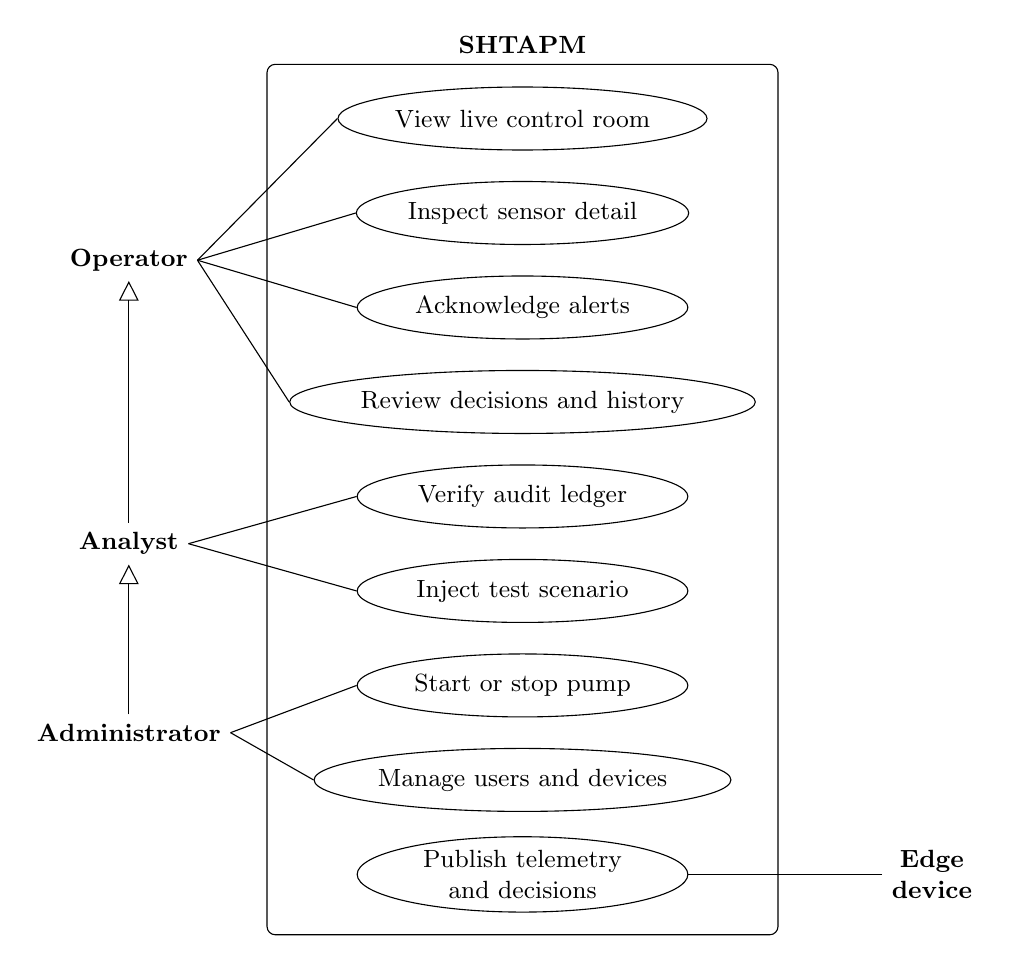
\begin{tikzpicture}[
  uc/.style={draw, ellipse, align=center, font=\small, minimum width=4.2cm, minimum height=0.8cm, inner sep=1pt},
  actor/.style={align=center, font=\small\bfseries}]
  \node[uc] (u1) at (0, 4.8) {View live control room};
  \node[uc] (u2) at (0, 3.6) {Inspect sensor detail};
  \node[uc] (u3) at (0, 2.4) {Acknowledge alerts};
  \node[uc] (u4) at (0, 1.2) {Review decisions and history};
  \node[uc] (u5) at (0, 0.0) {Verify audit ledger};
  \node[uc] (u6) at (0,-1.2) {Inject test scenario};
  \node[uc] (u7) at (0,-2.4) {Start or stop pump};
  \node[uc] (u8) at (0,-3.6) {Manage users and devices};
  \node[uc] (u9) at (0,-4.8) {Publish telemetry\\and decisions};
  \node[draw, rounded corners=3pt, fit=(u1)(u2)(u3)(u4)(u5)(u6)(u7)(u8)(u9), inner sep=8pt] (sys) {};
  \node[font=\small\bfseries, anchor=south] at (sys.north) {SHTAPM};
  \node[actor] (op) at (-5.0, 3.0) {Operator};
  \node[actor] (an) at (-5.0,-0.6) {Analyst};
  \node[actor] (ad) at (-5.0,-3.0) {Administrator};
  \node[actor] (ed) at ( 5.2,-4.8) {Edge\\device};
  \foreach \uc in {u1,u2,u3,u4} \draw (op.east) -- (\uc.west);
  \foreach \uc in {u5,u6} \draw (an.east) -- (\uc.west);
  \foreach \uc in {u7,u8} \draw (ad.east) -- (\uc.west);
  \draw[-{Triangle[open, length=2.5mm, width=2.5mm]}] (an.north) -- (op.south);
  \draw[-{Triangle[open, length=2.5mm, width=2.5mm]}] (ad.north) -- (an.south);
  \draw (ed.west) -- (u9.east);
\end{tikzpicture}
\caption{Use case diagram (open triangle: role inheritance)}
\label{fig:usecase}
\end{figure}

\subsection{Class Diagram}

\begin{sloppypar}
Figure~\ref{fig:class} shows the principal classes of the edge decision pipeline. \emph{LiveP2Monitor} owns the rolling window and runs one decision cycle per window through \emph{P2Pipeline}, which composes the \emph{Preprocessor}, the \emph{IsolationForestDetector}, the \emph{TrustEngine} and the \emph{AttributionEngine}. Isolation is tracked across cycles by the \emph{IsolationFallbackTracker}; substitution is performed by the \emph{SelfHealRuntime} using a trained \emph{LSTMTwinReconstructor}; and the \emph{SafetySupervisor} is the only component permitted to switch the relay.
\end{sloppypar}

\begin{figure}[htbp]
\centering
\begin{tikzpicture}[
  cls/.style={draw, rectangle split, rectangle split parts=2, align=left, font=\scriptsize, inner sep=3pt, text width=3.7cm, fill=white},
  node distance=0.8cm and 0.6cm]
  \node[cls] (mon) {\textbf{LiveP2Monitor}\nodepart{two}window: rolling deque\\on\_frame(frame)\\fit(baseline)};
  \node[cls, right=of mon] (pipe) {\textbf{P2Pipeline}\nodepart{two}process(frames)\\$\rightarrow$ WindowOutcome};
  \node[cls, right=of pipe] (pre) {\textbf{Preprocessor}\nodepart{two}window size 30\\process(frames)};
  \node[cls, below=of mon] (attr) {\textbf{AttributionEngine}\nodepart{two}rule: OperatingStateRule\\attribute(flags)};
  \node[cls, below=of pipe] (trust) {\textbf{TrustEngine}\nodepart{two}BetaState per channel\\update(c, k, h)};
  \node[cls, below=of pre] (det) {\textbf{IsolationForestDetector}\nodepart{two}flag threshold\\fit(), score(), flag()};
  \node[cls, below=of attr] (iso) {\textbf{IsolationFallbackTracker}\nodepart{two}tracked channels\\update(outcome)};
  \node[cls, below=of trust] (heal) {\textbf{SelfHealRuntime}\nodepart{two}SelfHealOrchestrator\\substitute(), end\_episode()};
  \node[cls, below=of det] (twin) {\textbf{LSTMTwinReconstructor}\nodepart{two}reconstruct(window, channel)};
  \node[cls, below=of heal] (safe) {\textbf{SafetySupervisor}\nodepart{two}command(), safe\_stop()\\Watchdog, DryRunDetector};

  \draw[-{Diamond[open, length=2.5mm]}] (pipe) -- (mon);
  \draw[-{Diamond[open, length=2.5mm]}] (pre) -- (pipe);
  \draw[-{Diamond[open, length=2.5mm]}] (det.north west) -- (pipe.south east);
  \draw[-{Diamond[open, length=2.5mm]}] (trust) -- (pipe);
  \draw[-{Diamond[open, length=2.5mm]}] (attr.north east) -- (pipe.south west);
  \draw[flow] (attr) -- (iso);
  \draw[flow] (iso) -- (heal);
  \draw[-{Diamond[open, length=2.5mm]}] (twin) -- (heal);
  \draw[flow] (heal) -- node[side]{escalate} (safe);
\end{tikzpicture}
\caption{Class diagram of the edge decision pipeline (open diamond: composition by reference; arrow: data dependency)}
\label{fig:class}
\end{figure}

\subsection{Sequence Diagram}

Figure~\ref{fig:sequence} traces the handling of a spoofing attack in which the motor-current reading is forced to zero while the motor is running.

\begin{figure}[htbp]
\centering
\begin{tikzpicture}[font=\scriptsize]
  \foreach \x/\n/\ttl in {0/a/Attacker, 2.4/s/Sampler, 4.8/p/Edge pipeline, 7.2/h/Self-healing, 9.6/b/Backend, 12.0/d/Dashboard}{
    \node[draw, fill=white, minimum width=2.0cm, minimum height=0.6cm, font=\small] (\n) at (\x,0) {\ttl};
    \draw[dashed, gray] (\x,-0.3) -- (\x,-11.4);
  }
  \newcommand{\msg}[4]{\draw[flow] (#1,#3) -- node[above, align=center, fill=white, inner sep=1.5pt]{#4} (#2,#3);}
  \msg{0}{2.4}{-1.0}{current set to 0 A}
  \msg{2.4}{4.8}{-1.8}{frame (1 Hz)}
  \draw[flow] (4.8,-2.5) -- ++(0.5,0) |- (4.8,-3.0);
  \node[align=left, anchor=west, fill=white, inner sep=1pt] at (5.4,-2.75) {physics check: current IDLE,\\vibration RUNNING};
  \msg{4.8}{9.6}{-3.8}{decision: attack, trust falls}
  \msg{9.6}{12.0}{-4.6}{ATTACK}
  \msg{4.8}{7.2}{-5.6}{trust $<$ 0.4: isolate}
  \msg{7.2}{9.6}{-6.4}{twin value}
  \draw[flow] (9.6,-7.1) -- ++(0.5,0) |- (9.6,-7.6);
  \node[align=left, anchor=west, fill=white, inner sep=1pt] at (10.2,-7.35) {ledger block,\\alert raised};
  \msg{9.6}{12.0}{-8.4}{VIRTUAL value}
  \msg{0}{2.4}{-9.4}{attack ends}
  \msg{4.8}{9.6}{-10.2}{trust $\geq$ 0.7: release}
  \msg{9.6}{12.0}{-11.0}{NORMAL}
\end{tikzpicture}
\caption{Sequence diagram: detecting and healing a spoofed current sensor}
\label{fig:sequence}
\end{figure}

\subsection{Activity Diagram}

Figure~\ref{fig:activity} shows the decision cycle that the edge executes for every completed window.

\begin{figure}[htbp]
\centering
\begin{tikzpicture}[
  act/.style={draw, rounded corners=6pt, align=center, font=\small, minimum width=5.6cm, minimum height=0.75cm, fill=white},
  dec/.style={draw, diamond, aspect=2.4, align=center, font=\scriptsize, inner sep=1pt, fill=white},
  node distance=0.4cm]
  \node[circle, fill=black, minimum size=0.3cm, inner sep=0pt] (start) {};
  \node[act, below=of start] (a1) {Receive frame and append to window};
  \node[act, below=of a1] (a2) {Normalise window; score with Isolation Forest};
  \node[act, below=of a2] (a3) {Compute $c$, $k$, $h$; update Beta trust per channel};
  \node[act, below=of a3] (a4) {Physics check: current state vs.\ vibration state};
  \node[dec, below=of a4] (d1) {anomaly\\flagged?};
  \node[act, below=of d1] (a5) {Attribute \textbf{attack} if physics is violated,\\otherwise \textbf{fault}};
  \node[dec, below=of a5] (d2) {trust\\$<$ 0.4?};
  \node[act, below=of d2] (a6) {Isolate channel; substitute twin value};
  \node[dec, below=of a6] (d3) {isolated\\$>$ 60 s?};
  \node[act, below=of d3] (a7) {Latched Safe Pump-Stop};
  \node[act, minimum width=2.8cm, right=1.6cm of a6] (pub) {Publish decision\\and telemetry};
  \node[circle, draw, minimum size=0.36cm, inner sep=0pt, right=0.5cm of pub] (end) {};
  \node[circle, fill=black, minimum size=0.2cm, inner sep=0pt] at (end) {};

  \draw[flow] (start) -- (a1);
  \draw[flow] (a1) -- (a2);
  \draw[flow] (a2) -- (a3);
  \draw[flow] (a3) -- (a4);
  \draw[flow] (a4) -- (d1);
  \draw[flow] (d1) -- node[side]{yes} (a5);
  \draw[flow] (a5) -- (d2);
  \draw[flow] (d2) -- node[side]{yes} (a6);
  \draw[flow] (a6) -- (d3);
  \draw[flow] (d3) -- node[side]{yes} (a7);
  \draw[flow] (d1.west) -- node[font=\scriptsize, above]{no} ($(d1.west -| a5.west)+(-0.5,0)$) |- (d2.west);
  \draw[flow] (d2.east) -| node[font=\scriptsize, pos=0.15, above]{no} (pub.north);
  \draw[flow] (d3.east) -| node[font=\scriptsize, pos=0.15, above]{no} ([xshift=-0.6cm]pub.south);
  \draw[flow] (a7.east) -| ([xshift=0.6cm]pub.south);
  \draw[flow] (pub) -- (end);
\end{tikzpicture}
\caption{Activity diagram of the per-window decision cycle}
\label{fig:activity}
\end{figure}

\subsection{State Diagram}

Every sensor channel moves through the states of Figure~\ref{fig:statechart}, driven by its trust score $T$. A channel starts \textsc{suspicious}, because the neutral Beta prior gives $T = 0.5$, and becomes \textsc{trusted} within two windows of clean evidence. It enters \textsc{isolated} when $T$ falls below 0.4, from either band, and only returns to \textsc{trusted} when $T$ reaches 0.7 again; inside the band between 0.4 and 0.7 an isolated channel stays isolated, which prevents a channel from flickering in and out of isolation. While isolated, its value is served by the digital twin, and if isolation lasts 60~s the safety supervisor stops the pump.

\begin{figure}[htbp]
\centering
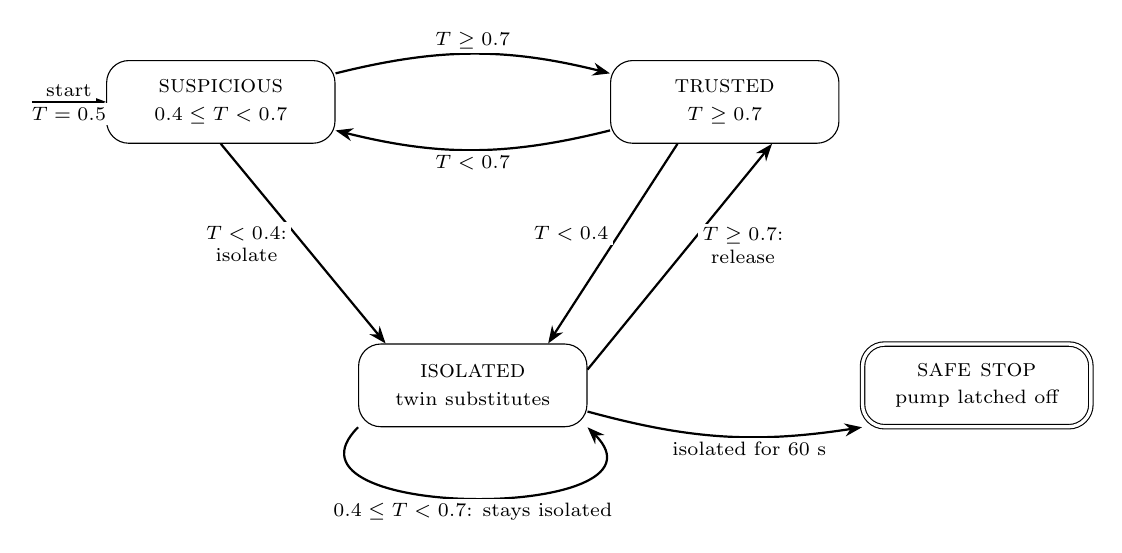
\begin{tikzpicture}[
  st/.style={draw, rounded corners=8pt, minimum width=2.9cm, minimum height=1.05cm, align=center, font=\small, fill=white},
  tr/.style={-{Stealth[length=2.2mm]}, thick},
  tl/.style={font=\scriptsize, align=center, fill=white, inner sep=1.5pt}]
  \node[st] (sus) at (0,0) {\textsc{suspicious}\\[-1pt]{\scriptsize $0.4 \leq T < 0.7$}};
  \node[st] (tru) at (6.4,0) {\textsc{trusted}\\[-1pt]{\scriptsize $T \geq 0.7$}};
  \node[st] (iso) at (3.2,-3.6) {\textsc{isolated}\\[-1pt]{\scriptsize twin substitutes}};
  \node[st, double, double distance=1.2pt] (stop) at (9.6,-3.6) {\textsc{safe stop}\\[-1pt]{\scriptsize pump latched off}};
  \draw[tr] (-2.4,0) -- node[tl, above]{start} node[tl, below]{$T = 0.5$} (sus);
  \draw[tr] (sus) to[bend left=14] node[tl, above]{$T \geq 0.7$} (tru);
  \draw[tr] (tru) to[bend left=14] node[tl, below]{$T < 0.7$} (sus);
  % isolate: from either band down into ISOLATED
  \draw[tr] (sus.south) -- node[tl, left, xshift=-4pt]{$T < 0.4$:\\isolate} ($(iso.north west)+(0.35,0)$);
  \draw[tr] ($(tru.south)+(-0.6,0)$) -- node[tl, pos=0.45, left, xshift=-2pt]{$T < 0.4$} ($(iso.north east)+(-0.5,0)$);
  % release: ISOLATED back to TRUSTED
  \draw[tr] ($(iso.east)+(0,0.2)$) -- node[tl, pos=0.55, right, xshift=3pt]{$T \geq 0.7$:\\release} ($(tru.south)+(0.6,0)$);
  % stays isolated in the Suspicious band
  \draw[tr] (iso.south west) .. controls +(-1.2,-1.2) and +(1.2,-1.2) .. node[tl, below]{$0.4 \leq T < 0.7$: stays isolated} (iso.south east);
  % budget exhausted
  \draw[tr] ($(iso.south east)+(0,0.2)$) to[bend right=12] node[tl, below, pos=0.6]{isolated for 60~s} (stop.south west);
\end{tikzpicture}
\caption{State diagram of a sensor channel}
\label{fig:statechart}
\end{figure}

\subsection{Deployment Diagram}

Figure~\ref{fig:deployment} shows how the software is distributed over the hardware. The Raspberry Pi hosts everything that must keep working without a network: the edge service with the full decision pipeline, the persisted baseline and twin bundle, and the MQTT broker. The workstation hosts the backend with its database and the development server that delivers the dashboard, and the operator's browser runs the dashboard itself.

\begin{figure}[htbp]
\centering
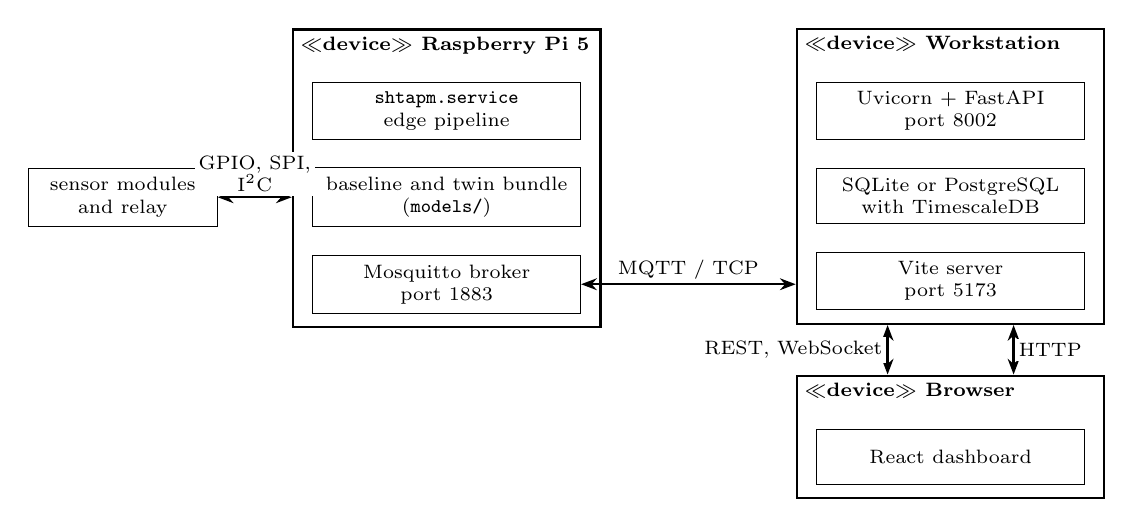
\begin{tikzpicture}[
  node distance=0.35cm,
  comp/.style={draw, align=center, font=\scriptsize, minimum width=3.4cm, minimum height=0.7cm, fill=white},
  dev/.style={draw, thick, inner sep=7pt},
  devlabel/.style={font=\scriptsize\bfseries, anchor=north west, inner sep=3pt},
  link/.style={{Stealth[length=2mm]}-{Stealth[length=2mm]}, thick},
  ll/.style={font=\scriptsize, align=center, fill=white, inner sep=1.5pt}]
  % Raspberry Pi
  \node[comp] (svc) at (0,0) {\texttt{shtapm.service}\\edge pipeline};
  \node[comp, below=of svc] (mod) {baseline and twin bundle\\(\texttt{models/})};
  \node[comp, below=of mod] (mos) {Mosquitto broker\\port 1883};
  \node[dev, fit=(svc)(mos), yshift=0.25cm, inner ysep=12pt] (pi) {};
  \node[devlabel] at (pi.north west) {$\ll$device$\gg$ Raspberry Pi 5};
  % Sensors
  \node[comp, left=1.2cm of mod, minimum width=2.4cm] (sens) {sensor modules\\and relay};
  \draw[link] (sens) -- node[ll, above]{GPIO, SPI,\\I\textsuperscript{2}C} (pi.west |- sens);
  % Workstation
  \node[comp] (api) at (6.4,0) {Uvicorn + FastAPI\\port 8002};
  \node[comp, below=of api] (db) {SQLite or PostgreSQL\\with TimescaleDB};
  \node[comp, below=of db] (vite) {Vite server\\port 5173};
  \node[dev, fit=(api)(vite), yshift=0.25cm, inner ysep=12pt] (ws) {};
  \node[devlabel] at (ws.north west) {$\ll$device$\gg$ Workstation};
  % Browser
  \node[comp, below=1.5cm of vite] (react) {React dashboard};
  \node[dev, fit=(react), yshift=0.25cm, inner ysep=12pt] (br) {};
  \node[devlabel] at (br.north west) {$\ll$device$\gg$ Browser};
  \draw[link] (mos.east) -- node[ll, above]{MQTT / TCP} (mos.east -| ws.west);
  \draw[link] ($(br.north)+(-0.8,0)$) -- node[ll, left]{REST, WebSocket} ($(ws.south)+(-0.8,0)$);
  \draw[link] ($(br.north)+(0.8,0)$) -- node[ll, right]{HTTP} ($(ws.south)+(0.8,0)$);
\end{tikzpicture}
\caption{Deployment diagram}
\label{fig:deployment}
\end{figure}

\section{Module Description}

Table~\ref{tab:modules} lists the modules of the system and the responsibility of each. Their implementation is described in Chapter~\ref{ch:implementation}.

\begin{table}[htbp]
\centering
\caption{System modules and their responsibilities}
\label{tab:modules}
\small
\begin{tabularx}{\textwidth}{@{}P{3.4cm} X@{}}
\toprule
\textbf{Module} & \textbf{Responsibility} \\
\midrule
Sensor drivers & One driver per physical device (DHT22, ADXL335 with MCP3008, BMP280, INA219, MQ-135) behind a common interface that returns a value, a unit and a health flag. \\
Acquisition & 1~Hz sampler that assembles contract-valid frames, holds the last good value of a failing channel and declares a sensor dead after 5~s of continuous failure. \\
Preprocessing & Rolling window of 30 samples per channel with per-window normalisation. \\
Anomaly detection & Isolation Forest fitted on recorded clean windows; the severity of a window is the empirical rank of its score within the clean distribution. \\
Trust engine & Per-channel Beta-reputation state, updated every window from consistency ($c$), physical-correlation ($k$) and historical-reliability ($h$) evidence. \\
Attribution & Operating-state rule that classifies current and vibration as idle or running using bands learned from the baseline; a contradiction is an attack on the channel that changed state alone. \\
Isolation and self-healing & Tracks channels whose trust falls below 0.4, substitutes an LSTM digital-twin reconstruction and releases the channel when trust returns to 0.7. \\
Safety supervisor & Sole owner of the relay: operator commands, Safe Pump-Stop after 60~s of substitution, a 10~s watchdog and dry-run detection, all latching. \\
Messaging & MQTT topics for telemetry, decision diagnostics, commands and actuation status. \\
Backend services & Persistence, alert generation, device-condition rollup, sensor-health tracking, live physics state and the SHA-256 audit ledger, exposed through authenticated REST and WebSocket endpoints. \\
Dashboard & Control room, sensor detail, devices, device, decisions, history, alerts, ledger, users, system and settings pages. \\
\bottomrule
\end{tabularx}
\end{table}

\section{Database Design}

The backend stores its data in ten relational tables (Figure~\ref{fig:er}). The data model is written once with SQLAlchemy and runs unchanged on SQLite for development and tests and on PostgreSQL in deployment, where the two high-volume time-series tables, \texttt{sensor\_readings} and \texttt{decisions}, become TimescaleDB hypertables partitioned by time.

\begin{figure}[htbp]
\centering
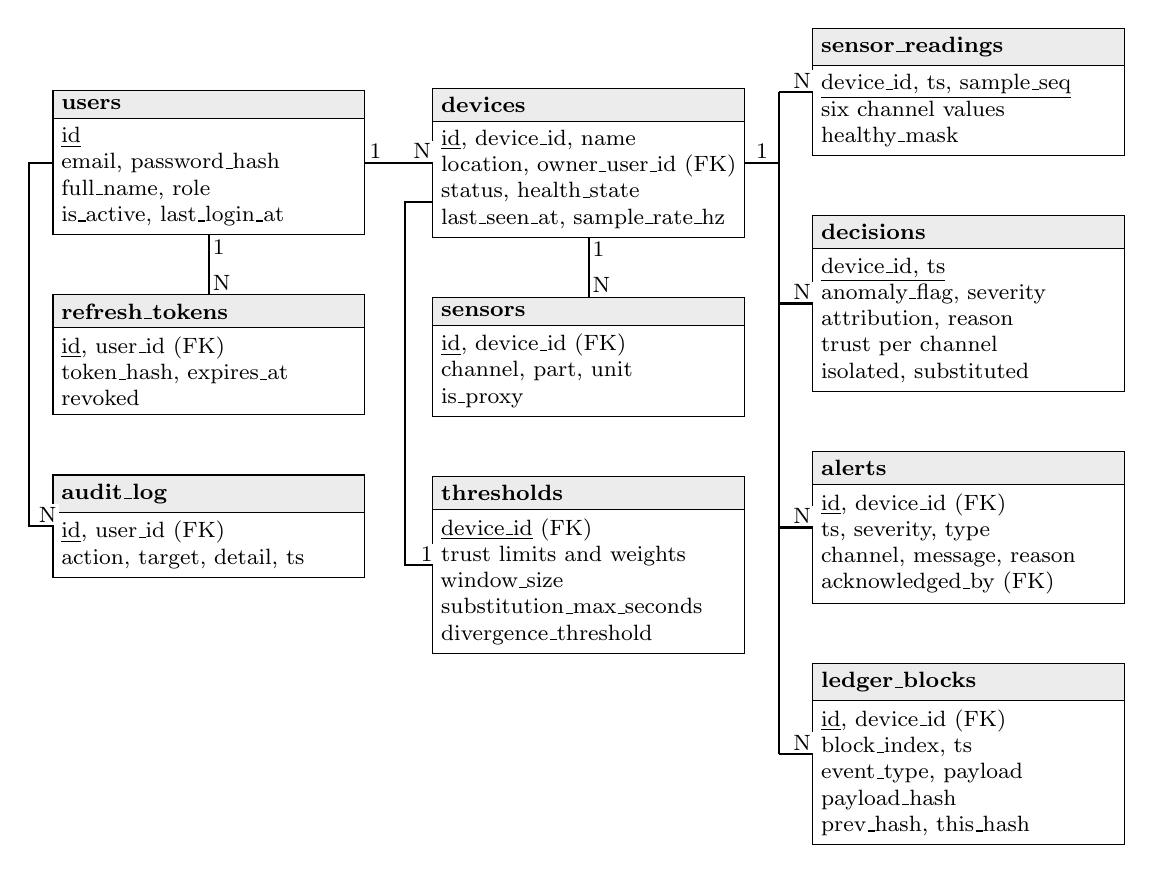
\begin{tikzpicture}[
  ent/.style={draw, rectangle split, rectangle split parts=2, rectangle split part fill={gray!15,white}, align=left, font=\footnotesize, inner sep=3pt, text width=3.75cm},
  rel/.style={thick},
  card/.style={font=\footnotesize, inner sep=1pt, fill=white},
  node distance=0.75cm and 0.85cm]
  \node[ent] (users) {\textbf{users}\nodepart{two}\underline{id}\\email, password\_hash\\full\_name, role\\is\_active, last\_login\_at};
  \node[ent, below=of users] (rt) {\textbf{refresh\_tokens}\nodepart{two}\underline{id}, user\_id (FK)\\token\_hash, expires\_at\\revoked};
  \node[ent, below=of rt] (audit) {\textbf{audit\_log}\nodepart{two}\underline{id}, user\_id (FK)\\action, target, detail, ts};
  \node[ent, right=of users] (dev) {\textbf{devices}\nodepart{two}\underline{id}, device\_id, name\\location, owner\_user\_id (FK)\\status, health\_state\\last\_seen\_at, sample\_rate\_hz};
  \node[ent, below=of dev] (sen) {\textbf{sensors}\nodepart{two}\underline{id}, device\_id (FK)\\channel, part, unit\\is\_proxy};
  \node[ent, below=of sen] (thr) {\textbf{thresholds}\nodepart{two}\underline{device\_id} (FK)\\trust limits and weights\\window\_size\\substitution\_max\_seconds\\divergence\_threshold};
  \node[ent, right=of dev, yshift=0.9cm] (read) {\textbf{sensor\_readings}\nodepart{two}\underline{device\_id, ts, sample\_seq}\\six channel values\\healthy\_mask};
  \node[ent, below=of read] (dec) {\textbf{decisions}\nodepart{two}\underline{device\_id, ts}\\anomaly\_flag, severity\\attribution, reason\\trust per channel\\isolated, substituted};
  \node[ent, below=of dec] (al) {\textbf{alerts}\nodepart{two}\underline{id}, device\_id (FK)\\ts, severity, type\\channel, message, reason\\acknowledged\_by (FK)};
  \node[ent, below=of al] (led) {\textbf{ledger\_blocks}\nodepart{two}\underline{id}, device\_id (FK)\\block\_index, ts\\event\_type, payload\\payload\_hash\\prev\_hash, this\_hash};

  \draw[rel] (users) -- node[card, above, pos=0.15]{1} node[card, above, pos=0.85]{N} (dev);
  \draw[rel] (users) -- node[card, right, pos=0.2]{1} node[card, right, pos=0.8]{N} (rt);
  \draw[rel] (users.west) -- ++(-0.3,0) |- node[card, above, pos=0.9]{N} (audit.west);
  \draw[rel] (dev) -- node[card, right, pos=0.2]{1} node[card, right, pos=0.8]{N} (sen);
  \draw[rel] (dev.west) ++(0,-0.5) -- ++(-0.35,0) |- node[card, above, pos=0.9]{1} (thr.west);
  \coordinate (bus) at ($(dev.east)!0.5!(dev.east -| read.west)$);
  \draw[rel] (dev.east) -- node[card, above, pos=0.5]{1} (bus);
  \draw[rel] (bus |- read.west) -- (bus |- led.west);
  \foreach \tb in {read, dec, al, led}
    \draw[rel] (bus |- \tb.west) -- node[card, above, pos=0.7]{N} (\tb.west);
\end{tikzpicture}
\caption{Entity--relationship diagram of the backend database (underlined: primary key; FK: foreign key)}
\label{fig:er}
\end{figure}

\begin{table}[htbp]
\centering
\caption{Database tables}
\label{tab:tables}
\small
\begin{tabularx}{\textwidth}{@{}P{3.6cm} X@{}}
\toprule
\textbf{Table} & \textbf{Purpose} \\
\midrule
\texttt{users} & Accounts with a bcrypt password hash and one of three roles \\
\texttt{refresh\_tokens} & Hashed refresh tokens, rotated on use and revoked on logout \\
\texttt{audit\_log} & Every privileged action and every denied request, with the acting user \\
\texttt{devices} & Monitored pumps with their owner, status, condition and sampling rate \\
\texttt{sensors} & The channels of each device, with part, unit and whether the channel is a stand-in \\
\texttt{thresholds} & Per-device trust limits, evidence weights, window size and substitution budget \\
\texttt{sensor\_readings} & One row per telemetry frame with all six values and a per-channel health mask \\
\texttt{decisions} & One row per decision window: anomaly, attribution, reason, trust, isolation and substitution \\
\texttt{alerts} & Operator alerts with severity, type and acknowledgement \\
\texttt{ledger\_blocks} & The hash chain of safety-relevant events \\
\bottomrule
\end{tabularx}
\end{table}

\section{Communication Design}

All edge--backend communication uses MQTT topics under a per-device prefix (Table~\ref{tab:topics}). Quality of service is chosen per stream: telemetry and decisions use QoS~0, because a newer frame supersedes a lost one within a second, while status, actuation and commands use QoS~1, because a lost relay command or status change must be redelivered. Device status and actuation status are \emph{retained}, so a backend that restarts immediately learns whether the edge is online and what state the relay is in. The edge registers a last-will message, so the broker itself announces \texttt{offline} if the edge disappears without warning.

\begin{table}[htbp]
\centering
\caption{MQTT topic design (prefix \texttt{shtapm/\{device\_id\}/})}
\label{tab:topics}
\small
\begin{tabularx}{\textwidth}{@{}P{3.9cm} P{2.7cm} c c X@{}}
\toprule
\textbf{Topic} & \textbf{Direction} & \textbf{QoS} & \textbf{Retained} & \textbf{Content} \\
\midrule
\texttt{telemetry} & Edge $\rightarrow$ backend & 0 & No & One frame per second \\
\texttt{decision\_\allowbreak diagnostic} & Edge $\rightarrow$ backend & 0 & No & One decision per window \\
\texttt{status} & Edge $\rightarrow$ backend & 1 & Yes & \texttt{online} or \texttt{offline} (last will) \\
\texttt{actuation} & Edge $\rightarrow$ backend & 1 & Yes & Relay state, cause, latched flag \\
\texttt{command} & Backend $\rightarrow$ edge & 1 & No & Start or cancel a test scenario \\
\texttt{relay\_command} & Backend $\rightarrow$ edge & 1 & No & Switch the pump on or off \\
\bottomrule
\end{tabularx}
\end{table}

Between the backend and the dashboard, the authenticated WebSocket carries the live telemetry stream so that trends update with every sample, and REST endpoints serve everything else: history, decisions, alerts, ledger, live physics state and relay state, which the dashboard polls at intervals between one and five seconds. Relay commands deliberately travel on their own topic, separate from scenario commands, so a test injection can never reach the pump.

\section{User Interface Design}

The dashboard was designed for the operator of an unmanned station who glances at it occasionally and must understand the situation within seconds. Following ANSI/ISA-101~\cite{isa101}, its design rests on four principles.

\begin{enumerate}
  \item \textbf{Calm when normal.} During normal operation the display is neutral and grey, so that anything coloured is, by definition, something that needs attention.
  \item \textbf{Colour carries meaning, never decoration.} Each colour has exactly one meaning throughout the application (Table~\ref{tab:colours}).
  \item \textbf{Never by colour alone.} Every state is also written in words (\textsc{attack}, \textsc{fault}, \textsc{virtual}), so it remains readable for colour-blind users and on monochrome printouts.
  \item \textbf{Explain, then act.} Every verdict shows its reason, and every isolation shows the twin's value next to the sensor's rejected reading, so that the operator can check the system's reasoning.
\end{enumerate}

\begin{table}[htbp]
\centering
\caption{Colour semantics of the dashboard}
\label{tab:colours}
\small
\begin{tabularx}{\textwidth}{@{}P{2.4cm} P{3.4cm} X@{}}
\toprule
\textbf{Colour} & \textbf{Meaning} & \textbf{Used for} \\
\midrule
Neutral grey & Normal & Values, trends and panels in normal operation \\
Green & Healthy, trusted & Trust above 0.7, healthy device, physics agreeing \\
Amber & Fault, warning & Physically consistent anomalies, warning condition \\
Red & Attack, critical & Physics violations, malicious trust, Safe Pump-Stop \\
Violet & Virtual & Values served by the digital twin, isolated channels \\
Blue & Information & Navigation, selection and the live sensor marker \\
\bottomrule
\end{tabularx}
\end{table}

Figure~\ref{fig:navigation} shows the navigation structure. After signing in, every page is one click away in a persistent sidebar, grouped by the operator's purpose: monitoring, analysis, assets, assurance and administration. The control room is the home page, any sensor opens a detail panel over it without leaving the page, and alert pop-ups appear on every page. Administrative pages are shown only to users whose role permits them.

\begin{figure}[htbp]
\centering
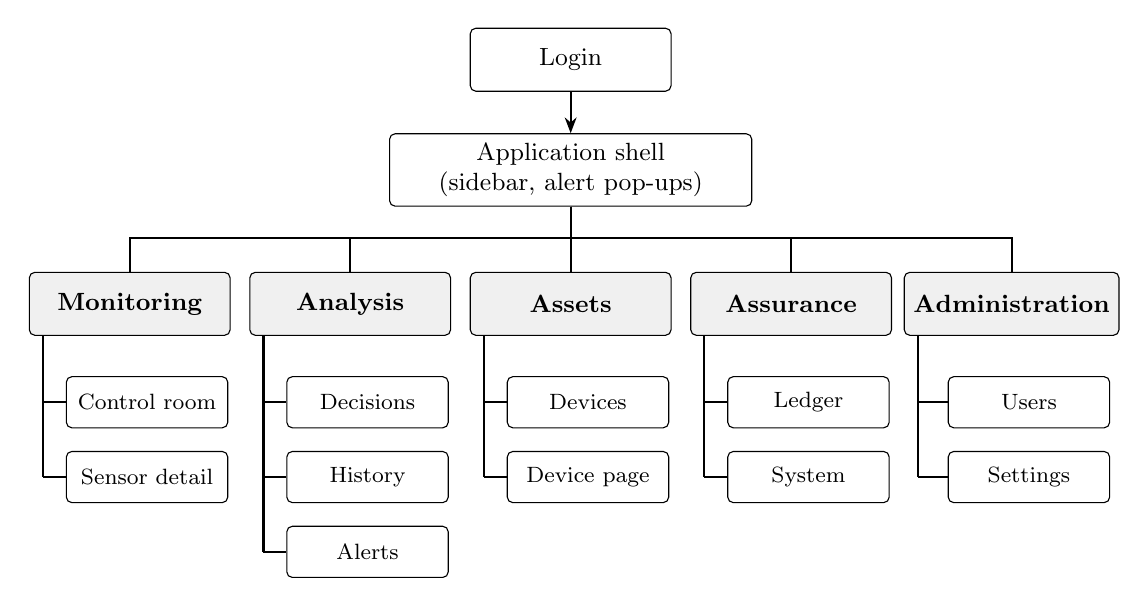
\begin{tikzpicture}[
  pg/.style={draw, rounded corners=2pt, font=\small, align=center, minimum width=2.55cm, minimum height=0.8cm, fill=white},
  grp/.style={pg, font=\small\bfseries, fill=gray!12},
  ln/.style={thick}]
  \node[pg] (login) at (5.6,0) {Login};
  \node[pg, minimum width=4.6cm] (shell) at (5.6,-1.4) {Application shell\\(sidebar, alert pop-ups)};
  \draw[ln, -{Stealth[length=2mm]}] (login) -- (shell);
  \foreach \x/\g/\name in {0/m/Monitoring, 2.8/a/Analysis, 5.6/s/Assets, 8.4/q/Assurance, 11.2/d/Administration} {
    \node[grp] (\g) at (\x,-3.1) {\name};
    \draw[ln] (shell.south) -- ++(0,-0.4) -| (\g.north);
  }
  \foreach \g/\list in {m/{Control room,Sensor detail}, a/{Decisions,History,Alerts}, s/{Devices,Device page}, q/{Ledger,System}, d/{Users,Settings}} {
    \foreach \p [count=\i] in \list {
      \node[pg, font=\footnotesize, minimum height=0.65cm, minimum width=2.05cm] (\g\i) at ($(\g)+(0.22,-0.95*\i-0.3)$) {\p};
    }
  }
  \foreach \g/\n in {m/2, a/3, s/2, q/2, d/2} {
    \draw[ln] (\g.south west) ++(0.18,0) coordinate (rail\g) -- (rail\g |- \g\n.west);
    \foreach \i in {1,...,\n}
      \draw[ln] (rail\g |- \g\i.west) -- (\g\i.west);
  }
\end{tikzpicture}
\caption{Navigation structure of the dashboard: every page is one click away in the sidebar, grouped by purpose}
\label{fig:navigation}
\end{figure}

\chapter{System Requirement Specification}
\label{ch:srs}

This chapter specifies what SHTAPM must do and what it runs on. The functional and non-functional requirements were fixed in the product requirements document at the start of the project and are referred to by their identifiers throughout the rest of this report.

\section{Functional Requirements}

Table~\ref{tab:fr} lists the functional requirements grouped by subsystem.

{\small
\setlength{\LTpre}{0pt}
\begin{longtable}{@{}P{1.6cm} P{12.2cm}@{}}
\caption{Functional requirements}
\label{tab:fr}\\
\toprule
\textbf{ID} & \textbf{Requirement} \\
\midrule
\endfirsthead
\toprule
\textbf{ID} & \textbf{Requirement} \\
\midrule
\endhead
\bottomrule
\endfoot
\multicolumn{2}{@{}l}{\textit{Acquisition}} \\
FR-Q1 & Sample all six sensor channels at a configurable rate (default 1~Hz). \\
FR-Q2 & Tag each frame with the device identifier, an ISO-8601 timestamp and a sequence number. \\
FR-Q3 & Publish frames to an MQTT broker on a per-device topic. \\
FR-Q4 & Buffer locally and resume publishing after a broker disconnection. \\
\multicolumn{2}{@{}l}{\textit{Preprocessing}} \\
FR-P1 & Apply noise filtering, min--max normalisation and missing-value handling. \\
FR-P2 & Assemble sliding windows of 30 samples per channel. \\
\multicolumn{2}{@{}l}{\textit{Anomaly detection and attribution}} \\
FR-A1 & Flag statistical anomalies per window with an Isolation Forest trained on clean baseline data. \\
FR-A2 & Use cross-sensor physics checks to classify an anomaly as a physical fault or a cyber-attack. \\
FR-A3 & Output an anomaly flag, a severity, an attribution label and a reason. \\
FR-A4 & Accept fault and attack scenarios injected by an authorised user through an authenticated control channel. \\
\multicolumn{2}{@{}l}{\textit{Trust}} \\
FR-T1 & Maintain a per-sensor trust score $T \in [0, 1]$ with a Beta-reputation model updated every window. \\
FR-T2 & Weight consistency, cross-sensor correlation and historical reliability in the trust update. \\
FR-T3 & Classify each sensor as Trusted ($T \geq 0.7$), Suspicious ($0.4 \leq T < 0.7$) or Malicious ($T < 0.4$). \\
FR-T4 & Let trust recover when a sensor returns to consistent behaviour. \\
\multicolumn{2}{@{}l}{\textit{Self-healing}} \\
FR-H1 & Remove an isolated sensor from fusion. \\
FR-H2 & Reconstruct an isolated sensor's value through an LSTM digital twin, with an uncertainty estimate. \\
FR-H3 & Bound substitution in time and escalate to a Safe Pump-Stop when the bound is exceeded. \\
FR-H4 & Heal without human action within one processing cycle of the decision. \\
\multicolumn{2}{@{}l}{\textit{Safety}} \\
FR-R1 & Drive the pump relay to stop the pump on command. \\
FR-R2 & Stop the pump autonomously on a dry-run signature. \\
FR-R3 & Default the pump to a safe state through a watchdog if the edge node fails. \\
\multicolumn{2}{@{}l}{\textit{Audit ledger}} \\
FR-L1 & Write every trust drop, anomaly, response action and heal as a hash-chained block. \\
FR-L2 & Detect any tampering with a previous block through a verifier. \\
FR-L3 & Make ledger entries queryable from the dashboard. \\
\multicolumn{2}{@{}l}{\textit{Dashboard}} \\
FR-D1 & Render live per-sensor time series that update in real time. \\
FR-D2 & Show a per-sensor trust panel and a machine-health indicator. \\
FR-D3 & Show the decision log and the ledger event stream. \\
FR-D4 & Surface active alerts with severity and reason. \\
FR-D5 & Show system health: broker connectivity, sample rate and end-to-end latency. \\
FR-D6 & Allow administrators to configure thresholds and register devices. \\
FR-D7 & Provide an authenticated scenario-injection control. \\
FR-D8 & Visibly mark any channel currently served by digital-twin substitution. \\
\end{longtable}
}

The original requirement set also included a learned remaining-useful-life prognosis model and a reinforcement-learning response policy. Their implementation status is described in Section~\ref{sec:impl-prognosis-rl} and their completion is part of the future work in Chapter~\ref{ch:conclusion}.

\section{Non-Functional Requirements}

Table~\ref{tab:nfr} lists the quality attributes the system must meet, each with a measurable target.

\begin{table}[htbp]
\centering
\caption{Non-functional requirements}
\label{tab:nfr}
\small
\begin{tabularx}{\textwidth}{@{}l l X l@{}}
\toprule
\textbf{ID} & \textbf{Category} & \textbf{Requirement} & \textbf{Target} \\
\midrule
NFR-P1 & Performance & End-to-end latency, sensor event to dashboard & $<$ 2~s \\
NFR-P2 & Performance & Sense--decide--act cycle at the edge & $<$ 2~s \\
NFR-R1 & Reliability & Continuous operation through the loss of one sensor & No crash \\
NFR-R2 & Reliability & Broker reconnection with buffered resume & 60~s retained \\
NFR-S1 & Security & Authentication and role-based access on control endpoints & Enforced \\
NFR-S2 & Security & Ledger integrity & 100\% detectable \\
NFR-SC1 & Scalability & Logical device model & $N$ devices \\
NFR-U1 & Usability & Operator assesses station status at a glance & $\leq$ 5~s \\
NFR-U2 & Usability & Responsive layout, desktop first, tablet supported & $\geq$ 768~px \\
NFR-M1 & Maintainability & Modular subsystems with defined input/output contracts & Per module \\
NFR-O1 & Observability & Structured logs and health metrics & Edge, backend \\
\bottomrule
\end{tabularx}
\end{table}

\section{Software Requirement}

Table~\ref{tab:software} lists the software stack. Versions are those pinned in the project's dependency manifests.

\begin{table}[htbp]
\centering
\caption{Software requirements}
\label{tab:software}
\small
\begin{tabularx}{\textwidth}{@{}P{2.5cm} P{4.4cm} P{2.0cm} X@{}}
\toprule
\textbf{Layer} & \textbf{Component} & \textbf{Version} & \textbf{Purpose} \\
\midrule
Edge OS & Raspberry Pi OS (64-bit) & Bookworm & Operating system of the edge node \\
Language & Python & $\geq$ 3.11 & Edge pipeline and backend \\
Edge I/O & smbus2, spidev & 0.4, 3.8 & I\textsuperscript{2}C and SPI access \\
Sensor library & adafruit-circuitpython-dht & -- & DHT22 access \\
Machine learning & scikit-learn & 1.5 & Isolation Forest \\
Deep learning & PyTorch & 2.2 & LSTM digital twin \\
Messaging & Eclipse Mosquitto & 2.0 & MQTT broker \\
MQTT client & paho-mqtt & 1.6 & Edge publisher, backend subscriber \\
Contract & Pydantic & 2 & Shared telemetry and decision schemas \\
Backend & FastAPI, Uvicorn & 0.110, 0.29 & REST and WebSocket server \\
Persistence & SQLAlchemy, Alembic & 2.0, 1.13 & ORM and schema migrations \\
Database & PostgreSQL with TimescaleDB; SQLite & 16; 3 & Deployment target; bench and tests \\
Security & python-jose, passlib (bcrypt) & 3.3, 1.7 & JSON Web Tokens, password hashing \\
Frontend & React, TypeScript & 18.2, 5.4 & Dashboard \\
Build & Vite & 5.2 & Development server and bundler \\
Testing & pytest, Vitest, Testing Library & 8, 1.6, 16 & Automated tests \\
Quality & ruff, black, ESLint, Prettier & 0.6, 24, 8.57, 3.3 & Linting, formatting \\
Tools & Git, Visual Studio Code & -- & Version control and editing \\
\bottomrule
\end{tabularx}
\end{table}

The edge needs only the acquisition and detection dependencies at run time; PyTorch is additionally installed on the edge to run the digital twin, which is trained offline on a workstation. The backend and dashboard run on any workstation with Python and Node.js; the dashboard is served to a standard web browser.

\section{Hardware Requirement}

Table~\ref{tab:hardware} lists the hardware of the prototype rig and Table~\ref{tab:pinmap} the bus and pin assignment on the Raspberry Pi.

\begin{table}[htbp]
\centering
\caption{Hardware requirements}
\label{tab:hardware}
\small
\begin{tabularx}{\textwidth}{@{}l X l@{}}
\toprule
\textbf{Component} & \textbf{Specification} & \textbf{Role} \\
\midrule
Raspberry Pi 5 & Quad-core Arm Cortex-A76, 2.4~GHz; GPIO, SPI, I\textsuperscript{2}C & Edge node \\
microSD card & Operating system, baseline captures and models & Edge storage \\
DHT22 (AM2302) & $-40$ to $80\,^{\circ}$C, $\pm 0.5\,^{\circ}$C; 0--100\% RH, $\pm 2$--5\% & Temperature, humidity \\
ADXL335 & Three-axis analogue accelerometer, $\pm 3$~g & Vibration \\
MCP3008 & 8-channel, 10-bit SPI analogue-to-digital converter & ADC for ADXL335, MQ-135 \\
BMP280 & 300--1100~hPa, $\pm 1$~hPa, I\textsuperscript{2}C & Barometric pressure \\
INA219 & High-side current monitor, 0.1~$\Omega$ shunt, I\textsuperscript{2}C & Motor current \\
MQ-135 & Air-quality (gas) sensor, analogue output, 5~V heater & Gas \\
Relay module & Single channel, 5~V coil, normally-open contact & Pump switching \\
DC motor & 130-size brushed DC motor, 5~V supply & Pump stand-in \\
Workstation & Laptop with Python and Node.js; same network as the edge & Backend, dashboard \\
Miscellaneous & Breadboard, jumper wires, 10~k$\Omega$ and 13~k$\Omega$ divider resistors & Wiring \\
\bottomrule
\end{tabularx}
\end{table}

\begin{table}[htbp]
\centering
\caption{Bus and pin assignment on the Raspberry Pi}
\label{tab:pinmap}
\small
\begin{tabularx}{\textwidth}{@{}l l X@{}}
\toprule
\textbf{Device} & \textbf{Interface} & \textbf{Connection} \\
\midrule
DHT22 & Single-wire GPIO & GPIO17 \\
MCP3008 & SPI0, CE0 & 1.35~MHz clock; channels 0--2 carry ADXL335 X, Y, Z \\
MQ-135 & MCP3008 channel 3 & Analogue output through a 10~k$\Omega$/13~k$\Omega$ divider so the input never exceeds 3.3~V \\
BMP280 & I\textsuperscript{2}C bus 1 & Address 0x76 \\
INA219 & I\textsuperscript{2}C bus 1 & Address 0x40; shunt in series with the motor supply \\
Relay & GPIO & GPIO27 (physical pin 13); motor supply through the normally-open contact \\
\bottomrule
\end{tabularx}
\end{table}

\subsection{Prototype Configuration}

Figure~\ref{fig:rig} shows the assembled bench rig. Every channel is implemented end to end in software, from driver to dashboard. Each channel's driver is selected by configuration, so the same edge build runs on the physical sensor or on an emulated source with an identical data path. Table~\ref{tab:protoconfig} records the configuration of the prototype used for the experiments in Chapter~\ref{ch:results}.

\begin{table}[htbp]
\centering
\caption{Configuration of the prototype used for the experiments}
\label{tab:protoconfig}
\small
\begin{tabularx}{\textwidth}{@{}l l X@{}}
\toprule
\textbf{Channel} & \textbf{Device} & \textbf{Prototype configuration} \\
\midrule
Temperature & DHT22 & Physical sensor \\
Humidity & DHT22 & Physical sensor \\
Vibration & ADXL335 + MCP3008 & Physical sensor, mounted on the motor body \\
Pressure & BMP280 & Physical sensor \\
Current & INA219 & Physical sensor, in series with the motor supply \\
Gas & MQ-135 & Driver and signal conditioning implemented; experiments used the emulated source \\
Pump relay & Relay module & Driver and safety logic implemented; experiments used the in-memory relay \\
\bottomrule
\end{tabularx}
\end{table}

\screenshot{bench-rig.jpg}{0.55}{The bench prototype rig: Raspberry Pi~5 edge node, sensor modules on the breadboard and the DC motor}{fig:rig}

\chapter{Implementation}
\label{ch:implementation}

This chapter describes how the design of Chapter~\ref{ch:design} was realised: the implementation platform, the models and algorithms of every stage of the pipeline, and the functional behaviour of the complete system.

\section{Selection of Platform/Programming Language}

\subsection{Choice of Platform and Languages}

\begin{itemize}
  \item \textbf{Raspberry Pi 5 as the edge computer.} A single-board Linux computer runs the complete detection, trust, self-healing and safety pipeline next to the pump, including Isolation Forest scoring and LSTM inference, while exposing the GPIO, SPI and I\textsuperscript{2}C buses that the sensors need. A microcontroller could sample the sensors but could not host the learning models; a remote server could host the models but would put the network inside the safety loop.
  \item \textbf{Python for the edge and the backend.} Python has mature libraries for every part of the system (smbus2 and spidev for the buses, scikit-learn and PyTorch for the models, FastAPI and SQLAlchemy for the service), and one language on both sides allows the edge and the backend to share a single, validated definition of every message.
  \item \textbf{MQTT for messaging.} MQTT is a lightweight publish--subscribe protocol designed for telemetry from constrained devices. Its retained messages and last-will mechanism report device status, and a local broker keeps the system independent of external networks.
  \item \textbf{TypeScript and React for the dashboard.} Static typing catches contract mismatches at build time, and React's component model suits a live display that updates many independent panels every second.
\end{itemize}

\subsection{Repository Organisation}

The system is developed as a single Git repository (a monorepo) with one directory per deployable unit. The edge and the backend share one Python package for the wire contract, so a change to a message format is checked against both sides by the same tests.

\begin{lstlisting}[float=htbp, caption={Top-level structure of the repository}, label={lst:tree}]
SHTAPM/
  edge/        acquisition, drivers, anomaly, trust, pipeline,
               models, actuation, injection, eval, scripts
  backend/     app/api, app/services, app/mqtt, app/ws,
               app/models, app/schemas, alembic, tests
  frontend/    src/app, src/pages, src/features, src/styles
  simulator/   hardware-free telemetry source for development
  infra/       broker configuration, systemd unit
  scripts/     pre-flight self-check, utilities
  docs/        requirements, design and implementation plan
\end{lstlisting}

\subsection{Deployment}

The edge software runs on the Raspberry Pi as the \texttt{systemd} service \texttt{shtapm}, which starts at boot, restarts on failure and releases the relay pin when it stops. The Mosquitto broker runs on the Pi as well, so the edge never depends on another machine to publish. The backend (Uvicorn serving FastAPI) and the dashboard (served by Vite) run on a workstation on the same network. All configuration is read from environment variables: sensor driver selection, sampling rate, window size, broker address, relay pin and polarity, and the location of the persisted baseline and digital-twin bundle. Secrets such as the token-signing key and database password are never stored in the repository.

\subsection{Data Contract}

Every component exchanges the same frozen telemetry frame, defined once as a Pydantic model. Listing~\ref{lst:frame} shows a frame recorded on the rig.

\begin{lstlisting}[float=htbp, caption={A telemetry frame recorded on the bench rig}, label={lst:frame}]
{"device_id": "pump-01",
 "ts": "2026-10-28T07:47:32.955Z",
 "sensors": {"temperature": 27.1, "vibration": 0.0138,
             "pressure": 913.71, "humidity": 49.1,
             "gas": 148.34, "current": 0.0},
 "sample_seq": 55}
\end{lstlisting}

A decision message carries, for each window, the anomaly flag, severity, attribution (\texttt{none}, \texttt{fault} or \texttt{attack}), a reason, the trust score of every channel, the set of isolated channels and the value substituted for each. A ledger message carries an event type and its payload.

\section{Model Implementation \& Algorithm}

\subsection{Acquisition and Sensor Health}

The sampler reads every driver once per second and assembles a frame. A driver that fails to answer does not stop the frame: its last good value is held, and the channel is reported dead only after 5~s of continuous failure, so that the brief dropouts of the DHT22 when the motor starts are absorbed. Two driver-level safeguards were added after faults observed on the bench: a DHT22 reader that has failed continuously for 10~s re-opens the device, and an ADXL335 reading at either rail of the 10-bit converter (0 or 1023 counts) is treated as a failed read, because it indicates a loose connection rather than a real acceleration.

\subsection{Sensor Drivers and Signal Conversion}

Each driver converts the raw output of its device into engineering units.

\paragraph{Vibration (ADXL335 through MCP3008).} The MCP3008 returns a 10-bit count $n \in [0, 1023]$ per axis with a 3.3~V reference, and the ADXL335 has a nominal sensitivity of $S = 0.330$~V/$g$ at a 3.3~V supply, so one count corresponds to
\begin{equation}
\Delta a = \frac{V_{\mathrm{ref}}}{1024\, S} = \frac{3.3}{1024 \times 0.330} \approx 9.77 \times 10^{-3}~g.
\end{equation}
The first successful read establishes an at-rest baseline $(n_x^0, n_y^0, n_z^0)$, which absorbs each axis's zero-$g$ offset and the static gravity component, and vibration is reported as the magnitude of the deviation from it:
\begin{equation}
v = \Delta a \sqrt{(n_x - n_x^0)^2 + (n_y - n_y^0)^2 + (n_z - n_z^0)^2}.
\end{equation}
This makes vibration a relative quantity that is zero for a still motor in any mounting orientation.

\paragraph{Current (INA219).} The INA219 measures the voltage across a 0.1~$\Omega$ shunt in series with the motor supply. For a maximum expected current of 5~A, the current resolution and the calibration register value are
\begin{equation}
I_{\mathrm{LSB}} = \frac{5}{32767} \approx 1.526 \times 10^{-4}~\mathrm{A}, \qquad
\mathrm{Cal} = \left\lfloor \frac{0.04096}{I_{\mathrm{LSB}}\, R_{\mathrm{shunt}}} \right\rfloor = 2684,
\end{equation}
and the current is the signed register value multiplied by $I_{\mathrm{LSB}}$.

\paragraph{Pressure (BMP280).} The BMP280 is triggered in forced mode for one conversion per sample, and its raw temperature and pressure words are converted with the manufacturer's integer compensation formulas and the twelve calibration coefficients read from the device at start-up.

\paragraph{Temperature and humidity (DHT22).} The DHT22 transmits a 40-bit frame over a single-wire protocol containing humidity, temperature and a checksum. Reads that fail the checksum or time out are reported as failed reads and handled by the hold-last-value logic described above.

\paragraph{Gas (MQ-135).} The analogue output of the MQ-135 can exceed the converter's 3.3~V range, so it passes through a resistor divider of 10~k$\Omega$ and 13~k$\Omega$ into MCP3008 channel~3, and the driver restores the sensor voltage with the divider ratio $(10 + 13)/13 = 1.769$. The channel is reported in volts: converting the voltage to a gas concentration in parts per million requires a clean-air calibration of the individual sensor, and no unvalidated concentration is reported.

Both converter-based channels reject readings at either rail of the converter, and the DHT22 reader is re-opened after 10~s of continuous failure, as described in the previous section.

\subsection{Baseline Recording and Calibration}

The detector, the consistency and reliability evidence, the channel flag policy and the vibration bands are all fitted on a recording of clean operation of the actual rig. The procedure used for the deployed baseline was:

\begin{enumerate}
  \item Record telemetry on the Pi for about 50 minutes while switching the motor on and off by hand at irregular intervals, so that both motor states and many transitions are represented.
  \item A few minutes into the recording, and again later, run a recording check that splits the frames by motor state using the current (idle below 0.05~A, running above 0.3~A) and reports, per five-minute block, the median idle and running vibration, frame gaps and missing values. The check fails if idle vibration exceeds 0.5~$g$ (the sensor has moved), if running vibration is not at least twice the idle level, or if frames are missing for more than 3~s.
  \item Fit the baseline on the first 80\% of the recording and score the remaining 20\% as a hold-out: because the hold-out is clean, every alarm in it is a false alarm. The check also reports the median clean trust per channel, which must exceed 0.7 so that an isolated channel can always be released, and the coverage of the learned vibration bands.
  \item Install the fitted baseline on the Pi and restart the edge service, which loads it at start-up.
\end{enumerate}

A first 70-minute recording was rejected by this procedure because the accelerometer shifted on the first motor run, which made idle and running vibration indistinguishable; the recording check was introduced so that such a problem is caught within minutes rather than after the full recording.

\subsection{Preprocessing}

For each channel, the last $W = 30$ samples form a window $\mathbf{x} = (x_1, \dots, x_W)$, and a new window is produced with every frame. The preprocessing chain consists of a sliding median filter of odd kernel $m$, a first-order low-pass filter
\begin{equation}
y_t = a\,x_t + (1 - a)\,y_{t-1}, \qquad 0 < a \leq 1,
\end{equation}
and a per-window min--max normalisation
\begin{equation}
\tilde{x}_i = \frac{x_i - \min_j x_j}{\max_j x_j - \min_j x_j},
\end{equation}
with a flat window ($\max = \min$) mapped to zeros. Both filters are configurable; the deployed configuration uses $m = 1$ and $a = 1$ (identity), and the detector is calibrated on windows prepared in exactly the same way.

\subsection{Anomaly Detection with Isolation Forest}

Isolation Forest~\cite{liu2008iforest} builds an ensemble of random binary trees, each grown on a random sub-sample of $\psi$ training points by choosing a random feature and a random split value at every node. An anomalous point is isolated close to the root. With $h(\mathbf{x})$ the path length of point $\mathbf{x}$ in one tree, the anomaly score is
\begin{equation}
s(\mathbf{x}, \psi) = 2^{-\frac{\mathbb{E}[h(\mathbf{x})]}{c(\psi)}}, \qquad c(\psi) = 2H(\psi - 1) - \frac{2(\psi - 1)}{\psi},
\end{equation}
where $H(i) \approx \ln i + 0.5772$ is the harmonic number and $c(\psi)$ is the average path length of an unsuccessful search in a binary search tree, used for normalisation.

In SHTAPM each $30 \times 6$ window is flattened into one 180-dimensional observation, and a single forest of 100 trees is fitted on the windows of the recorded clean baseline. Raw scores are not thresholded directly. Instead, the scores of the clean windows are stored, and the \emph{severity} of a new window is the empirical cumulative distribution value of its score within them:
\begin{equation}
\mathrm{sev}(\mathbf{x}) = \frac{\left|\{\, j : s_j^{\mathrm{clean}} \leq s(\mathbf{x}) \,\}\right|}{N_{\mathrm{clean}}} \in [0, 1].
\end{equation}
A window is flagged when $\mathrm{sev} \geq 0.90$. By construction about 10\% of clean windows are flagged; the detector is deliberately sensitive, and the trust engine and the physics rule decide which flags matter. The window-level flag is localised to channels by comparing each channel's window variance with that channel's own baseline distribution: a channel is flagged when its variance falls in the lowest or highest 10\% of its clean distribution. This two-sided test catches both a spike or a constant spoof (abnormally low normalised variance) and noisy behaviour (abnormally high variance).

\subsection{Trust Engine}
\label{sec:trust}

Every channel carries a Beta-reputation state~\cite{josang2002beta} $(\alpha, \beta)$, initialised to $\alpha_0 = \beta_0 = 1$, with trust
\begin{equation}
T = \frac{\alpha}{\alpha + \beta} \in [0, 1].
\end{equation}
Each window supplies an evidence value $g \in [0, 1]$ built from three independent terms.

\paragraph{Consistency $c$.} For each sample, $z_i = (x_i - \mu)/\sigma$ with the channel's baseline mean and standard deviation; the window statistic is $r = \sqrt{\tfrac{1}{W}\sum_i z_i^2}$, and $c = 1 - F_r(r)$, where $F_r$ is the empirical distribution of $r$ over the clean windows. A window that looks like typical clean data scores near 0.5; an extreme window scores near 0.

\paragraph{Physical correlation $k$.} $k = 1$ unless the operating-state rule (Section~\ref{sec:attribution}) finds current and vibration describing an impossible motor state, in which case the suspect channel receives $k = 0$ (both channels when the rule cannot tell which one moved). Channels without a physical partner always receive $k = 1$.

\paragraph{Historical reliability $h$.} An exponentially weighted record of past outcomes,
\begin{equation}
h_t = \gamma\, h_{t-1} + (1 - \gamma)\, o_t, \qquad \gamma = 0.95,\; h_0 = 1,
\label{eq:h}
\end{equation}
where $o_t = 1$ when the channel was not flagged in window $t$ and $0$ otherwise. Its half-life is about 13 windows.

The evidence and the update are
\begin{align}
g &= 0.4\,c + 0.3\,k + 0.3\,h, \\
\alpha_t &= \lambda\, \alpha_{t-1} + g, \qquad \beta_t = \lambda\, \beta_{t-1} + (1 - g), \qquad \lambda = 0.7.
\label{eq:betaupdate}
\end{align}
The forgetting factor $\lambda$ gives the trust an effective memory of $1/(1 - \lambda) \approx 3.3$ windows. Under constant evidence $g$ the state converges to $\alpha^{*} = g/(1 - \lambda)$ and $\beta^{*} = (1 - g)/(1 - \lambda)$, so that
\begin{equation}
T^{*} = \frac{\alpha^{*}}{\alpha^{*} + \beta^{*}} = g,
\end{equation}
which means the trust score settles exactly at the level of the evidence: it is bounded, interpretable and free of drift. Channels are classified as \textbf{Trusted} ($T \geq 0.7$), \textbf{Suspicious} ($0.4 \leq T < 0.7$) or \textbf{Malicious} ($T < 0.4$).

Figure~\ref{fig:trustdyn} illustrates the dynamics of these equations for an idealised evidence profile: typical clean evidence ($c = 0.5$, $k = 1$), then 45 windows of fully adverse evidence ($c = 0$, $k = 0$, flagged), then clean evidence again. Trust falls from Trusted to Malicious within three windows, but returns to Trusted only after 21 clean windows, because $h$ recovers slowly. This asymmetry is intentional: a sensor that has lied must earn its trust back.

\begin{figure}[htbp]
\centering
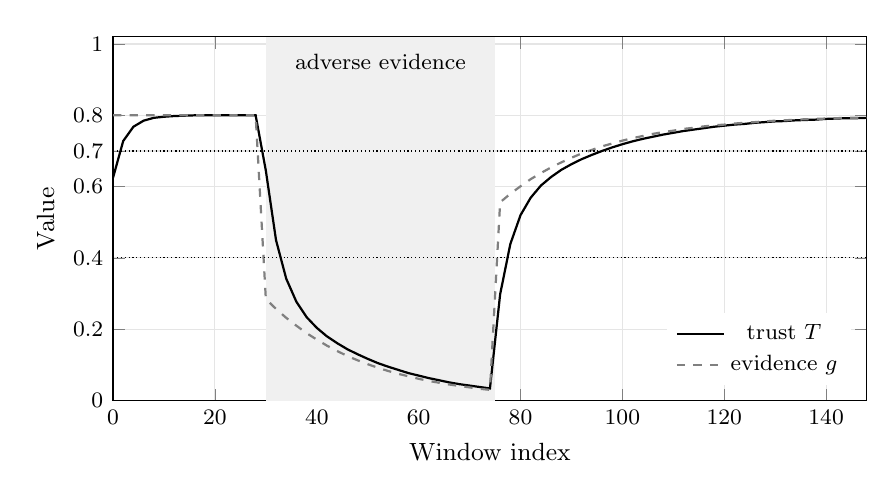
\begin{tikzpicture}
\begin{axis}[
  width=0.92\textwidth, height=6.2cm,
  xlabel={Window index}, ylabel={Value},
  xmin=0, xmax=148, ymin=0, ymax=1.02,
  ytick={0,0.2,0.4,0.6,0.7,0.8,1},
  legend style={at={(0.98,0.04)}, anchor=south east, font=\footnotesize, draw=none, fill=white},
  tick label style={font=\footnotesize}, label style={font=\small},
  grid=major, grid style={gray!20}]
\fill[gray!12] (axis cs:30,0) rectangle (axis cs:75,1.02);
\node[font=\footnotesize, anchor=north] at (axis cs:52.5,1.0) {adverse evidence};
\addplot[thick, black] coordinates {(0,0.625) (2,0.728) (4,0.768) (6,0.785) (8,0.793) (10,0.796) (12,0.798) (14,0.799) (16,0.8) (18,0.8) (20,0.8) (22,0.8) (24,0.8) (26,0.8) (28,0.8) (30,0.645) (32,0.45) (34,0.342) (36,0.277) (38,0.234) (40,0.204) (42,0.18) (44,0.161) (46,0.144) (48,0.13) (50,0.117) (52,0.105) (54,0.095) (56,0.086) (58,0.077) (60,0.07) (62,0.063) (64,0.057) (66,0.051) (68,0.046) (70,0.042) (72,0.038) (74,0.034) (76,0.298) (78,0.439) (80,0.52) (82,0.569) (84,0.603) (86,0.627) (88,0.647) (90,0.663) (92,0.677) (94,0.689) (96,0.7) (98,0.71) (100,0.719) (102,0.727) (104,0.734) (106,0.74) (108,0.746) (110,0.751) (112,0.756) (114,0.76) (116,0.764) (118,0.768) (120,0.771) (122,0.774) (124,0.776) (126,0.779) (128,0.781) (130,0.783) (132,0.784) (134,0.786) (136,0.787) (138,0.788) (140,0.79) (142,0.791) (144,0.792) (146,0.792) (148,0.793)};
\addlegendentry{trust $T$}
\addplot[thick, dashed, gray] coordinates {(0,0.8) (28,0.8) (30,0.285) (32,0.257) (34,0.232) (36,0.21) (38,0.189) (40,0.171) (42,0.154) (44,0.139) (46,0.125) (48,0.113) (50,0.102) (52,0.092) (54,0.083) (56,0.075) (58,0.068) (60,0.061) (62,0.055) (64,0.05) (66,0.045) (68,0.041) (70,0.037) (72,0.033) (74,0.03) (76,0.556) (78,0.58) (80,0.601) (82,0.621) (84,0.638) (86,0.654) (88,0.668) (90,0.681) (92,0.693) (94,0.703) (96,0.713) (98,0.721) (100,0.729) (102,0.736) (104,0.742) (106,0.748) (108,0.753) (110,0.757) (112,0.762) (114,0.765) (116,0.769) (118,0.772) (120,0.774) (122,0.777) (124,0.779) (126,0.781) (128,0.783) (130,0.785) (132,0.786) (134,0.788) (136,0.789) (138,0.79) (140,0.791) (142,0.792) (144,0.793) (146,0.793) (148,0.794)};
\addlegendentry{evidence $g$}
\addplot[thin, densely dotted, black, domain=0:148] {0.7};
\addplot[thin, densely dotted, black, domain=0:148] {0.4};
\end{axis}
\end{tikzpicture}
\caption{Response of the trust update rule to an idealised evidence profile, computed from Equations~\eqref{eq:h}--\eqref{eq:betaupdate}; dotted lines mark the 0.7 and 0.4 band limits}
\label{fig:trustdyn}
\end{figure}

\begin{lstlisting}[float=htbp, language=Python, caption={Beta-reputation state update (\texttt{edge/trust/beta.py})}, label={lst:beta}]
def combine_g(c: float, k: float, h: float) -> float:
    return W_CONSISTENCY * c + W_CORRELATION * k + W_RELIABILITY * h

def update(self, g: float) -> float:
    self.alpha = self.forgetting * self.alpha + g
    self.beta = self.forgetting * self.beta + (1.0 - g)
    return self.alpha / (self.alpha + self.beta)
\end{lstlisting}

\subsection{Physics-Based Attribution}
\label{sec:attribution}

A pump motor is either running or idle, and both its supply current and its vibration reflect that state. Each of the two sensors is therefore an independent witness of the motor state. The operating-state rule classifies each channel from the \emph{median} of its raw window, so that impulsive events such as a tap or a one-sample glitch cannot flip the state:
\begin{equation}
\mathrm{state}(\mathbf{x}) =
\begin{cases}
\textsc{idle}, & \mathrm{median}(\mathbf{x}) \leq b_{\mathrm{idle}}, \\
\textsc{running}, & \mathrm{median}(\mathbf{x}) \geq b_{\mathrm{run}}, \\
\textsc{unclear}, & \text{otherwise.}
\end{cases}
\end{equation}
For current, $b_{\mathrm{idle}} = 0.05$~A and $b_{\mathrm{run}} = 0.3$~A. Vibration depends on how the sensor is mounted, so its bands are learned from the steady windows of the clean baseline: $b_{\mathrm{idle}}$ is 1.5 times the 99.9th percentile of the idle window medians, and $b_{\mathrm{run}}$ lies midway between $b_{\mathrm{idle}}$ and the 5th percentile of the running window medians. On the deployed baseline this gives $b_{\mathrm{idle}} = 0.142$~$g$ and $b_{\mathrm{run}} = 0.314$~$g$. The gap between the bands acts as hysteresis: a window inside it gives no verdict, so motor transitions never produce a violation.

When one channel reports \textsc{idle} and the other \textsc{running}, the machine described by the data is physically impossible and one reading must be false. The suspect is the channel whose state changed most recently while the other stayed constant: a motor that really starts or stops moves both channels together, whereas a single falsified channel moves alone. Algorithm~\ref{alg:attribution} summarises the procedure. An anomaly is attributed as an \emph{attack} on the suspect when physics is violated, and as a \emph{fault} otherwise; when several labels compete, the priority is attack, then fault, then none.

\begin{algorithm}[H]
\caption{Operating-state attribution for one window}
\label{alg:attribution}
\begin{algorithmic}[1]
\Require raw windows $\mathbf{x}_{I}$ (current) and $\mathbf{x}_{V}$ (vibration); channel flags $F$; previous states $s_I^{-}, s_V^{-}$
\Ensure attribution label and suspect channel
\State $s_I \gets \mathrm{state}(\mathbf{x}_I)$, \; $s_V \gets \mathrm{state}(\mathbf{x}_V)$
\If{$\{s_I, s_V\} = \{\textsc{idle}, \textsc{running}\}$}
  \If{$s_I \neq s_I^{-}$ \textbf{and} $s_V = s_V^{-}$} \State suspect $\gets$ current
  \ElsIf{$s_V \neq s_V^{-}$ \textbf{and} $s_I = s_I^{-}$} \State suspect $\gets$ vibration
  \Else \State suspect $\gets$ both
  \EndIf
  \State \Return (\textsc{attack}, suspect, ``physics violation'')
\ElsIf{any channel in $F$ is flagged}
  \State \Return (\textsc{fault}, flagged channels, ``physically consistent anomaly'')
\Else
  \State \Return (\textsc{none}, --, --)
\EndIf
\end{algorithmic}
\end{algorithm}

The rule covers the physically coupled pair of channels on this rig. Temperature, humidity, pressure and gas have no physical partner on the bench and can only be attributed as faults; extending physical coupling to them requires a process with the corresponding relationships, such as discharge pressure in a real pump.

\subsection{Isolation and Self-Healing with an LSTM Digital Twin}

A channel enters isolation when its trust falls below 0.4 and leaves it when trust returns to 0.7; the Suspicious band in between prevents oscillation. While a channel is isolated, its reading is removed from fusion and replaced by a reconstruction from the digital twin, and the dashboard marks the value as \textsc{virtual}.

The twin is a single-layer, unidirectional LSTM~\cite{hochreiter1997lstm}. For each time step $t$ of the 30-sample window, the input $\mathbf{u}_t$ concatenates the six channel values, with the isolated channel set to zero, and a six-element one-hot mask that names the missing channel. The LSTM computes
\begin{align}
\mathbf{i}_t &= \sigma(\mathbf{W}_i \mathbf{u}_t + \mathbf{U}_i \mathbf{h}_{t-1} + \mathbf{b}_i), &
\mathbf{f}_t &= \sigma(\mathbf{W}_f \mathbf{u}_t + \mathbf{U}_f \mathbf{h}_{t-1} + \mathbf{b}_f), \nonumber\\
\mathbf{o}_t &= \sigma(\mathbf{W}_o \mathbf{u}_t + \mathbf{U}_o \mathbf{h}_{t-1} + \mathbf{b}_o), &
\tilde{\mathbf{c}}_t &= \tanh(\mathbf{W}_c \mathbf{u}_t + \mathbf{U}_c \mathbf{h}_{t-1} + \mathbf{b}_c), \nonumber\\
\mathbf{c}_t &= \mathbf{f}_t \odot \mathbf{c}_{t-1} + \mathbf{i}_t \odot \tilde{\mathbf{c}}_t, &
\mathbf{h}_t &= \mathbf{o}_t \odot \tanh(\mathbf{c}_t),
\end{align}
and the reconstruction is $\hat{y} = \mathbf{w}^{\top} \mathbf{h}_{30} + b$. Inputs and target are expressed on a fixed z-score scale computed from the clean training data, so the output is converted back to engineering units exactly.

The deployed twin reconstructs motor current from vibration, the channel that is physically coupled to it; the ambient channels are excluded from its input because they carry no information about current on this rig. It has 32 hidden units and was trained with the Adam optimiser (learning rate 0.01, 30 epochs, mean-squared-error loss) on three bench recordings, with the last 15\% of each recording held out. No training window spans two recordings or a gap in time. Training is performed on the workstation with PyTorch, and the trained weights, scale and residual statistics are saved together as one bundle that the edge loads at start-up, so a model can never be used with a scale it was not trained on.

Substitution is bounded. An uncertainty value $u = \min(t_s/60, 1)$ grows with the elapsed substitution time $t_s$ in seconds; when $u$ exceeds 0.8 (after 48~s) the self-healing layer raises an internal signal that the budget is nearly exhausted, and after 60~s of continuous substitution the self-healing layer escalates to a Safe Pump-Stop. A second escalation path compares the live reading with the twin's reconstruction and escalates when their divergence exceeds a threshold. It is implemented and tested but disabled in the deployed configuration: on clean held-out data, a 3$\sigma$ threshold would have produced false escalations in 4.5\% of windows, which is not acceptable for an action that stops the plant.

\subsection{Safety Supervisor}

The safety supervisor is the only component allowed to switch the pump relay. It acts on four causes: an operator command, a self-healing escalation, a dry-run signature (pump commanded on, past a 5~s spin-up grace, with the current inside the dry-run band for three consecutive frames), and a watchdog that fires when no healthy frame has arrived for 10~s while the pump runs. Every autonomous stop \emph{latches}: the pump stays off until an administrator restarts it through a confirmation dialog. The edge forces the relay off at start-up and at shutdown, and the service manager releases the relay pin after a crash, so every failure mode ends with the pump stopped. Figure~\ref{fig:safetysm} shows the state machine.

\begin{figure}[htbp]
\centering
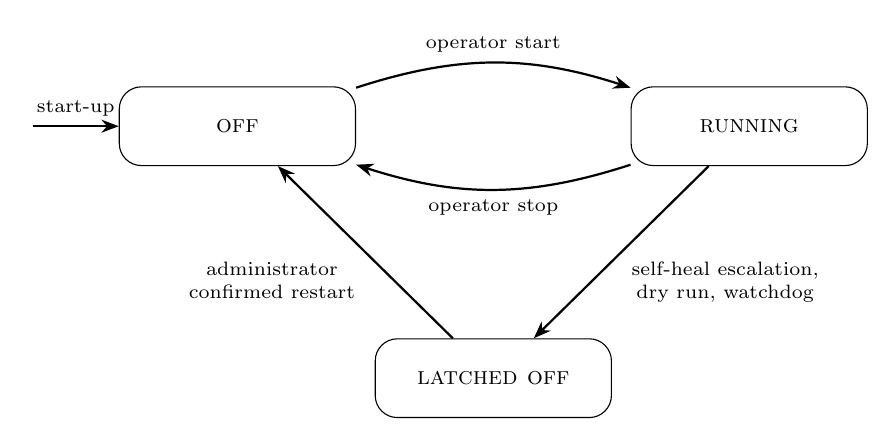
\begin{tikzpicture}[
  st/.style={draw, rounded corners=8pt, minimum width=3.0cm, minimum height=1.0cm, align=center, font=\small, fill=white},
  tr/.style={-{Stealth[length=2.2mm]}, thick},
  tl/.style={font=\scriptsize, align=center}]
  \node[st] (off) at (0,0) {\textsc{off}};
  \node[st] (run) at (6.5,0) {\textsc{running}};
  \node[st] (lat) at (3.25,-3.2) {\textsc{latched off}};
  \draw[tr] (off) to[bend left=18] node[tl, above]{operator start} (run);
  \draw[tr] (run) to[bend left=18] node[tl, below]{operator stop} (off);
  \draw[tr] (run) -- node[tl, below right]{self-heal escalation,\\dry run, watchdog} (lat);
  \draw[tr] (lat) -- node[tl, below left]{administrator\\confirmed restart} (off);
  \draw[tr] (-2.6,0) -- node[tl, above]{start-up} (off);
\end{tikzpicture}
\caption{State machine of the safety supervisor}
\label{fig:safetysm}
\end{figure}

Relay commands travel on their own MQTT topic, separate from scenario injections, so an injected test scenario can never reach the relay. Each transition is reported by the edge as an actuation status (relay state, cause, reason, latched flag and whether a physical relay is attached), and the backend chains every transition into the ledger.

\subsection{Tamper-Evident Audit Ledger}

Safety-relevant events are appended to a hash chain~\cite{haber1991timestamp}. For block $n$ with timestamp $\tau_n$ and payload $P_n$,
\begin{align}
\mathrm{ph}_n &= \mathrm{SHA256}\big(\mathrm{canon}(P_n)\big), \\
H_n &= \mathrm{SHA256}\big(n \,\|\, \tau_n \,\|\, \mathrm{ph}_n \,\|\, H_{n-1}\big), \qquad H_{-1} = 0^{64},
\end{align}
where $\mathrm{canon}$ serialises the payload as JSON with sorted keys and no insignificant whitespace, so that the same payload always produces the same digest, and $\|$ denotes concatenation. Modifying any field of block $n$ changes $\mathrm{ph}_n$ or $H_n$ and breaks the link stored in block $n+1$. Algorithm~\ref{alg:verify} shows the verifier, and Table~\ref{tab:ledgerevents} the events that are chained.

\begin{algorithm}[H]
\caption{Ledger verification}
\label{alg:verify}
\begin{algorithmic}[1]
\Require blocks $B_0, \dots, B_N$ of one device in index order
\Ensure valid, or the index of the first broken block
\State $e \gets 0^{64}$
\For{$n = 0$ \textbf{to} $N$}
  \State \textbf{if} $B_n.\mathrm{ph} \neq \mathrm{SHA256}(\mathrm{canon}(B_n.P))$ \textbf{then return} broken at $n$
  \State \textbf{if} $B_n.\mathrm{prev} \neq e$ \textbf{then return} broken at $n$
  \State \textbf{if} $B_n.H \neq \mathrm{SHA256}(n \,\|\, B_n.\tau \,\|\, B_n.\mathrm{ph} \,\|\, B_n.\mathrm{prev})$ \textbf{then return} broken at $n$
  \State $e \gets B_n.H$
\EndFor
\State \Return valid
\end{algorithmic}
\end{algorithm}

\begin{table}[htbp]
\centering
\caption{Events recorded in the audit ledger}
\label{tab:ledgerevents}
\small
\begin{tabularx}{\textwidth}{@{}l X@{}}
\toprule
\textbf{Event type} & \textbf{Recorded when} \\
\midrule
\texttt{trust\_drop} & A channel's trust crosses below the Malicious limit, with the edge's attribution \\
\texttt{isolate} & A channel is isolated and digital-twin substitution begins \\
\texttt{released\_from\_isolation} & An isolated channel's trust recovers and the real reading is restored \\
\texttt{recover} & A channel returns to the Trusted band \\
\texttt{safe\_stop} & The supervisor stops the pump autonomously \\
\texttt{relay\_command} & An administrator requests a relay change \\
\texttt{relay\_on}, \texttt{relay\_off} & The edge reports a relay transition \\
\texttt{inject} & An administrator starts or cancels a test scenario \\
\texttt{config\_update} & An administrator changes a threshold \\
\bottomrule
\end{tabularx}
\end{table}

\subsection{Scenario Injection}

To evaluate the system with known ground truth, and to let an administrator rehearse incidents live, the edge can transform one channel's readings for a set duration. Eight transforms are implemented (Table~\ref{tab:injections}). In the live path the injection is applied inside the edge, after acquisition and before detection, so it travels the identical path that a real falsified reading would take.

\begin{table}[htbp]
\centering
\caption{Implemented fault and attack injections ($x_t$: true reading, $t$: samples since onset)}
\label{tab:injections}
\small
\begin{tabularx}{\textwidth}{@{}l l X@{}}
\toprule
\textbf{Injection} & \textbf{Class} & \textbf{Injected value} \\
\midrule
Gradual drift & Fault & $x_t + r\,t$ \\
Sudden spike & Fault & $x_t + A$ for the active samples \\
Stuck sensor & Fault & value frozen at onset \\
Bias injection & Attack & $x_t + b$ \\
Ramp injection & Attack & $x_t + r\,t$ \\
Replay & Attack & the channel's own earlier recording \\
Constant spoof & Attack & a constant value $v$ \\
Adaptive stealth & Attack & $x_t + \mathrm{clip}(r\,t, -\delta, \delta)$, kept below a residual bound $\delta$ \\
\bottomrule
\end{tabularx}
\end{table}

\subsection{Backend Services}

The backend subscribes to the edge's telemetry, decision, status and actuation topics. Each message is validated against the contract and written to the database off the hot path. Telemetry frames are additionally fanned out immediately to connected dashboards over a WebSocket, so the live trends move with every sample; decisions, alerts, the live physics state and the relay state are served through REST endpoints that the dashboard polls every one to five seconds (the live state every second and decisions every two). On top of the stored data the backend maintains:

\begin{itemize}
  \item \textbf{Alerts}: one alert per incident, raised at the moments the ledger records them: a trust drop (critical, labelled attack or fault from the edge's attribution), a Safe Pump-Stop (critical) and a dead sensor (warning). Operators acknowledge alerts from the dashboard.
  \item \textbf{Device condition}: a rollup that reports \emph{critical} on a latched Safe Pump-Stop, attacks in a majority (5) of the last 10 decisions, or an isolated channel under a fresh attack; \emph{warning} on an isolated channel or faults and attacks in a majority of the last 10; and \emph{healthy} otherwise.
  \item \textbf{Live state}: the edge's motor-state reading and the twin's reconstructed values, for display.
  \item \textbf{Sensor health}: which channels are currently dead and since when.
\end{itemize}

\paragraph{Security.} Passwords are hashed with bcrypt. Login returns a signed JSON Web Token valid for 15 minutes and a refresh token valid for 7 days that is rotated on use and revoked on logout. Every REST endpoint and the WebSocket validate the token; the WebSocket closes with code 4401 for an invalid token and 4403 for a device the user may not access. Table~\ref{tab:rbac} shows the role permissions and Table~\ref{tab:api} the principal endpoints.

\begin{table}[htbp]
\centering
\caption{Role-based access control}
\label{tab:rbac}
\small
\begin{tabularx}{\textwidth}{@{}X c c c@{}}
\toprule
\textbf{Capability} & \textbf{Operator} & \textbf{Analyst} & \textbf{Administrator} \\
\midrule
View control room, sensors, decisions and history & Yes & Yes & Yes \\
View and acknowledge alerts & Yes & Yes & Yes \\
View, verify and export the audit ledger & -- & Yes & Yes \\
Inject test scenarios & -- & Yes & Yes \\
Start or stop the pump & -- & -- & Yes \\
Thresholds, devices, users and system health & -- & -- & Yes \\
\bottomrule
\end{tabularx}
\end{table}

\begin{table}[htbp]
\centering
\caption{Principal REST and WebSocket endpoints}
\label{tab:api}
\small
\begin{tabularx}{\textwidth}{@{}l l X@{}}
\toprule
\textbf{Method} & \textbf{Path} & \textbf{Purpose} \\
\midrule
POST & \texttt{/api/auth/\{login, refresh, logout\}} & Authentication \\
GET & \texttt{/api/devices/\{id\}/readings} & Telemetry history \\
GET & \texttt{/api/devices/\{id\}/decisions} & Decision history with trust and attribution \\
GET & \texttt{/api/devices/\{id\}/live-state} & Motor state and twin values \\
GET & \texttt{/api/devices/\{id\}/sensor-health} & Dead-sensor status \\
GET, PATCH & \texttt{/api/devices/\{id\}/thresholds} & Detection thresholds (administrator) \\
POST & \texttt{/api/devices/\{id\}/inject} & Start a test scenario (analyst, administrator) \\
GET, POST & \texttt{/api/devices/\{id\}/relay} & Relay state and commands (administrator) \\
GET & \texttt{/api/ledger/\{id\}} & Ledger blocks (analyst, administrator) \\
POST & \texttt{/api/ledger/\{id\}/verify} & Chain verification \\
GET & \texttt{/api/ledger/\{id\}/export} & Ledger export \\
GET, POST & \texttt{/api/alerts}, \texttt{/\{id\}/ack} & Alerts and acknowledgement \\
GET & \texttt{/api/system/health} & Broker, sample rate and latency (administrator) \\
WS & \texttt{/ws?token=\ldots\&device\_id=\ldots} & Live telemetry stream \\
\bottomrule
\end{tabularx}
\end{table}

\subsection{Dashboard}

The dashboard is a React and TypeScript single-page application designed on the principles of ANSI/ISA-101~\cite{isa101}: displays are calm and neutral during normal operation, colour is reserved for abnormal conditions, and every status is conveyed by text as well as by colour. Table~\ref{tab:pages} lists its pages. Two display rules prevent a single noisy window from alarming the operator: the control room shows a fault only when it holds 5 of the last 10 decisions, and a channel that has sent nothing for 10~s is shown as \textsc{no data} rather than with a stale value.

\begin{table}[htbp]
\centering
\caption{Dashboard pages}
\label{tab:pages}
\small
\begin{tabularx}{\textwidth}{@{}l X@{}}
\toprule
\textbf{Page} & \textbf{Content} \\
\midrule
Control room & Live status of all six channels, motor-state physics panel, trust per channel, incident timeline and current verdict \\
Sensor detail & Opened from any channel: live trend, trust history, statistics, health, and the twin's value when substituted \\
Devices & Monitored pumps with their condition and a plain-language explanation of it \\
Device & Device information, scenario injection and the pump relay panel \\
Decisions & Decision log with trust timeline, attribution and reason \\
History & Stored telemetry over a selectable period \\
Alerts & Active and acknowledged alerts with severity and reason \\
Ledger & Hash-chained events and one-click chain verification \\
System & Live architecture view, broker status, sample rate and end-to-end latency \\
Users & Account and role management (administrator) \\
Settings & Connection and display preferences; current detection thresholds \\
\bottomrule
\end{tabularx}
\end{table}

\subsection{Prognosis and Response-Policy Modules}
\label{sec:impl-prognosis-rl}

Two further components of the original design were implemented as modules and verified by unit tests, but are not part of the deployed decision path.

\textbf{Prognosis.} An LSTM prognosis network and its full data pipeline were built against the public PRONOSTIA (FEMTO) bearing run-to-failure dataset~\cite{nectoux2012pronostia}, including the input representation, data-quality rules and remaining-useful-life targets. A remaining-life prediction for the pump needs run-to-failure data from the pump itself, which a bench rig cannot produce; the deployed system therefore reports condition (healthy, warning, critical) from the rollup described above and never presents a remaining-life estimate.

\textbf{Response policy.} The reinforcement-learning layer provides the state vector (machine health, anomaly flag, six trust scores and failure estimate), the action set (continue, reduce weight, isolate sensor, trigger alert, Safe Pump-Stop), a reward that penalises false isolation, missed critical faults and downtime, a simulation environment with synthetic degradation, a deep Q-network training harness and a fallback gate. The deployed system runs the deterministic rule-based policy described in this chapter, which the requirements specify as the fail-safe fallback (FR-RL4). Choosing the reward weights is a policy decision about the acceptable trade-off between false isolation and downtime, and training the learned policy is left as future work.

\section{Functional Description of Modules}

The complete behaviour of the system for one cycle is as follows.

\begin{enumerate}
  \item \textbf{Start-up.} The edge loads the persisted clean baseline, fits the Isolation Forest, the channel flag policy, the consistency provider and the vibration bands on it, loads the twin bundle, forces the relay off and connects to the broker. If no baseline exists, it warms up on live data instead and logs that it has done so.
  \item \textbf{Sampling.} Once per second the sampler reads all drivers, applies any active test injection and publishes the frame.
  \item \textbf{Decision.} The newest 30 frames form a window. The pipeline scores it, updates $c$, $k$, $h$ and the trust of every channel, and runs the attribution rule.
  \item \textbf{Self-healing.} The isolation tracker compares each trust score with the 0.4 and 0.7 limits; isolated channels are substituted by the twin and their substitution clocks are advanced or reset.
  \item \textbf{Safety.} The supervisor checks escalation, dry-run and watchdog conditions and switches the relay if required.
  \item \textbf{Publication.} The decision (flag, severity, attribution, reason, trust, isolation set, substituted values) and any actuation change are published.
  \item \textbf{Backend.} The backend stores the messages, raises alerts and ledger blocks on edge-triggered transitions, updates the device condition and streams the telemetry to the dashboard over the WebSocket.
  \item \textbf{Presentation.} The dashboard redraws the live trends with every frame and refreshes the verdict, trust and physics panels from the REST endpoints within one to two seconds of the decision.
\end{enumerate}

\chapter{System Testing}
\label{ch:testing}

This chapter describes how SHTAPM was tested, from individual functions to the complete system running on the bench rig, and lists representative test cases with their outcomes.

\section{Overview}

\subsection{Testing Strategy}

Testing was carried out at five levels, each answering a different question.

\begin{enumerate}
  \item \textbf{Unit testing.} Does each module behave as specified in isolation? Hardware buses, clocks and the network are replaced by fakes, so driver logic, timing rules and failure handling can be exercised deterministically on any computer.
  \item \textbf{Integration testing.} Do the modules work together? The edge composition is tested as it is wired in the service entry point, and the backend is tested through its real REST and WebSocket routers with an in-memory database. MQTT round-trip tests run against a real Mosquitto broker when one is reachable.
  \item \textbf{Contract testing.} Do the edge, backend and dashboard agree on every message? The shared telemetry, decision, ledger, injection and actuation schemas are validated on both sides by the same tests.
  \item \textbf{Hardware-in-the-loop testing.} Does the system work on the physical rig? A sensor diagnostic script checks every physical sensor, a recording check validates baseline captures, a pre-flight script checks the running system end to end, and fault and attack scenarios are injected live through the dashboard.
  \item \textbf{Evaluation.} How well does it work? Faults and attacks with known ground truth are injected into recorded clean data and replayed through the exact live pipeline. The results are reported in Chapter~\ref{ch:results}.
\end{enumerate}

\subsection{Tools}

Table~\ref{tab:testtools} lists the tools used for automated testing, static checks and hardware validation.

\begin{table}[htbp]
\centering
\caption{Testing and quality tools}
\label{tab:testtools}
\small
\begin{tabularx}{\textwidth}{@{}l X@{}}
\toprule
\textbf{Tool} & \textbf{Use} \\
\midrule
pytest & Unit, integration and contract tests of the edge, backend and simulator \\
Vitest, Testing Library & Component and logic tests of the dashboard in a simulated browser (jsdom) \\
ruff, black & Python linting and formatting \\
ESLint, Prettier, TypeScript compiler & Dashboard linting, formatting and static type checking \\
Sensor diagnostic script & Reads every physical sensor on the Pi and checks range and health \\
Recording check & Validates a baseline capture: frame gaps, motor runs, sensor stability \\
Pre-flight script & End-to-end check of backend, login, broker, database, telemetry rate, latency and ledger \\
\bottomrule
\end{tabularx}
\end{table}

\subsection{Test Environment}

Table~\ref{tab:testenv} lists the environments in which the tests were run. Automated tests run on the workstation without any hardware; hardware-in-the-loop tests run the complete system with the edge on the Raspberry Pi and the motor under the physical sensors.

\begin{table}[htbp]
\centering
\caption{Test environments}
\label{tab:testenv}
\small
\begin{tabularx}{\textwidth}{@{}P{3.4cm} X@{}}
\toprule
\textbf{Environment} & \textbf{Configuration} \\
\midrule
Automated tests & Windows~11 laptop, Python~3.14 with pytest, Node.js~20 with Vitest; sensor buses, clocks and the network replaced by fakes; in-memory SQLite database \\
Hardware-in-the-loop & Raspberry Pi~5 running the edge service and the Mosquitto broker; backend and dashboard on the laptop; laptop and Pi on the same wireless network \\
Evaluation & Recorded bench captures and the SWaT.A1 dataset replayed through the live edge composition on the laptop \\
Test data & Final baseline recording (51.4~min, 2,609 frames, 21 motor runs) and earlier idle, cycling and running recordings of the same rig \\
\bottomrule
\end{tabularx}
\end{table}

\subsection{Test Suite Summary}

Table~\ref{tab:testcounts} shows the automated tests by subsystem. For the Python code the table counts test functions; parametrised functions expand into several cases when the suite runs.

\begin{table}[htbp]
\centering
\caption{Automated tests by subsystem}
\label{tab:testcounts}
\small
\begin{tabularx}{\textwidth}{@{}X r r@{}}
\toprule
\textbf{Subsystem} & \textbf{Test files} & \textbf{Tests} \\
\midrule
Sensor drivers, acquisition and edge runtime & 33 & 357 \\
Preprocessing, detection and injection & 13 & 184 \\
Trust and attribution & 10 & 150 \\
Isolation, self-healing and digital twin & 17 & 169 \\
Safety supervisor and relay & 4 & 47 \\
Prognosis and response-policy modules & 32 & 940 \\
Backend services, API, security and ledger & 41 & 381 \\
Simulator & 4 & 17 \\
Dashboard (frontend) & 36 & 259 \\
\midrule
\textbf{Total} & \textbf{190} & \textbf{2,504} \\
\bottomrule
\end{tabularx}
\end{table}

Table~\ref{tab:testrun} summarises the final run of both suites. No test failed. The eight skipped tests exercise the discovery of a kernel humidity device by directory name, which contains a colon that the Windows file system does not allow; they run on the Raspberry Pi, and every other test, including the MQTT round-trip tests against a live Mosquitto broker, ran on the workstation. The four expected failures are acceptance tests on a synthetic data fixture; each documents a known limitation of that fixture or of an early design choice and is recorded with its root cause in the project's decision log.

\begin{table}[htbp]
\centering
\caption{Final test run}
\label{tab:testrun}
\small
\begin{tabularx}{\textwidth}{@{}X r r r r@{}}
\toprule
\textbf{Suite} & \textbf{Passed} & \textbf{Skipped} & \textbf{Expected failures} & \textbf{Failed} \\
\midrule
Python: edge, backend, simulator (pytest) & 2,358 & 8 & 4 & 0 \\
Dashboard (Vitest) & 259 & 0 & 0 & 0 \\
\bottomrule
\end{tabularx}
\end{table}

\section{Test Cases}

\subsection{Unit and Integration Test Cases}

Table~\ref{tab:unittests} lists representative automated test cases. Each corresponds to a named test in the repository.

{\small
\setlength{\LTpre}{0pt}
\begin{longtable}{@{}P{1.3cm} P{4.6cm} P{6.0cm} P{1.4cm}@{}}
\caption{Representative unit and integration test cases}
\label{tab:unittests}\\
\toprule
\textbf{ID} & \textbf{Test case} & \textbf{Expected result} & \textbf{Result} \\
\midrule
\endfirsthead
\toprule
\textbf{ID} & \textbf{Test case} & \textbf{Expected result} & \textbf{Result} \\
\midrule
\endhead
\bottomrule
\endfoot
\multicolumn{4}{@{}l}{\textit{Acquisition and drivers}} \\
UT-01 & A sensor fails briefly, then recovers & Last good value held; not reported dead & Pass \\
UT-02 & A sensor fails continuously for 5~s & Reported dead after 5~s & Pass \\
UT-03 & ADXL335 converter reads 0 or 1023 counts & Treated as a failed read, not as acceleration & Pass \\
UT-04 & DHT22 fails transiently & Error raised, next read recovers & Pass \\
UT-05 & Broker disconnects while publishing & Frames buffered and replayed in order on reconnect & Pass \\
\multicolumn{4}{@{}l}{\textit{Detection and injection}} \\
UT-06 & Constant spoof injected live on one channel & Only the target channel pinned, for exactly its duration & Pass \\
UT-07 & Replay injection & Copies the channel's own clean values, never earlier injected ones & Pass \\
UT-08 & Adaptive stealth injection & Offset never exceeds its cap & Pass \\
\multicolumn{4}{@{}l}{\textit{Trust and attribution}} \\
UT-09 & Initial Beta prior & Trust exactly 0.5 & Pass \\
UT-10 & Strong spoof evidence & Trust below 0.4 within 3 windows & Pass \\
UT-11 & Healthy evidence & Trust reaches and stays Trusted & Pass \\
UT-12 & Motor really starts (both channels change) & No physics violation & Pass \\
UT-13 & Current alone changes state & Current named as suspect; attack attributed to it only & Pass \\
UT-14 & Tap or one-sample glitch on vibration & Median state unchanged; no violation & Pass \\
UT-15 & Window median inside the hysteresis gap & No verdict & Pass \\
\multicolumn{4}{@{}l}{\textit{Isolation and self-healing}} \\
UT-16 & Trust falls below 0.4 & Channel isolated and substituted & Pass \\
UT-17 & Trust oscillates inside the Suspicious band & Channel stays isolated; no flicker & Pass \\
UT-18 & Trust returns to 0.7 & Channel released, reported once & Pass \\
UT-19 & Substitution reaches 60~s & Escalation and Safe Pump-Stop & Pass \\
UT-20 & A released channel is isolated again & Substitution clock restarts from zero & Pass \\
\multicolumn{4}{@{}l}{\textit{Safety}} \\
UT-21 & Dry-run current after spin-up grace for 3 frames & Latched Safe Pump-Stop & Pass \\
UT-22 & Motor-off current while commanded off & Not a dry run & Pass \\
UT-23 & Watchdog expires & Relay forced off, exactly once & Pass \\
UT-24 & Relay pin that a sensor uses & Configuration refused & Pass \\
\multicolumn{4}{@{}l}{\textit{Backend, security and ledger}} \\
UT-25 & Payload of a stored block modified & Verifier reports the tampered block & Pass \\
UT-26 & Link between two blocks broken & Verifier reports the broken link & Pass \\
UT-27 & Same payload with keys in a different order & Identical payload hash & Pass \\
UT-28 & Login with wrong password or unknown email & Identical generic 401 response & Pass \\
UT-29 & Refresh token reused after rotation & Rejected with 401 & Pass \\
UT-30 & Operator attempts a scenario injection & 403; denial written to the audit log & Pass \\
UT-31 & Non-administrator switches the pump & Rejected & Pass \\
UT-32 & WebSocket without or with an invalid token & Connection refused & Pass \\
UT-33 & Injection command & Published on the advisory topic, never the relay topic & Pass \\
\end{longtable}
}

\subsection{Hardware-in-the-Loop Test Cases}

Table~\ref{tab:hiltests} lists the tests carried out on the physical rig with the complete system running: edge on the Raspberry Pi, backend and dashboard on the workstation. Scenarios were started from the dashboard by an administrator.

{\small
\setlength{\LTpre}{0pt}
\begin{longtable}{@{}P{1.3cm} P{4.6cm} P{4.4cm} P{3.0cm}@{}}
\caption{Hardware-in-the-loop test cases on the bench rig}
\label{tab:hiltests}\\
\toprule
\textbf{ID} & \textbf{Scenario} & \textbf{Expected result} & \textbf{Observed} \\
\midrule
\endfirsthead
\toprule
\textbf{ID} & \textbf{Scenario} & \textbf{Expected result} & \textbf{Observed} \\
\midrule
\endhead
\bottomrule
\endfoot
HT-01 & Sensor diagnostic on the Pi & All physical sensors respond within range & Pass \\
HT-02 & Live dashboard with the motor cycled by hand & Six channels at 1~Hz; no attack verdict & Pass \\
HT-03 & DHT22 dropout when the motor starts & Last value held; not reported dead & Pass \\
HT-04 & Constant spoof, current set to 0~A, motor running, 40~s & \textsc{attack} on current; isolation; \textsc{virtual} value & \textsc{attack} after 23~s; isolated \\
HT-05 & Bias +0.8~A on current, motor off, 40~s & \textsc{attack} on current & \textsc{attack} after 19~s; no false trip \\
HT-06 & Stuck current sensor, motor running, 40~s & \textsc{fault}, not attack & \textsc{fault} \\
HT-07 & Attack held beyond 60~s of substitution & Latched Safe Pump-Stop & Pump trip; latched \\
HT-08 & Second isolation after a release & No premature pump trip & Pass \\
HT-09 & Ledger verification after the session & Chain intact & All 200 blocks intact \\
HT-10 & Loose converter connection (all channels at the rail) & Readings rejected as failed reads & Pass \\
HT-11 & Small in-state bias on running current & Not attributable as attack (physical limit) & As expected; see Section~\ref{sec:limits} \\
\end{longtable}
}

Test HT-11 is recorded deliberately. A falsification that keeps a reading inside its true physical state is consistent with every other sensor on this rig, so no physics-based rule can expose it; Chapter~\ref{ch:results} quantifies this limit.

\chapter{Results and Analysis}
\label{ch:results}

This chapter reports how well SHTAPM performs. It defines the evaluation metrics, describes the data and the injection protocol, presents the results of every stage of the pipeline on real bench data and on the public SWaT dataset, shows the running system, and compares the approach with baselines.

\section{Evaluation Metrics}

\paragraph{Detection.} With $TP$, $FP$, $TN$ and $FN$ counted over windows,
\begin{gather}
\mathrm{Precision} = \frac{TP}{TP + FP}, \qquad
\mathrm{Recall} = \frac{TP}{TP + FN}, \\
F_1 = \frac{2\,\mathrm{Precision}\cdot\mathrm{Recall}}{\mathrm{Precision} + \mathrm{Recall}}, \qquad
\mathrm{FPR} = \frac{FP}{FP + TN}.
\end{gather}
Because window-level scores favour long attacks, \emph{event coverage} (the number of distinct attack events flagged at least once) and \emph{detection delay} (samples from onset to the first flag) are reported as well.

\paragraph{Attribution.} For each injected episode, the attribution of the injected channel is scored in two ways: \emph{settled} (the majority label over the episode's flagged windows) and \emph{episode} (attack if any flagged window was attributed attack). Faults are scored the same way, so a false accusation counts against the method. The \emph{false-attack rate} is the fraction of channel-windows of clean data attributed attack. Since a rule that labels everything ``attack'' would score perfectly on attacks, the summary metric is the balanced accuracy
\begin{equation}
\mathrm{BA} = \tfrac{1}{2}\left(\mathrm{Recall}_{\mathrm{attack}} + \mathrm{Recall}_{\mathrm{fault}}\right).
\end{equation}

\paragraph{Self-healing.} \emph{Time to isolate} (samples from onset to isolation), \emph{virtual coverage} (fraction of the attack during which the twin's value was served), \emph{substitution error} (median absolute error of the served value against the true reading) and \emph{time to release}. The twin's accuracy is also reported as skill against a predictor that always outputs the training mean:
\begin{equation}
\mathrm{skill} = 1 - \frac{\mathrm{RMSE}_{\mathrm{twin}}}{\mathrm{RMSE}_{\mathrm{mean}}}.
\end{equation}

\section{Experimental Setup}

\paragraph{Data.} The main dataset is the final clean baseline recorded on the rig with all physical sensors in place: 51.4~minutes, 2,609 frames, no frame gap longer than 2~s, and 21 motor runs switched by hand at random intervals (motor on 47\% of the time). Earlier recordings of the same rig are used where stated: a 7.2-hour idle recording, a 19-minute on/off cycling recording, a 25-minute motor-running recording and a 70-minute cycling recording. For comparison with published work, detection is also evaluated on the SWaT.A1 dataset~\cite{goh2016swat}, fitting only on its normal-operation file and testing on its attack file (14,997 windows, 35 attack events).

\paragraph{Protocol.} Ground truth on real hardware is obtained by injecting faults and attacks (Table~\ref{tab:injections}) into the recorded clean data at random onsets and replaying the result through the exact live composition of the edge pipeline. Each scenario is injected ten times. Attacks are further divided by measurement into those whose injected reading crosses into the opposite motor state (physically impossible) and those that stay within the true state. Injection magnitudes are fixed evaluation settings, and no threshold was tuned on the evaluation data.

\section{Output/Results}

\subsection{The Clean Baseline Recording}

Figure~\ref{fig:baseline} shows the motor current and vibration measured on the rig during the final baseline recording. The 21 motor runs are clearly visible in both channels: the current rises from zero to about 0.7~A and the vibration from below 0.1~$g$ to about 0.6~$g$ whenever the motor runs. Individual samples show switch-on current surges and occasional vibration spikes from handling the rig; the figure is clipped above 1.2~A and 1.5~$g$ for readability.

\begin{figure}[htbp]
\centering
\begin{tikzpicture}
\begin{groupplot}[
  group style={group size=1 by 2, vertical sep=0.45cm, xlabels at=edge bottom, xticklabels at=edge bottom},
  width=\textwidth, height=4.6cm, xmin=0, xmax=51.5,
  xlabel={Time (min)}, tick label style={font=\footnotesize}, label style={font=\small},
  grid=major, grid style={gray!20}, restrict y to domain=-1:2, clip=true]
\nextgroupplot[ylabel={Current (A)}, ymin=-0.05, ymax=1.2]
\addplot[black, thin] table[x=t, y=current] {data/baseline_series.dat};
\nextgroupplot[ylabel={Vibration ($g$)}, ymin=-0.05, ymax=1.5]
\addplot[black, thin] table[x=t, y=vibration] {data/baseline_series.dat};
\end{groupplot}
\end{tikzpicture}
\caption{Motor current and vibration measured on the rig over the 51.4-minute baseline recording (every third sample shown)}
\label{fig:baseline}
\end{figure}

Figure~\ref{fig:medians} plots the median current against the median vibration of each 30-sample window of the same recording, together with the motor-state bands of the attribution rule. The windows form two well-separated clusters: idle windows near the origin and running windows with both high current and high vibration. Only 3 of 258 windows fall in the transition region of the current band, where the rule gives no verdict. The two off-diagonal regions, high current with no vibration and high vibration with no current, contain no windows at all. These are the physically impossible states that the attribution rule treats as evidence of falsification.

\begin{figure}[htbp]
\centering
\begin{tikzpicture}
\begin{axis}[
  width=0.82\textwidth, height=7.2cm,
  xlabel={Window median current (A)}, ylabel={Window median vibration ($g$)},
  xmin=-0.05, xmax=1.0, ymin=-0.05, ymax=1.1,
  tick label style={font=\footnotesize}, label style={font=\small},
  legend style={at={(0.02,0.98)}, anchor=north west, font=\footnotesize, draw=none, fill=white, fill opacity=0.9, text opacity=1},
  scatter/classes={idle={mark=o, black}, running={mark=triangle, black}, transition={mark=square*, gray}}]
\fill[gray!12] (axis cs:0.3,-0.05) rectangle (axis cs:1.0,0.142);
\fill[gray!12] (axis cs:-0.05,0.314) rectangle (axis cs:0.05,1.1);
\node[font=\scriptsize, align=center] at (axis cs:0.65,0.06) {impossible: current running,\\vibration idle};
\node[font=\scriptsize, align=center, rotate=90] at (axis cs:0.0,0.66) {impossible};
\addplot[scatter, only marks, mark size=1.6pt, scatter src=explicit symbolic] table[x=current, y=vibration, meta=state] {data/window_medians.dat};
\draw[densely dashed] (axis cs:0.05,-0.05) -- (axis cs:0.05,1.1);
\draw[densely dashed] (axis cs:0.3,-0.05) -- (axis cs:0.3,1.1);
\draw[densely dotted] (axis cs:-0.05,0.142) -- (axis cs:1.0,0.142);
\draw[densely dotted] (axis cs:-0.05,0.314) -- (axis cs:1.0,0.314);
\legend{idle windows, running windows, transition windows}
\end{axis}
\end{tikzpicture}
\caption{Window medians of current and vibration from the baseline recording with the motor-state bands (dashed: current bands 0.05~A and 0.3~A; dotted: learned vibration bands 0.142~$g$ and 0.314~$g$; shaded: physically impossible states)}
\label{fig:medians}
\end{figure}

\subsection{False Alarms on Clean Data}

The baseline was fitted on the first 80\% of the recording and scored on the remaining 493 windows, all of them clean, so that every alarm is a false alarm (Table~\ref{tab:holdout}).

\begin{table}[htbp]
\centering
\caption{Hold-out check of the deployed baseline on clean data}
\label{tab:holdout}
\small
\begin{tabularx}{\textwidth}{@{}X l@{}}
\toprule
\textbf{Measure} & \textbf{Result} \\
\midrule
Windows flagged by the Isolation Forest (threshold 0.90) & 98 of 493 (19.9\%) \\
Channel-windows with trust in the Malicious band & 0 on every channel \\
Channels isolated at the end of the hold-out & None \\
Median clean trust per channel & 0.75--0.83 (all $\geq$ 0.7) \\
Learned vibration bands & idle $\leq$ 0.142~$g$, running $\geq$ 0.314~$g$ \\
Steady idle windows classified idle & 152 of 152 (100\%) \\
\bottomrule
\end{tabularx}
\end{table}

The detector flags about one window in five on clean data. This is by design: the detector is a sensitive first stage, and none of these flags reached the Malicious band or caused an isolation, because the trust engine and the physics rule filter them. Every channel's median clean trust lies above 0.7, which guarantees that an isolated channel can always be released once its input is clean again.

\subsection{Detection on Bench Data}

On the final baseline recording, the deployed detector flagged every injected fault (60 of 60) and every injected attack (120 of 120) at a nominal 5\% clean-flag threshold, with a median delay of 6 samples. Window flags alone are not alarms; they become alarms only through trust and attribution.

\subsection{Fault and Attack Attribution}

Table~\ref{tab:attrib} reports attribution on the final baseline for the deployed operating-state rule.

\begin{table}[htbp]
\centering
\caption{Attribution on the final baseline recording (deployed rule, 10 injections per scenario)}
\label{tab:attrib}
\small
\begin{tabularx}{\textwidth}{@{}X l c c@{}}
\toprule
\textbf{Scenario} & \textbf{Truth} & \textbf{Detected} & \textbf{Correctly attributed (settled)} \\
\midrule
Sudden spike (2 samples) & Fault & 8 & 8 \\
Stuck sensor & Fault & 10 & 10 \\
Gradual drift & Fault & 9 & 5 \\
Constant spoof, crossing state & Attack & 10 & 6 \\
Bias injection, crossing state & Attack & 10 & 10 \\
Replay of the other motor state & Attack & 10 & 9 \\
Ramp injection & Attack & 9 & 4 \\
Constant spoof, within state & Attack & 10 & 0 \\
Bias injection, within state & Attack & 9 & 0 \\
Adaptive stealth injection & Attack & 9 & 0 \\
\midrule
Clean data (2,552 channel-windows) & None & -- & \textbf{0 false attacks (0.0\%)} \\
\bottomrule
\end{tabularx}
\end{table}

Grouped by physical measurement, the deployed rule attributed \textbf{73\%} of state-crossing attacks correctly at episode level (32 of 44; 66\% settled) and kept \textbf{85\%} of faults as faults (23 of 27), with \textbf{zero} false attacks on clean data. Attacks that stay within the true motor state were never attributed as attacks (0 of 23): such readings are physically consistent, which is the limit analysed in Section~\ref{sec:limits}. Most remaining fault errors are drifts, which share their waveform with ramp attacks.

Table~\ref{tab:attribstreams} confirms the behaviour on three earlier recordings of the same rig, evaluated with the deployed rule on 26 October 2026.

\begin{table}[htbp]
\centering
\caption{Attribution of the deployed rule on earlier bench recordings}
\label{tab:attribstreams}
\small
\begin{tabularx}{\textwidth}{@{}X c c c@{}}
\toprule
\textbf{Recording} & \textbf{State-crossing attacks} & \textbf{Faults kept as faults} & \textbf{False attacks, clean} \\
\midrule
Idle, 7.2 h & 120/120 (100\%) & 39/79 (49\%)$^{*}$ & 0/4,742 (0.0\%) \\
Cycling, 19 min & 12/12 (100\%) & 5/5 (100\%) & 1/928 (0.1\%) \\
Running, 25 min & 63/70 (90\%) & 36/42 (86\%) & 2/1,594 (0.1\%) \\
\bottomrule
\multicolumn{4}{@{}l}{\footnotesize $^{*}$All idle fault errors are drifts; spikes and stuck sensors were 39/39 correct.}
\end{tabularx}
\end{table}

\subsection{Real Physical Events}

To check that real disturbances are not mistaken for attacks, a guided session on 26 October 2026 produced genuine physical events on the rig (Table~\ref{tab:realevents}). No real event was attributed as an attack, apart from two windows at a motor switch-on, and the only isolation was of a sensor that had genuinely lost power.

\begin{table}[htbp]
\centering
\caption{Attribution of real physical events on the rig}
\label{tab:realevents}
\small
\begin{tabularx}{\textwidth}{@{}P{5.6cm} X P{3.2cm}@{}}
\toprule
\textbf{Real event} & \textbf{Attribution} & \textbf{Isolation} \\
\midrule
Quiet idle & None or fault & None \\
Motor run, untouched & Two attack windows at switch-on, then fault or none & None \\
Tap on the accelerometer, motor off & Fault only & None \\
Tap on the accelerometer, motor running & Fault only & None \\
Accelerometer power removed, motor off & Fault only & None \\
Accelerometer power removed, motor running & Fault only & Vibration (broken sensor) \\
\bottomrule
\end{tabularx}
\end{table}

\subsection{Self-Healing}

Table~\ref{tab:selfheal} reports self-healing for state-crossing attacks on the current channel. The twin used here was not trained on this recording, so the result is out of sample.

\begin{table}[htbp]
\centering
\caption{Self-healing on the final baseline recording (12 attacks per scenario)}
\label{tab:selfheal}
\small
\begin{tabularx}{\textwidth}{@{}X c c@{}}
\toprule
\textbf{Measure} & \textbf{Bias injection} & \textbf{Constant spoof} \\
\midrule
Attacks isolated & 10/12 & 10/12 \\
Time to isolate, median & 17.5 samples ($\approx$ 21~s) & 15 samples ($\approx$ 18~s) \\
Share of attack served by the twin, median & 52\% & 74\% \\
Error without self-healing, median & 0.60~A & 0.57~A \\
Error of the twin's value, median & \textbf{0.079~A} & \textbf{0.12~A} \\
Time to release, median & 38.5 samples & 38.5 samples \\
False isolations on clean data & 0 & 0 \\
\bottomrule
\end{tabularx}
\end{table}

\begin{figure}[htbp]
\centering
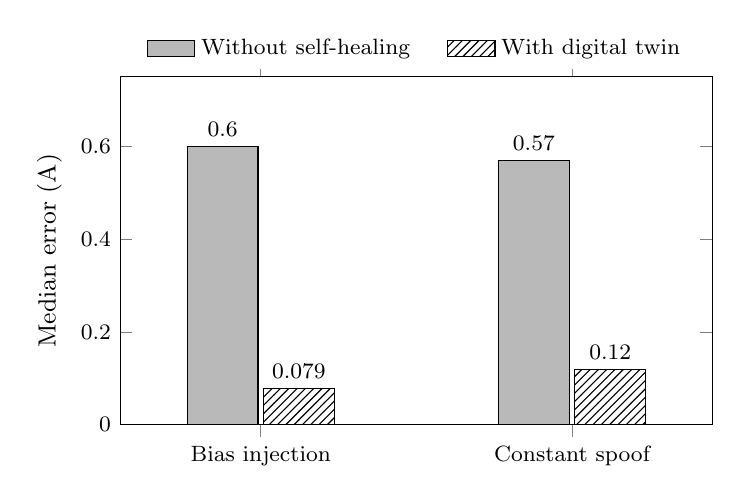
\begin{tikzpicture}
\begin{axis}[
  ybar, area legend, bar width=0.9cm, width=0.75\textwidth, height=6cm,
  ylabel={Median error (A)}, ymin=0, ymax=0.75,
  symbolic x coords={Bias injection, Constant spoof}, xtick=data,
  enlarge x limits=0.45,
  nodes near coords, nodes near coords style={font=\footnotesize, /pgf/number format/fixed, /pgf/number format/precision=3},
  legend style={at={(0.5,1.02)}, anchor=south, legend columns=2, draw=none, font=\footnotesize},
  tick label style={font=\footnotesize}, label style={font=\small}]
\addplot[fill=gray!55, draw=black] coordinates {(Bias injection,0.60) (Constant spoof,0.57)};
\addplot[fill=white, draw=black, postaction={pattern=north east lines}] coordinates {(Bias injection,0.079) (Constant spoof,0.12)};
\legend{Without self-healing, With digital twin}
\end{axis}
\end{tikzpicture}
\caption{Substitution error with and without the digital twin}
\label{fig:healerr}
\end{figure}

The twin removes 79--87\% of the error that the falsified reading would otherwise have introduced. On its own held-out data the deployed twin has a skill of +47.3\% (RMSE 0.188~A against 0.357~A for the mean predictor). Table~\ref{tab:twinloco} shows the leave-one-recording-out evaluation that determined its inputs: a twin that also read the ambient channels failed badly on other days, because ambient conditions carry no information about motor current and shift from day to day.

\begin{table}[htbp]
\centering
\caption{Twin skill, leave-one-recording-out (trained on two recordings, tested on the third)}
\label{tab:twinloco}
\small
\begin{tabularx}{\textwidth}{@{}X c c@{}}
\toprule
\textbf{Test recording} & \textbf{Current and vibration inputs} & \textbf{All five measured inputs} \\
\midrule
Cycling, 70 min & +38.5\% & $-$122.7\% \\
Running, 25 min & +51.3\% & +47.7\% \\
Motor load, five sensors & +64.6\% & $-$61.2\% \\
\bottomrule
\end{tabularx}
\end{table}

\subsection{Live Results on the Running System}

The scenarios of Table~\ref{tab:hiltests} were run on the complete system with the motor under the physical sensors. A constant spoof of the current reading to 0~A while the motor ran was attributed as an attack after 23~s and the channel was isolated and served by the twin; a bias of +0.8~A with the motor off was attributed as an attack after 19~s; a stuck current sensor was reported as a fault; an attack held beyond the 60~s substitution budget produced a latched Safe Pump-Stop; and the ledger verified intact over all 200 blocks of the session. Figures~\ref{fig:ui-login} to \ref{fig:ui-system} show the dashboard.

A later run of the same constant-spoof scenario, captured in the screenshots below, is traced step by step by its audit ledger (Figure~\ref{fig:ui-ledger}). The constant spoof of the current channel was injected at 12:22:56. At 12:23:17, 21~s later, the current channel's trust fell below 0.4 and the channel was isolated, with the digital twin substituting its value (Figure~\ref{fig:ui-attack}: the sensor reported 0.000~A while the twin served 0.791~A, consistent with the running motor). The injection lasted 40~s, but trust recovers only after the window is clean again, so the channel was still isolated when its 60~s substitution budget expired: at 12:24:17, exactly 60~s after isolation, the safety supervisor performed a latched Safe Pump-Stop, and the current channel was released at 12:24:21. Every one of these events was chained, and the verifier confirmed all 200 blocks of the chain intact.

\screenshot{login.png}{0.85}{Login page}{fig:ui-login}
\screenshot{controlroom-normal.png}{1.0}{Control room during normal operation, with the motor idle and both physical witnesses agreeing}{fig:ui-normal}
\screenshot{controlroom-attack.png}{1.0}{Control room during a constant-spoof attack on the current sensor: the physics check reports an impossible state, the channel is attributed as attack and isolated, and the digital twin's value is shown in place of the sensor's 0~A}{fig:ui-attack}
\screenshot{sensor-detail.png}{0.62}{Sensor detail panel for the vibration channel: live trend, statistics and trust history}{fig:ui-detail}
\screenshot{device-injection.png}{0.7}{Device page with the pump relay panel and scenario injection}{fig:ui-inject}
\screenshot{decisions.png}{1.0}{Decisions page: trust of every channel over the last 120 decisions, with the current channel falling to Malicious during the attack, and the decision strip below}{fig:ui-decisions}
\screenshot{decision-detail.png}{1.0}{Decision detail during the attack: attribution, the physical reason and the isolated channel}{fig:ui-decision-detail}
\screenshot{alerts.png}{1.0}{Alerts page with the attack alert and the Safe Pump-Stop that followed}{fig:ui-alerts}
\screenshot{ledger.png}{1.0}{Audit ledger after chain verification, showing the injection, trust drop, isolation, Safe Pump-Stop and release of the attack}{fig:ui-ledger}
\screenshot{system.png}{1.0}{System page: live architecture view and service health}{fig:ui-system}

\subsection{Detection on the SWaT Dataset}

Table~\ref{tab:swat} reports detection on SWaT.A1, with every detector's threshold set to its own nominal 5\% clean-flag rate on the normal-operation data; no attack labels were used to choose thresholds.

\begin{table}[htbp]
\centering
\caption{Detection on SWaT.A1 at a nominal 5\% clean-flag threshold}
\label{tab:swat}
\small
\begin{tabularx}{\textwidth}{@{}X c c c c c@{}}
\toprule
\textbf{Detector} & \textbf{Precision} & \textbf{Recall} & $\mathbf{F_1}$ & \textbf{FPR} & \textbf{Events (of 35)} \\
\midrule
Isolation Forest, deployed preprocessing & 0.418 & 0.332 & 0.370 & 0.065 & 32 \\
Isolation Forest with low-pass filter & 0.548 & 0.562 & 0.555 & 0.065 & 33 \\
Per-channel z-score & 0.799 & 0.687 & 0.739 & 0.024 & 13 \\
Isolation Forest on standardised windows & 0.766 & 0.651 & 0.704 & 0.028 & 23 \\
Maximum of z-score and low-pass Isolation Forest & 0.543 & 0.746 & 0.629 & 0.089 & 33 \\
\bottomrule
\end{tabularx}
\end{table}

\begin{figure}[htbp]
\centering
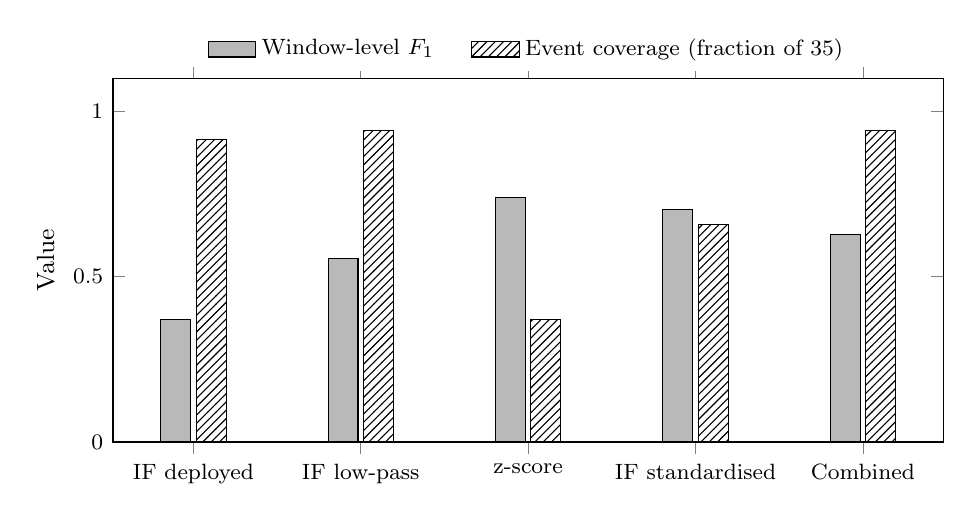
\begin{tikzpicture}
\begin{axis}[
  ybar, area legend, bar width=0.38cm, width=\textwidth, height=6.2cm,
  ymin=0, ymax=1.1, ylabel={Value},
  symbolic x coords={IF deployed, IF low-pass, z-score, IF standardised, Combined},
  xtick=data, x tick label style={font=\footnotesize, align=center},
  enlarge x limits=0.12,
  legend style={at={(0.5,1.02)}, anchor=south, legend columns=2, draw=none, font=\footnotesize},
  tick label style={font=\footnotesize}, label style={font=\small}]
\addplot[fill=gray!55, draw=black] coordinates {(IF deployed,0.370) (IF low-pass,0.555) (z-score,0.739) (IF standardised,0.704) (Combined,0.629)};
\addplot[fill=white, draw=black, postaction={pattern=north east lines}] coordinates {(IF deployed,0.914) (IF low-pass,0.943) (z-score,0.371) (IF standardised,0.657) (Combined,0.943)};
\legend{Window-level $F_1$, Event coverage (fraction of 35)}
\end{axis}
\end{tikzpicture}
\caption{Window-level $F_1$ and event coverage of the detectors on SWaT.A1 (Combined: maximum of z-score and low-pass Isolation Forest)}
\label{fig:swat}
\end{figure}

The two metrics pull apart. The z-score detector has the best window-level $F_1$ but misses 22 of the 35 attacks, while the Isolation Forest flags almost every attack event; it trades precision for coverage. In SHTAPM this trade is deliberate, because the trust engine and the physics rule remove the detector's false alarms downstream (Table~\ref{tab:holdout}). The results also identify a clear improvement: low-pass filtering raises the Isolation Forest's $F_1$ from 0.370 to 0.555 with the same event coverage, and the combined detector raises it by 70\% while flagging 33 of 35 events.

\subsection{System Performance}

The edge sustained its 1~Hz cycle of acquisition, detection, trust, attribution, self-healing and publication for the whole 51.4-minute baseline session with no frame gap longer than 2~s, so one complete decision cycle fits within the one-second sampling period. Measured on the workstation, the path from broker to backend to WebSocket client added a 95th-percentile latency of 3--5~ms, so the sensor-to-screen latency is dominated by the 1~s sampling interval and remains within the 2~s requirement (NFR-P1). The trust update of Section~\ref{sec:trust} isolates a lying sensor within three windows of fully adverse evidence (Figure~\ref{fig:trustdyn}).

\section{Comparative Analysis}

\subsection{Attribution: Operating-State Rule versus Trend-Sign Baseline}

The first attribution rule implemented in the project compared the up/down trend of current and vibration within each window. Table~\ref{tab:attribcompare} compares it with the deployed operating-state rule on the same injected episodes of the final baseline.

\begin{table}[htbp]
\centering
\caption{Attribution methods compared on the final baseline recording}
\label{tab:attribcompare}
\small
\begin{tabularx}{\textwidth}{@{}X c c@{}}
\toprule
\textbf{Measure} & \textbf{Trend-sign rule} & \textbf{Operating-state rule (deployed)} \\
\midrule
State-crossing attacks, episode & 35/42 (83\%) & 32/44 (73\%) \\
State-crossing attacks, settled & 4/42 (10\%) & 29/44 (66\%) \\
Within-state attacks, episode & 12/23 (52\%) & 0/23 (0\%) \\
Faults kept as faults, episode & 10/27 (37\%) & 23/27 (85\%) \\
False attacks on clean data & 23/2,552 (0.9\%) & \textbf{0/2,552 (0.0\%)} \\
Balanced accuracy, episode & 60\% & \textbf{79\%} \\
\bottomrule
\end{tabularx}
\end{table}

\begin{figure}[htbp]
\centering
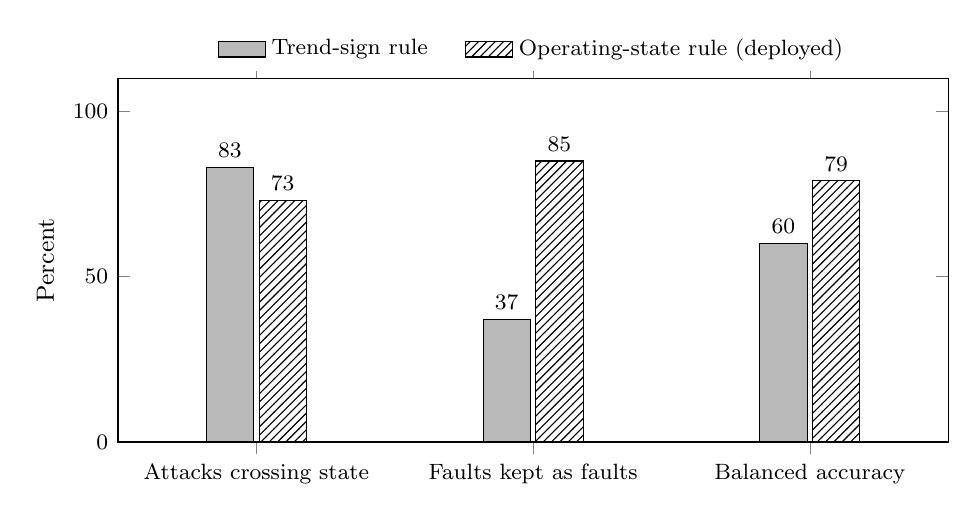
\begin{tikzpicture}
\begin{axis}[
  ybar, area legend, bar width=0.6cm, width=\textwidth, height=6.2cm,
  ymin=0, ymax=110, ylabel={Percent},
  symbolic x coords={Attacks crossing state, Faults kept as faults, Balanced accuracy},
  xtick=data, enlarge x limits=0.25,
  nodes near coords, nodes near coords style={font=\footnotesize, /pgf/number format/fixed, /pgf/number format/precision=3},
  legend style={at={(0.5,1.02)}, anchor=south, legend columns=2, draw=none, font=\footnotesize},
  tick label style={font=\footnotesize}, label style={font=\small}]
\addplot[fill=gray!55, draw=black] coordinates {(Attacks crossing state,83) (Faults kept as faults,37) (Balanced accuracy,60)};
\addplot[fill=white, draw=black, postaction={pattern=north east lines}] coordinates {(Attacks crossing state,73) (Faults kept as faults,85) (Balanced accuracy,79)};
\legend{Trend-sign rule, Operating-state rule (deployed)}
\end{axis}
\end{tikzpicture}
\caption{Episode-level attribution of the two rules}
\label{fig:attribcompare}
\end{figure}

The trend-sign rule's high attack recall is not real discrimination: it also labelled half of the physically consistent attacks and almost two thirds of genuine faults as attacks, and it raised false attacks on clean data. The operating-state rule gives up some recall on attacks to remove false accusations entirely and to keep faults as faults, raising balanced accuracy from 60\% to 79\%. For an operator, an accusation that is never false on clean data is the property that matters.

\subsection{Comparison with Existing Approaches}

Table~\ref{tab:litcompare} in Chapter~\ref{ch:literature} showed that no surveyed class of solution combines predictive maintenance, attack detection, fault--attack disambiguation, dynamic trust, self-healing and decision auditing. SHTAPM implements all six in one pipeline on a low-cost edge device. On detection, its Isolation Forest is used for event coverage rather than window precision, as Table~\ref{tab:swat} shows. On attribution and self-healing, the surveyed works report no directly comparable measurement, so the trend-sign rule and the system without self-healing serve as the baselines above.

\subsection{Achievement of Objectives}

\begin{table}[htbp]
\centering
\caption{Status of the project objectives}
\label{tab:objstatus}
\small
\begin{tabularx}{\textwidth}{@{}l X X@{}}
\toprule
\textbf{ID} & \textbf{Objective} & \textbf{Outcome} \\
\midrule
O1 & Six channels in real time & Achieved: six channels at 1~Hz to the dashboard \\
O2 & Detect anomalies on the edge & Achieved: all injected faults and attacks detected on bench data \\
O3 & Attribute fault or attack & Achieved for physically distinguishable cases: 73\% of state-crossing attacks, 85\% of faults, no false attacks; within-state attacks are a stated physical limit \\
O4 & Dynamic trust per sensor & Achieved: spoofed sensors fall below 0.4; clean trust 0.75--0.83 allows release \\
O5 & Condition monitoring & Achieved: healthy, warning or critical derived continuously \\
O6 & Autonomous self-healing & Achieved: isolation and twin substitution without operator action; error reduced by 79--87\% \\
O7 & Safe stop & Achieved in software: latched Safe Pump-Stop after 60~s, watchdog and dry-run rules verified \\
O8 & Immutable audit trail & Achieved: every safety-relevant decision chained; tampering detected \\
O9 & Professional real-time dashboard & Achieved: role-based access; latency within 2~s \\
O10 & Quantitative evaluation & Achieved: bench recordings and SWaT.A1 \\
\bottomrule
\end{tabularx}
\end{table}

\subsection{Limitations}
\label{sec:limits}

\begin{itemize}
  \item \textbf{Within-state attacks.} A falsification that keeps a reading inside its true physical state is consistent with all other sensors and cannot be attributed by the physics rule. Analytic redundancy through the twin exposes in-state deviations only from about 0.6~A (roughly 80\% of the running current) upward: on clean running data, the twin's residual stayed below 0.48~A in 99.9\% of windows, and a +0.6~A bias exceeded that level in 72\% of windows, against fewer than 2\% for biases up to 0.4~A.
  \item \textbf{Drift and ramp.} A gradual drift fault and a ramp attack are the same waveform and cannot be separated without additional evidence.
  \item \textbf{Coverage of physical coupling.} Only current and vibration have a physical partner on the bench; the other channels can be attributed only as faults.
  \item \textbf{Prototype configuration.} The experiments used the emulated gas source and the in-memory relay (Table~\ref{tab:protoconfig}), and a small DC motor stands in for the pump, so dry-run protection was verified on injected data rather than on a real dry run.
  \item \textbf{Bench security.} The bench broker runs without authentication; production use requires broker authentication and TLS.
\end{itemize}

\chapter{Conclusion \& Future Work}
\label{ch:conclusion}

\section{Conclusion}

This project set out to build a monitoring system for an industrial pump that does not take its sensors at their word. The Self-Healing Trust-Aware Predictive Maintenance System (SHTAPM) achieves this with a complete edge-to-dashboard implementation on low-cost hardware: a Raspberry Pi~5 samples six channels at 1~Hz and runs the whole decision pipeline next to the pump, a FastAPI backend persists, alerts and audits, and a React control-room dashboard presents the result on industrial HMI principles.

The work makes four contributions.

\begin{enumerate}
  \item \textbf{Physics-based fault and attack attribution.} Motor current and vibration are two independent witnesses of whether the motor is running. When they contradict each other, the system attributes an attack to the channel that changed state on its own; otherwise an anomaly is a fault. On real bench recordings with injected falsifications, this rule produced \textbf{no false attack attribution on 2,552 clean channel-windows}, identified the large majority of falsifications that cross a physical state, and kept genuine faults classified as faults. It replaced a trend-based rule that raised false attacks on clean data and called most faults attacks.
  \item \textbf{Evidence-based trust with automatic response.} A Beta-reputation trust score per sensor fuses statistical consistency, physical correlation and historical reliability. Its update rule settles exactly at the level of the evidence, drops a lying sensor to Malicious within three windows and makes it earn its trust back slowly. Trust is coupled directly to isolation and release.
  \item \textbf{Bounded self-healing.} An isolated current sensor is replaced by an LSTM digital-twin reconstruction from vibration. Out of sample, the twin reduced the substitution error from about 0.6~A to about 0.1~A, and the substitution is bounded: after 60~s the supervisor performs a latched Safe Pump-Stop, so the plant is never run on a reconstruction indefinitely.
  \item \textbf{Auditable autonomy.} Every trust drop, isolation, release, pump stop, relay command and test injection is chained into a SHA-256 ledger whose verifier detects any modification of a previous block.
\end{enumerate}

The evaluation also established, and this report states plainly, where the approach stops. A falsification that keeps a reading inside its true physical state is consistent with every other sensor on the rig and cannot be exposed by physics alone; a slow ramp attack is the same waveform as a drift fault; and only the current--vibration pair has a physical partner on the bench. These are limits of the available physical evidence, not of the implementation, and they define the most valuable directions for further work.

Against its objectives (Table~\ref{tab:objstatus}), the project delivers acquisition, detection, attribution, dynamic trust, condition monitoring, self-healing, safe stopping, an immutable audit trail, a secure real-time dashboard and a quantitative evaluation on bench data and the public SWaT dataset. The central idea is validated: physical redundancy between sensors turns ``something is anomalous'' into ``this sensor is lying'', while the plant stays monitored and every autonomous decision remains accountable.

\section{Future Enhancements}

\begin{enumerate}
  \item \textbf{Remaining-useful-life prognosis.} The LSTM prognosis network and its PRONOSTIA data pipeline are implemented. Training and validating it for a pump requires run-to-failure data from pumps of the target type, for example from a utility's maintenance records or an accelerated-wear test rig.
  \item \textbf{Learned response policy.} The reinforcement-learning state, action set, reward structure, simulation environment and deep Q-network harness exist. Once the operators' acceptable trade-off between false isolation and downtime is fixed as reward weights, the policy can be trained in simulation and deployed behind the existing fail-safe gate.
  \item \textbf{Evidence beyond physics for in-state attacks.} Cryptographic attestation or signing of readings at the sensor, physical watermarking of the control signal~\cite{mo2009replay}, and a redundant sensor on the same quantity would expose falsifications that stay within a physical state.
  \item \textbf{Richer physical coupling.} On a real pump, discharge pressure, flow and motor current are physically related. Extending the operating-state rule to these relationships would allow attacks on pressure and other channels to be attributed as well.
  \item \textbf{Detector refinement.} The evaluation shows that low-pass filtering and a combined z-score and Isolation Forest detector improve detection on SWaT; these candidates should be validated on bench data before replacing the deployed detector.
  \item \textbf{Divergence-based escalation.} The twin-divergence escalation path is implemented but disabled. A threshold with an acceptable false-escalation rate should be established on longer clean recordings.
  \item \textbf{Field deployment.} Deploying the relay and the MQ-135 gas sensor on a real pump, measuring the pump's dry-run current, securing the broker with authentication and TLS, and moving the backend to PostgreSQL with TimescaleDB would take the system from the bench to a pilot station.
  \item \textbf{Fleet scale.} The data model already supports many devices. A fleet view, cloud deployment and a distributed ledger would extend the system from one station to a utility's network.
\end{enumerate}


\clearpage
% ----- References -----
\chapter*{REFERENCES}
\addcontentsline{toc}{chapter}{REFERENCES}
% IEEE-style references, numbered in order of first citation. Every entry is a published, verifiable source.
\begingroup
\renewcommand{\chapter}[2]{}% suppress thebibliography's own heading
\begin{thebibliography}{99}
\setlength{\itemsep}{2pt}

\bibitem{lee2014phm} J. Lee, F. Wu, W. Zhao, M. Ghaffari, L. Liao and D. Siegel, ``Prognostics and health management design for rotary machinery systems---Reviews, methodology and applications,'' \emph{Mechanical Systems and Signal Processing}, vol. 42, no. 1--2, pp. 314--334, 2014.

\bibitem{lee2015cps} J. Lee, B. Bagheri and H.-A. Kao, ``A cyber-physical systems architecture for Industry 4.0-based manufacturing systems,'' \emph{Manufacturing Letters}, vol. 3, pp. 18--23, 2015.

\bibitem{susto2015pdm} G. A. Susto, A. Schirru, S. Pampuri, S. McLoone and A. Beghi, ``Machine learning for predictive maintenance: A multiple classifier approach,'' \emph{IEEE Transactions on Industrial Informatics}, vol. 11, no. 3, pp. 812--820, 2015.

\bibitem{ran2019pdmsurvey} Y. Ran, X. Zhou, P. Lin, Y. Wen and R. Deng, ``A survey of predictive maintenance: Systems, purposes and approaches,'' arXiv preprint arXiv:1912.07383, 2019.

\bibitem{zhang2017wdcnn} W. Zhang, G. Peng, C. Li, Y. Chen and Z. Zhang, ``A new deep learning model for fault diagnosis with good anti-noise and domain adaptation ability on raw vibration signals,'' \emph{Sensors}, vol. 17, no. 2, Art. no. 425, 2017.

\bibitem{zhao2019dlhealth} R. Zhao, R. Yan, Z. Chen, K. Mao, P. Wang and R. X. Gao, ``Deep learning and its applications to machine health monitoring,'' \emph{Mechanical Systems and Signal Processing}, vol. 115, pp. 213--237, 2019.

\bibitem{smith2015cwru} W. A. Smith and R. B. Randall, ``Rolling element bearing diagnostics using the Case Western Reserve University data: A benchmark study,'' \emph{Mechanical Systems and Signal Processing}, vol. 64--65, pp. 100--131, 2015.

\bibitem{saxena2008cmapss} A. Saxena, K. Goebel, D. Simon and N. Eklund, ``Damage propagation modeling for aircraft engine run-to-failure simulation,'' in \emph{Proc. International Conference on Prognostics and Health Management (PHM)}, Denver, CO, USA, 2008, pp. 1--9.

\bibitem{nectoux2012pronostia} P. Nectoux, R. Gouriveau, K. Medjaher, E. Ramasso, B. Chebel-Morello, N. Zerhouni and C. Varnier, ``PRONOSTIA: An experimental platform for bearings accelerated degradation tests,'' in \emph{Proc. IEEE International Conference on Prognostics and Health Management (PHM)}, Denver, CO, USA, 2012, pp. 1--8.

\bibitem{purohit2019mimii} H. Purohit, R. Tanabe, K. Ichige, T. Endo, Y. Nikaido, K. Suefusa and Y. Kawaguchi, ``MIMII dataset: Sound dataset for malfunctioning industrial machine investigation and inspection,'' in \emph{Proc. Detection and Classification of Acoustic Scenes and Events Workshop (DCASE)}, 2019, pp. 209--213.

\bibitem{liu2008iforest} F. T. Liu, K. M. Ting and Z.-H. Zhou, ``Isolation forest,'' in \emph{Proc. 8th IEEE International Conference on Data Mining (ICDM)}, 2008, pp. 413--422.

\bibitem{hochreiter1997lstm} S. Hochreiter and J. Schmidhuber, ``Long short-term memory,'' \emph{Neural Computation}, vol. 9, no. 8, pp. 1735--1780, 1997.

\bibitem{malhotra2015lstm} P. Malhotra, L. Vig, G. Shroff and P. Agarwal, ``Long short term memory networks for anomaly detection in time series,'' in \emph{Proc. European Symposium on Artificial Neural Networks (ESANN)}, 2015, pp. 89--94.

\bibitem{wang2023container} R. Wang, H. Qiu, X. Cheng and X. Liu, ``Anomaly detection with a container-based stream processing framework for Industrial Internet of Things,'' \emph{Journal of Industrial Information Integration}, vol. 35, 2023.

\bibitem{goh2017rnn} J. Goh, S. Adepu, M. Tan and Z. S. Lee, ``Anomaly detection in cyber physical systems using recurrent neural networks,'' in \emph{Proc. IEEE 18th International Symposium on High Assurance Systems Engineering (HASE)}, 2017, pp. 140--145.

\bibitem{kravchik2018cnn} M. Kravchik and A. Shabtai, ``Detecting cyber attacks in industrial control systems using convolutional neural networks,'' in \emph{Proc. Workshop on Cyber-Physical Systems Security and Privacy (CPS-SPC)}, ACM, 2018, pp. 72--83.

\bibitem{almiani2020rnn} M. Almiani, A. AbuGhazleh, A. Al-Rahayfeh, S. Atiewi and A. Razaque, ``Deep recurrent neural network for IoT intrusion detection system,'' \emph{Simulation Modelling Practice and Theory}, vol. 101, Art. no. 102031, 2020.

\bibitem{sicari2015road} S. Sicari, A. Rizzardi, L. A. Grieco and A. Coen-Porisini, ``Security, privacy and trust in Internet of Things: The road ahead,'' \emph{Computer Networks}, vol. 76, pp. 146--164, 2015.

\bibitem{roman2013features} R. Roman, J. Zhou and J. Lopez, ``On the features and challenges of security and privacy in distributed Internet of Things,'' \emph{Computer Networks}, vol. 57, no. 10, pp. 2266--2279, 2013.

\bibitem{kolias2017mirai} C. Kolias, G. Kambourakis, A. Stavrou and J. Voas, ``DDoS in the IoT: Mirai and other botnets,'' \emph{Computer}, vol. 50, no. 7, pp. 80--84, 2017.

\bibitem{humayed2017cps} A. Humayed, J. Lin, F. Li and B. Luo, ``Cyber-physical systems security---A survey,'' \emph{IEEE Internet of Things Journal}, vol. 4, no. 6, pp. 1802--1831, 2017.

\bibitem{mitchell2014ids} R. Mitchell and I.-R. Chen, ``A survey of intrusion detection techniques for cyber-physical systems,'' \emph{ACM Computing Surveys}, vol. 46, no. 4, Art. no. 55, 2014.

\bibitem{ding2018survey} D. Ding, Q.-L. Han, Y. Xiang, X. Ge and X.-M. Zhang, ``A survey on security control and attack detection for industrial cyber-physical systems,'' \emph{Neurocomputing}, vol. 275, pp. 1674--1683, 2018.

\bibitem{langner2011stuxnet} R. Langner, ``Stuxnet: Dissecting a cyberwarfare weapon,'' \emph{IEEE Security \& Privacy}, vol. 9, no. 3, pp. 49--51, 2011.

\bibitem{liu2009fdi} Y. Liu, P. Ning and M. K. Reiter, ``False data injection attacks against state estimation in electric power grids,'' in \emph{Proc. 16th ACM Conference on Computer and Communications Security (CCS)}, 2009, pp. 21--32.

\bibitem{mo2009replay} Y. Mo and B. Sinopoli, ``Secure control against replay attacks,'' in \emph{Proc. 47th Annual Allerton Conference on Communication, Control, and Computing}, 2009, pp. 911--918.

\bibitem{cardenas2011attacks} A. A. C\'ardenas, S. Amin, Z.-S. Lin, Y.-L. Huang, C.-Y. Huang and S. Sastry, ``Attacks against process control systems: Risk assessment, detection, and response,'' in \emph{Proc. 6th ACM Symposium on Information, Computer and Communications Security (ASIACCS)}, 2011, pp. 355--366.

\bibitem{urbina2016stealthy} D. I. Urbina, J. A. Giraldo, A. A. C\'ardenas, N. O. Tippenhauer, J. Valente, M. Faisal, J. Ruths, R. Candell and H. Sandberg, ``Limiting the impact of stealthy attacks on industrial control systems,'' in \emph{Proc. ACM SIGSAC Conference on Computer and Communications Security (CCS)}, 2016, pp. 1092--1105.

\bibitem{goh2016swat} J. Goh, S. Adepu, K. N. Junejo and A. Mathur, ``A dataset to support research in the design of secure water treatment systems,'' in \emph{Proc. International Conference on Critical Information Infrastructures Security (CRITIS)}, Springer LNCS 10242, 2017, pp. 88--99.

\bibitem{ahmed2017wadi} C. M. Ahmed, V. R. Palleti and A. P. Mathur, ``WADI: A water distribution testbed for research in the design of secure cyber physical systems,'' in \emph{Proc. 3rd International Workshop on Cyber-Physical Systems for Smart Water Networks (CySWATER)}, ACM, 2017, pp. 25--28.

\bibitem{giraldo2018physics} J. Giraldo, D. Urbina, A. C\'ardenas, J. Valente, M. Faisal, J. Ruths, N. O. Tippenhauer, H. Sandberg and R. Candell, ``A survey of physics-based attack detection in cyber-physical systems,'' \emph{ACM Computing Surveys}, vol. 51, no. 4, pp. 76:1--76:36, 2018.

\bibitem{ahmed2018noise} C. M. Ahmed, J. Zhou and A. P. Mathur, ``Noise matters: Using sensor and process noise fingerprint to detect stealthy cyber attacks and authenticate sensors in CPS,'' in \emph{Proc. 34th Annual Computer Security Applications Conference (ACSAC)}, 2018, pp. 566--581.

\bibitem{chow1984redundancy} E. Y. Chow and A. S. Willsky, ``Analytical redundancy and the design of robust failure detection systems,'' \emph{IEEE Transactions on Automatic Control}, vol. 29, no. 7, pp. 603--614, 1984.

\bibitem{isermann2005fdd} R. Isermann, ``Model-based fault-detection and diagnosis---Status and applications,'' \emph{Annual Reviews in Control}, vol. 29, no. 1, pp. 71--85, 2005.

\bibitem{pasqualetti2013identification} F. Pasqualetti, F. D\"orfler and F. Bullo, ``Attack detection and identification in cyber-physical systems,'' \emph{IEEE Transactions on Automatic Control}, vol. 58, no. 11, pp. 2715--2729, 2013.

\bibitem{teixeira2015secure} A. Teixeira, I. Shames, H. Sandberg and K. H. Johansson, ``A secure control framework for resource-limited adversaries,'' \emph{Automatica}, vol. 51, pp. 135--148, 2015.

\bibitem{josang2002beta} A. J{\o}sang and R. Ismail, ``The beta reputation system,'' in \emph{Proc. 15th Bled Electronic Commerce Conference}, 2002, pp. 2502--2511.

\bibitem{ganeriwal2008reputation} S. Ganeriwal, L. K. Balzano and M. B. Srivastava, ``Reputation-based framework for high integrity sensor networks,'' \emph{ACM Transactions on Sensor Networks}, vol. 4, no. 3, pp. 15:1--15:37, 2008.

\bibitem{bao2012dynamic} F. Bao and I.-R. Chen, ``Dynamic trust management for Internet of Things applications,'' in \emph{Proc. International Workshop on Self-Aware Internet of Things (Self-IoT)}, San Jose, CA, USA, 2012, pp. 1--6.

\bibitem{bao2012trust} F. Bao and I.-R. Chen, ``Trust management for the Internet of Things and its application to service composition,'' in \emph{Proc. IEEE International Symposium on a World of Wireless, Mobile and Multimedia Networks (WoWMoM)}, 2012, pp. 1--6.

\bibitem{yan2014trust} Z. Yan, P. Zhang and A. V. Vasilakos, ``A survey on trust management for Internet of Things,'' \emph{Journal of Network and Computer Applications}, vol. 42, pp. 120--134, 2014.

\bibitem{motmi2022elithe} A. Motmi, S. Alhazmi, A. Abu-Khadrah, M. Al-Akhras and F. Alhosban, ``Trust management in Industrial Internet of Things using a trusted E-Lithe protocol,'' \emph{International Journal of Advanced Computer Science and Applications}, vol. 13, no. 2, 2022.

\bibitem{mnih2015dqn} V. Mnih, K. Kavukcuoglu, D. Silver, A. A. Rusu, J. Veness, M. G. Bellemare \emph{et al.}, ``Human-level control through deep reinforcement learning,'' \emph{Nature}, vol. 518, no. 7540, pp. 529--533, 2015.

\bibitem{nguyen2023drl} T. T. Nguyen and V. J. Reddi, ``Deep reinforcement learning for cyber security,'' \emph{IEEE Transactions on Neural Networks and Learning Systems}, vol. 34, no. 8, pp. 3779--3795, 2023.

\bibitem{tao2019twin} F. Tao, H. Zhang, A. Liu and A. Y. C. Nee, ``Digital twin in industry: State-of-the-art,'' \emph{IEEE Transactions on Industrial Informatics}, vol. 15, no. 4, pp. 2405--2415, 2019.

\bibitem{haber1991timestamp} S. Haber and W. S. Stornetta, ``How to time-stamp a digital document,'' \emph{Journal of Cryptology}, vol. 3, no. 2, pp. 99--111, 1991.

\bibitem{nakamoto2008bitcoin} S. Nakamoto, ``Bitcoin: A peer-to-peer electronic cash system,'' 2008. [Online]. Available: https://bitcoin.org/bitcoin.pdf

\bibitem{dorri2017optimized} A. Dorri, S. S. Kanhere and R. Jurdak, ``Towards an optimized blockchain for IoT,'' in \emph{Proc. IEEE/ACM Second International Conference on Internet-of-Things Design and Implementation (IoTDI)}, 2017, pp. 173--178.

\bibitem{isa101} International Society of Automation, \emph{ANSI/ISA-101.01-2015: Human Machine Interfaces for Process Automation Systems}, Research Triangle Park, NC, USA, 2015.

\end{thebibliography}
\endgroup

\clearpage

% ----- Appendices -----
\appendix
\renewcommand{\thechapter}{\Alph{chapter}}
\renewcommand{\thesection}{\Roman{section}}
\section{Appendix A: Details of list of publications related to this project}

\begin{table}[H]
\centering
\renewcommand{\arraystretch}{1.4}
\begin{tabularx}{\textwidth}{@{}p{5.2cm} X@{}}
\toprule
\textbf{Author Names} & Prof.\ Tejashwini A G, Durgashree R, Keerthi S, Yeshwanth L B \\
\textbf{Paper Title} & Self-Healing Trust-Aware Predictive Maintenance: Physics-Based Fault and Attack Attribution for Industrial Pump Monitoring at the Edge \\
\textbf{Name of the Conference or Journal} & Manuscript in preparation \\
\textbf{Place of the Conference} & -- \\
\textbf{Date of Conference} & -- \\
\bottomrule
\end{tabularx}
\end{table}

\clearpage

\section{Appendix B: Similarity report, AI Generated report}

The similarity report and the AI-generated-content report produced by the institution's plagiarism-detection software for this report are attached on the following pages.

\clearpage

\section{Appendix C: Sustainable Development Goals (SDGs) Addressed}

\begin{center}
\fbox{\begin{minipage}{0.9\textwidth}
\centering
\vspace{6pt}
{\large\textbf{SDG 9: Industry, Innovation and Infrastructure}}\\[4pt]
Build resilient infrastructure, promote inclusive and sustainable industrialisation and foster innovation.
\vspace{6pt}
\end{minipage}}
\end{center}

\paragraph{Justification.} SHTAPM contributes most directly to SDG~9, and in particular to the following targets.

\begin{itemize}
  \item \textbf{Target 9.1, resilient infrastructure.} Pumping stations are critical infrastructure for water supply and sanitation. SHTAPM makes such a station resilient to both of the threats that compromise its monitoring: failing sensors and falsified sensors. It detects them, isolates the affected input, keeps the station monitored through a digital-twin reconstruction and stops the pump safely when trust cannot be restored, so that a single compromised sensor no longer blinds the operator or damages the machine.
  \item \textbf{Target 9.4, upgrading industry with clean and efficient technology.} Condition monitoring replaces fixed-interval servicing with maintenance driven by the measured state of the machine, reducing unnecessary interventions, unplanned downtime and the waste associated with premature part replacement.
  \item \textbf{Target 9.5, enhancing research and technological capability.} The project shows that intelligent, trustworthy monitoring can run on a low-cost edge computer with commodity sensors and open-source software. This lowers the barrier for small utilities and industries in developing regions to adopt secure predictive-maintenance technology, and its physics-based attribution method is a research contribution in its own right.
\end{itemize}

In addition, the tamper-evident audit ledger provides the accountability that autonomous decisions in infrastructure require, supporting trustworthy adoption of automation in essential services.


\end{document}
